% sgt: version control at the level of what you asked for
% Build with ./build.sh
\PassOptionsToPackage{expansion=true,protrusion=true}{microtype}
\documentclass[sigconf,review,anonymous]{acmart}

\AtBeginDocument{%
  \providecommand\BibTeX{{\normalfont B\kern-0.5em{\scshape i\kern-0.25em b}\kern-0.8em\TeX}}}
\setcopyright{none}
\copyrightyear{2027}
\acmYear{2027}
\acmConference[CHI '27]{CHI Conference on Human Factors in Computing Systems}{April 2027}{Yokohama, Japan}
\acmBooktitle{CHI '27}
\settopmatter{printacmref=false}
\renewcommand\footnotetextcopyrightpermission[1]{}

% ---------------------------------------------------------------------------
% Shared visual language for every figure in this paper.
% One palette, one glyph set, one rail geometry. Figures reuse these so a
% reader who learns the notation once in Figure 1 can read all of them.
% ---------------------------------------------------------------------------
\usepackage{tikz}
\usetikzlibrary{calc,positioning,arrows.meta,decorations.pathreplacing,
                decorations.pathmorphing,fit,backgrounds,shapes.geometric,
                patterns,patterns.meta}
\usepackage{xcolor}
\usepackage{booktabs}
% newtxmath (loaded by acmart when the ACM fonts are present) already supplies
% the AMS symbols we use, and loading amssymb on top of it redefines \Bbbk.
\providecommand{\checkmark}{\ensuremath{\surd}}

% Long command strings and qualified symbol names are unbreakable words in a
% narrow column, so let TeX stretch a line rather than run it into the gutter.
\setlength{\emergencystretch}{0.8em}

% Every command line in this paper is typed literally, so the typewriter font
% must not turn -- into a dash or `' into curly quotes.
\DisableLigatures{encoding=*, family=tt*}
\usepackage{upquote}

% --- palette ---------------------------------------------------------------
\definecolor{sgtInk}{HTML}{1B1F24}
\definecolor{sgtGrey}{HTML}{8A8F96}
\definecolor{sgtWash}{HTML}{EFECE6}
\definecolor{sgtPaper}{HTML}{FBFAF8}
\definecolor{fRate}{HTML}{C0701A}   % rate limiting
\definecolor{fCache}{HTML}{14736C}  % caching
\definecolor{fRetry}{HTML}{6A4A9E}  % retry policy
\definecolor{fExport}{HTML}{A83252} % export
\definecolor{fIdx}{HTML}{3A6EA5}    % database index (colleague's work)
% Each request colour has a wash used for fills behind text, so a coloured
% region and a coloured mark can sit next to each other without competing.
\definecolor{wRate}{HTML}{FAEEE1}
\definecolor{wCache}{HTML}{E3F0EE}
\definecolor{wRetry}{HTML}{ECE7F5}
\definecolor{wExport}{HTML}{F8E7EB}
\definecolor{wIdx}{HTML}{E6EDF5}
\definecolor{wGrey}{HTML}{EEEFF0}

% --- type ------------------------------------------------------------------
\newcommand{\cmd}[1]{\texttt{\small #1}}
\newcommand{\placeholder}[1]{{\color{red}\sffamily\small [#1]}}
% the typewriter fonts have no em dash, so quoted terminal output borrows one
\newcommand{\ttdash}{\textrm{\,\textemdash\,}}
% A qualified name like api.py::handle is one unbreakable word wide enough to
% overrun a column, so allow a line to end after the file and resume at the
% function. Nothing else in the name may break.
\ExplSyntaxOn
\NewDocumentCommand \sym { m }
  { \group_begin:
    \tl_set:Nn \l_tmpa_tl {#1}
    \tl_replace_all:Nnn \l_tmpa_tl { :: } { ::\allowbreak }
    \texttt { \small \l_tmpa_tl }
    \group_end: }
\ExplSyntaxOff
\newcommand{\flab}[1]{{\sffamily\bfseries\scriptsize #1}}
\newcommand{\ftiny}[1]{{\sffamily\scriptsize #1}}
\newcommand{\fmini}[1]{{\sffamily\fontsize{5.4}{6}\selectfont #1}}
% a symbol name inside a figure, sized to sit beside 5 to 6pt sans labels
\newcommand{\fsym}[1]{{\ttfamily\fontsize{5.2}{6}\selectfont #1}}

% --- quoted terminal output ------------------------------------------------
% Every block in the walkthrough is what the command printed. The typewriter
% font has none of the marks sgt uses, so each one is drawn or borrowed from the
% roman font and the rest of the line stays in the terminal's font.
% sgt quotes shell words with a backtick and an apostrophe, and both have to
% print as the terminal prints them rather than as a matched curly pair.
\begingroup
\catcode`\'=\active \catcode`\`=\active
\gdef\sgtupquotes{\catcode39=\active \catcode96=\active
  \def'{\textquotesingle}\def`{\textasciigrave}}
\endgroup
\newenvironment{out}
  {\par\addvspace{1.0ex}\begingroup
   \ttfamily\fontsize{6.9}{8.5}\selectfont\raggedright
   \setlength{\parindent}{0pt}%
   \sgtupquotes
   \begin{list}{}{\setlength{\leftmargin}{2.0mm}\setlength{\rightmargin}{0pt}%
                  \setlength{\itemindent}{0pt}\setlength{\labelsep}{0pt}%
                  \setlength{\labelwidth}{0pt}\setlength{\topsep}{0pt}%
                  \setlength{\partopsep}{0pt}\setlength{\parsep}{0pt}%
                  \setlength{\itemsep}{0pt}}%
   \item[]}
  {\end{list}\endgroup\addvspace{1.0ex}}
\newcommand{\ttdot}{\textrm{\,\textperiodcentered\,}}
\newcommand{\ttdisc}{\textrm{\textbullet}}
\newcommand{\ttok}{\textrm{$\checkmark$}}
\newcommand{\ttundo}{\textrm{$\curvearrowleft$}}
\newcommand{\ttnew}{\textrm{$\circ$}}
\newcommand{\ttfull}{\textcolor{sgtInk}{\rule[-0.04ex]{0.62ex}{1.0ex}}\hspace{0.32ex}}
% A column of the history in which a checkpoint has no edits at all. sgt prints a
% middle dot there rather than a space, so a bar is as wide as the history and not
% as wide as the checkpoint, and two checkpoints' bars can be read against each
% other. Set in a box of the block's own width so that they line up.
% Raised to the blocks' own centre: they run from -0.04ex to 0.96ex, and a period
% centred on the x-height sits visibly below that.
\newcommand{\ttempty}{\makebox[0.62ex][c]{%
  \raisebox{0.2ex}{\textcolor{sgtGrey!70}{\textrm{\textperiodcentered}}}}\hspace{0.32ex}}
\newcommand{\ttwarn}{\tikz[baseline=-0.3mm]{%
  \draw[line width=0.35pt, color=sgtInk] (0,0)--(1.35mm,0)--(0.675mm,1.25mm)--cycle;}}
\newcommand{\ttfork}{\textrm{$\pitchfork$}}
\newcommand{\ttleft}{\textrm{$\blacktriangleleft$}}
\newcommand{\ttright}{\textrm{$\blacktriangleright$}}
\newcommand{\ttarrow}{\textrm{$\rightarrow$}}
\newcommand{\ttrule}{\textcolor{sgtGrey}{\rule[0.45ex]{1.6ex}{0.35pt}}}
% the terminal draws its tree with box-drawing characters no font in this
% document has, so each one is a pair of rules at the same weight
\newcommand{\ttvert}{\tikz[baseline=0pt]{%
  \draw[line width=0.3pt, color=sgtGrey] (0,-1.2mm) -- (0,2.1mm);}}
\newcommand{\ttbranch}{\tikz[baseline=0pt]{%
  \draw[line width=0.3pt, color=sgtGrey] (0,-1.2mm) -- (0,2.1mm);
  \draw[line width=0.3pt, color=sgtGrey] (0,0.55mm) -- (1.7mm,0.55mm);}\hspace{0.25mm}}
\newcommand{\ttlast}{\tikz[baseline=0pt]{%
  \draw[line width=0.3pt, color=sgtGrey] (0,2.1mm) -- (0,0.55mm) -- (1.7mm,0.55mm);}%
  \hspace{0.25mm}}

% --- geometry --------------------------------------------------------------
% One op glyph is 2\opsz across, and the thumbnails at the end of this file
% redeclare all three of these at about three fifths the size, because a
% thumbnail packs its marks closer together than a full page figure does and at
% full size the neighbours touch and read as one bar rather than three edits.
\newlength{\opsz}\setlength{\opsz}{1.15mm}
\newlength{\oprad}\setlength{\oprad}{1.32mm}
\newcommand{\ckpth}{1.55}

\tikzset{
  rail/.style        = {line width=1.5pt, color=#1!22, line cap=round},
  rail/.default      = sgtGrey,
  raildim/.style     = {line width=1.5pt, color=sgtGrey!18, line cap=round},
  commitcol/.style   = {line width=0.35pt, color=sgtGrey!55, densely dotted},
  nowrule/.style     = {line width=0.6pt, color=sgtInk!70},
  dep/.style         = {line width=0.35pt, color=sgtGrey!70,
                        -{Straight Barb[length=1.1mm,width=1.1mm]}},
  % An arrowhead in these figures means a direction, so a relation that holds
  % equally both ways is drawn without one. Figure 2 pairs this with the same arc
  % dotted, and the reader then has one shape whose solid form is a relation the
  % system recorded and whose dotted form is one it did not.
  share/.style       = {line width=0.35pt, color=sgtGrey!70},
  card/.style        = {rounded corners=0.6mm, line width=0.4pt},
  note/.style        = {font=\sffamily\fontsize{5.6}{6.4}\selectfont, color=sgtInk!75,
                        inner sep=0.3mm},
  lbl/.style         = {font=\sffamily\fontsize{6.2}{7}\selectfont, color=sgtInk!85,
                        inner sep=0.3mm},
  hd/.style          = {font=\sffamily\bfseries\fontsize{6.6}{7.4}\selectfont,
                        color=sgtInk, inner sep=0.3mm},
}

% --- op glyphs -------------------------------------------------------------
% Five kinds, told apart by shape so they survive greyscale printing.
% add: filled square.  extend: filled square with an open left edge.
% rework: filled disc.  prune: hollow square with a slash.  move: right triangle.
\newcommand{\opadd}[3]{\fill[#3] ($(#1,#2)+(-\opsz,-\opsz)$) rectangle ($(#1,#2)+(\opsz,\opsz)$);}
\newcommand{\opext}[3]{%
  \fill[#3] ($(#1,#2)+(-\opsz,-\opsz)$) rectangle ($(#1,#2)+(\opsz,\opsz)$);
  \fill[sgtPaper] ($(#1,#2)+(-\opsz,-0.42mm)$) rectangle ($(#1,#2)+(-0.28mm,0.42mm)$);}
\newcommand{\oprew}[3]{\fill[#3] (#1,#2) circle (\oprad);}
\newcommand{\opprune}[3]{%
  \draw[#3, line width=0.45pt, fill=sgtPaper]
    ($(#1,#2)+(-\opsz,-\opsz)$) rectangle ($(#1,#2)+(\opsz,\opsz)$);
  \draw[#3, line width=0.45pt] ($(#1,#2)+(-0.8mm,-0.8mm)$) -- ($(#1,#2)+(0.8mm,0.8mm)$);}
\newcommand{\opmove}[3]{%
  \fill[#3] ($(#1,#2)+(-\opsz,-1.25mm)$) -- ($(#1,#2)+(-\opsz,1.25mm)$)
            -- ($(#1,#2)+(1.45mm,0)$) -- cycle;}
\newcommand{\opghost}[3]{%
  \draw[#3, draw opacity=0.55, line width=0.45pt, densely dotted, fill=sgtPaper]
    ($(#1,#2)+(-\opsz,-\opsz)$) rectangle ($(#1,#2)+(\opsz,\opsz)$);}
% a checkpoint: a tick that crosses the rail
\newcommand{\ckpt}[3]{\draw[#3, line width=0.55pt] (#1,{#2-\ckpth}) -- (#1,{#2+\ckpth});}

% --- diff hunk stripe, for drawing a git commit as the thing it is ---------
% \hunk{x}{y}{width}{color}
\newcommand{\hunk}[4]{\fill[#4!85, rounded corners=0.25mm] (#1,#2) rectangle ($(#1,#2)+(#3,0.85mm)$);}

% ---------------------------------------------------------------------------
% Shared figure devices. Four of them, reused in every figure, so a reader who
% works out what a tab or a hand means in Figure 1 never has to work it out
% again. All of them assume a picture with x=1mm, y=1mm.
% ---------------------------------------------------------------------------

% (1) A panel: a rounded card lifted off the page by a soft offset shadow, with
% a coloured tab straddling its top-left corner that names it.
% \panel{x}{y}{width}{height}{colour}{TAB TEXT}
\newcommand{\panel}[6]{%
  \fill[sgtInk!8, rounded corners=1.2mm]
    ({#1+0.55},{#2-0.55}) rectangle ({#1+#3+0.55},{#2+#4-0.55});
  \fill[sgtPaper, rounded corners=1.2mm] (#1,#2) rectangle ({#1+#3},{#2+#4});
  \draw[rounded corners=1.2mm, line width=0.3pt, color=sgtInk!15]
    (#1,#2) rectangle ({#1+#3},{#2+#4});
  \node[anchor=south west, inner xsep=1.15mm, inner ysep=0.6mm, fill=#5,
        rounded corners=0.55mm, text=white,
        font=\sffamily\bfseries\fontsize{5.3}{6}\selectfont]
    at ({#1+1.3},{#2+#4-1.25}) {#6};}

% A panel with no tab, for a region that needs the card shape without a name.
\newcommand{\plainpanel}[5]{%
  \fill[sgtInk!8, rounded corners=1.2mm]
    ({#1+0.55},{#2-0.55}) rectangle ({#1+#3+0.55},{#2+#4-0.55});
  \fill[#5, rounded corners=1.2mm] (#1,#2) rectangle ({#1+#3},{#2+#4});
  \draw[rounded corners=1.2mm, line width=0.3pt, color=sgtInk!15]
    (#1,#2) rectangle ({#1+#3},{#2+#4});}

% (2) Who wrote it. The developer writes the request and the agent writes the
% code, and that split is the paper's subject, so it gets a mark of its own.
% \whodev{x}{y}{colour}   \whoagent{x}{y}{colour}
\newcommand{\whodev}[3]{%
  \fill[#3] (#1,{#2+0.52}) circle (0.5);
  \begin{scope}
    \clip ({#1-1.05},{#2-1.1}) rectangle ({#1+1.05},{#2-0.16});
    \fill[#3] (#1,{#2-0.2}) circle (0.9);
  \end{scope}}
\newcommand{\whoagent}[3]{%
  \draw[color=#3, line width=0.26pt] (#1,{#2+1.28}) -- (#1,{#2+0.92});
  \fill[#3] (#1,{#2+1.38}) circle (0.14);
  \fill[#3, rounded corners=0.24mm]
    ({#1-0.82},{#2-0.72}) rectangle ({#1+0.82},{#2+0.92});
  \fill[sgtPaper] ({#1-0.4},{#2+0.24}) circle (0.155);
  \fill[sgtPaper] ({#1+0.4},{#2+0.24}) circle (0.155);
  \fill[sgtPaper] ({#1-0.38},{#2-0.32}) rectangle ({#1+0.38},{#2-0.2});}

% (3) An annotation: a thin curved leader from the thing to a short label.
% \annot{from x}{from y}{to x}{to y}{bend}{colour}
\newcommand{\annot}[6]{%
  \draw[color=#6!70, line width=0.32pt, bend left=#5,
        -{Straight Barb[length=0.85mm,width=0.9mm]}] (#1,#2) to (#3,#4);}
\tikzset{
  acc/.style     = {font=\sffamily\bfseries\fontsize{5.4}{6.2}\selectfont,
                    color=#1, inner sep=0.3mm},
  acc/.default   = sgtInk,
  tag/.style     = {font=\sffamily\fontsize{5.2}{6}\selectfont, inner xsep=0.7mm,
                    inner ysep=0.35mm, rounded corners=0.4mm},
}

% (4) A highlighted span inside a line of code, the way an editor shows one.
% \hispan{x}{y}{width}{wash colour}
\newcommand{\hispan}[4]{%
  \fill[#4, rounded corners=0.3mm] (#1,{#2-0.75}) rectangle ({#1+#3},{#2+1.25});}

% ---------------------------------------------------------------------------
% Operation thumbnails. Each is 12mm wide and sits on the text baseline, so
% the same picture can head a paragraph in the walkthrough and appear in the
% grid in Section 5. Every thumbnail shows the state before the command on the
% left and the state after it on the right.
% ---------------------------------------------------------------------------
% A thumbnail is 12.6mm wide and has to hold three marks on each side of an
% arrow, so the marks are drawn at three fifths the size they take on a full
% page. What survives the reduction is the silhouette, which is what tells one
% kind of edit from another, and what the reduction buys is a gap of four
% tenths of a millimetre between neighbours, so three edits look like three.
\newenvironment{thumb}%
  {\begin{tikzpicture}[baseline=-0.6mm, x=1mm, y=1mm, line cap=round]%
   \setlength{\opsz}{0.7mm}\setlength{\oprad}{0.8mm}%
   \renewcommand{\ckpth}{0.94}}%
  {\end{tikzpicture}}

\newcommand{\thumbarrow}{\draw[-{Straight Barb[length=0.8mm,width=0.9mm]},
   line width=0.3pt, color=sgtGrey] (5.6,0) -- (7.0,0);}

% save: edits sitting in the working files (dotted) become recorded ops, and
% the moment the developer looked at them is marked with a checkpoint tick.
\newcommand{\thsave}{\begin{thumb}
  \draw[rail=fCache] (0,0) -- (5.0,0);
  \opadd{1.0}{0}{fCache}\opghost{2.8}{0}{fCache}\opghost{4.6}{0}{fCache}
  \thumbarrow
  \draw[rail=fCache] (7.6,0) -- (12.9,0);
  \opadd{8.3}{0}{fCache}\opadd{10.1}{0}{fCache}\opadd{11.9}{0}{fCache}
  \ckpt{12.9}{0}{fCache}
\end{thumb}}

\newcommand{\threvert}{\begin{thumb}
  \draw[rail=fCache] (0,0) -- (5,0);
  \opadd{1.0}{0}{fCache}\opadd{2.8}{0}{fCache}\opadd{4.6}{0}{fCache}
  \thumbarrow
  \draw[rail=fCache] (7.6,0) -- (12.8,0);
  \opadd{8.4}{0}{fCache}\opghost{10.4}{0}{fCache}\opghost{12.4}{0}{fCache}
\end{thumb}}

% A dotted outline spends its gap on its own stroke, so two ghosts side by side
% need a wider pitch than two filled squares do before they stop reading as one
% box with a line down the middle.
\newcommand{\threstore}{\begin{thumb}
  \draw[rail=fCache] (0,0) -- (5,0);
  \opadd{0.6}{0}{fCache}\opghost{2.6}{0}{fCache}\opghost{4.6}{0}{fCache}
  \thumbarrow
  \draw[rail=fCache] (7.6,0) -- (12.6,0);
  \opadd{8.4}{0}{fCache}\opadd{10.2}{0}{fCache}\opadd{12.0}{0}{fCache}
\end{thumb}}

\newcommand{\thfork}{\begin{thumb}
  \draw[rail=fCache] (0,0) -- (3.4,0); \opadd{1.6}{0}{fCache}
  \draw[raildim] (3.4,0) -- (5.0,1.6); \draw[raildim] (3.4,0) -- (5.0,-1.6);
  \opadd{5.6}{1.6}{fCache} \opadd{5.6}{-1.6}{fIdx}
  \node[note] at (8.0,0) {\fmini{?}};
  \draw[rail=fCache] (9.4,0) -- (12.6,0); \oprew{11.0}{0}{fCache}
\end{thumb}}

\newcommand{\thdiff}{\begin{thumb}
  \draw[rail=fCache] (0,0) -- (5,0);
  \opadd{1.2}{0}{fCache}\opadd{3.0}{0}{fCache}
  \draw[rail=fRate] (7.6,0) -- (12.6,0);
  \opadd{8.6}{0}{fRate}\opadd{10.4}{0}{fCache}\opadd{12.2}{0}{fRate}
  \draw[line width=0.3pt, color=sgtGrey] (6.3,-1.8) -- (6.3,1.8);
\end{thumb}}

% show: an edit on a rail, and the request it was filed under, read back out
\newcommand{\thwhy}{\begin{thumb}
  \draw[rail=fCache] (0,0) -- (6.6,0);
  \opadd{1.2}{0}{fCache}\opadd{3.2}{0}{fCache}\opadd{5.2}{0}{fCache}
  \thumbarrow
  \draw[fCache!60, line width=0.35pt, fill=sgtPaper, rounded corners=0.4mm]
    (7.8,-1.7) rectangle (12.6,1.7);
  \fill[fCache!40] (8.5,0.35) rectangle (11.9,0.75);
  \fill[fCache!40] (8.5,-0.75) rectangle (11.1,-0.35);
\end{thumb}}

% intent list: one feature's rail, and the cut that divides the edits made in one
% stretch of work from the edits made in the next. The gap at the cut is twice
% the gap between two edits inside a stretch, so the two runs read as two runs
% before the reader has taken in anything else about the row.
\newcommand{\thckpt}{\begin{thumb}
  \draw[rail=fRetry] (0,0) -- (12.0,0);
  \opadd{0.9}{0}{fRetry}\opadd{2.7}{0}{fRetry}\opadd{4.5}{0}{fRetry}
  \ckpt{6.0}{0}{fRetry}
  \opadd{7.5}{0}{fRetry}\opadd{9.3}{0}{fRetry}\opadd{11.1}{0}{fRetry}
\end{thumb}}

% The destination branch is feat/export, so the rail that comes live is the export
% colour. Colour carries the request throughout this paper, and a switch row drawn
% in the caching colour would say the developer switched to the caching.
\newcommand{\thswitch}{\begin{thumb}
  \draw[rail=fRate] (0,1.5) -- (5.4,1.5); \opadd{1.6}{1.5}{fRate}\opadd{3.6}{1.5}{fRate}
  \draw[raildim] (0,-1.5) -- (5.4,-1.5); \opghost{1.6}{-1.5}{fExport}\opghost{3.6}{-1.5}{fExport}
  \thumbarrow
  \draw[raildim] (7.6,1.5) -- (12.6,1.5); \opghost{9.0}{1.5}{fRate}\opghost{11.0}{1.5}{fRate}
  \draw[rail=fExport] (7.6,-1.5) -- (12.6,-1.5); \opadd{9.0}{-1.5}{fExport}\opadd{11.0}{-1.5}{fExport}
\end{thumb}}

% propose land --subset: one of two finished features crosses the line into the
% shared branch, and the other stays behind on the developer's side of it.
% The named subset is the export, so the rail that crosses is the export colour and
% the shorter rail left behind is the half-finished retry policy, which is the pair
% Section 5.4 walks through. The rail lengths carry finished against unfinished.
\newcommand{\thsubset}{\begin{thumb}
  \draw[rail=fExport] (0,1.6) -- (7.2,1.6);
  \opadd{1.4}{1.6}{fExport}\opadd{3.4}{1.6}{fExport}
  \draw[rail=fRetry] (0,-1.6) -- (5.0,-1.6);
  \opadd{1.4}{-1.6}{fRetry}\opadd{3.4}{-1.6}{fRetry}
  \draw[nowrule] (8.4,-2.8) -- (8.4,2.8);
  \draw[rail=fExport] (8.4,1.6) -- (12.6,1.6);
  \opadd{9.8}{1.6}{fExport}\opadd{11.6}{1.6}{fExport}
\end{thumb}}

% ---------------------------------------------------------------------------
% Text macros
% ---------------------------------------------------------------------------
\newcommand{\sgt}{\textsf{sgt}}


\begin{document}

\title{Semantic Version Control}
% \subtitle{One edit per function, filed under the request that asked for it}

\author{Anonymous Author(s)}
\affiliation{%
  \institution{Anonymous Institution}
  \country{}
}

\begin{abstract}
A coding agent produces code a developer never typed; undoing one request later
requires knowing which functions it produced---a grouping nobody recorded.
\sgt{} records one edit per changed function, groups edits into features by
structural coupling, and rebuilds files from whichever subset the developer
includes. Removing a feature is set difference; restoring it is set union.

Across 10{,}237 randomised operations the record lost no data, but half of all
sessions produced a silent mismatch between what the tool reported and what the
file contained. On 27 external repositories, reads ran everywhere; writes
refused 70--79\% of targets. One request becomes 4--6 features: the tool
recovers sub-intent structure, not intent. In a within-subjects study, twelve developers used the system on
unfamiliar agent-produced code; seeing the feature map moved their predictions
of what an undo would affect toward ground truth, while the write operations
remained too brittle to ship. The recommendation is temporal: build the read
layer first and defer the write layer until the developer trusts the reports.
\end{abstract}


\keywords{version control, coding agents, program comprehension, developer tools, change history}

\begin{teaserfigure}
  % Figure 1 (teaser). One agent session, recorded two ways.
\newcommand{\FigOneCaption}{One hour with a coding agent, recorded two ways. The
developer asked for three things and the agent did a fourth nobody asked for, and
the two records differ in whether anything in the repository says which is which.}

\newcommand{\FigOneDescription}{A three panel diagram. The left panel lists three
requests a developer typed to a coding agent, each marked with a small figure of a
person, and below them one change the agent made without being asked, marked with
a small figure of a robot. Each request has its own colour. The middle panel shows
two git commits drawn as cards containing file names with coloured diff hunks
under each, and hunks of every colour are mixed together inside both commits. The
right panel shows four horizontal rails, one per request, with square, circular and
triangular marks placed along each rail under the commit in which that edit
happened. Three marks on three different rails are ringed to show that all three
edited the same function. A strip along the bottom asks the same task of both
records: taking the caching back out means finding six of the fifteen hunks by hand
under git, and one named command under sgt.}

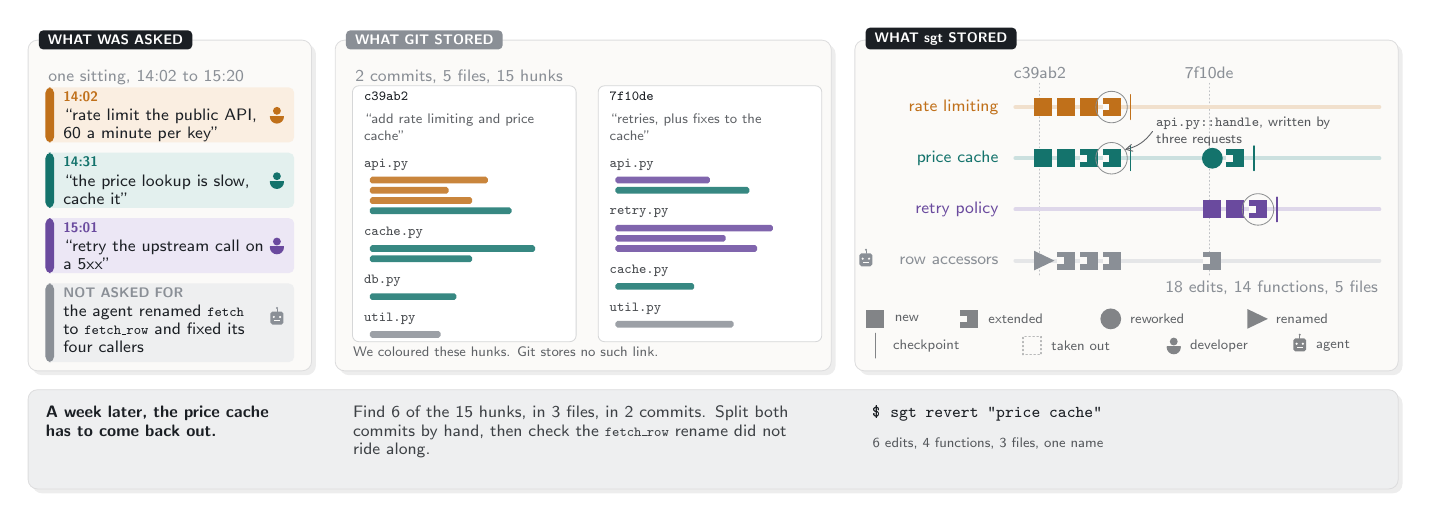
\begin{tikzpicture}[x=1mm, y=1mm, line cap=round, font=\sffamily]

% ===================== panel A: what the developer said ====================
\panel{0}{15}{36}{42}{sgtInk}{WHAT WAS ASKED}
\node[note, anchor=north west, text=sgtGrey] at (2.2,53.6) {one sitting, 14:02 to 15:20};

% #1 top y, #2 height, #3 colour, #4 wash, #5 time, #6 text
\newcommand{\reqcard}[6]{%
  \fill[#4, rounded corners=0.7mm] (2.2,{#1-#2}) rectangle (33.8,#1);
  \fill[#3, rounded corners=0.7mm] (2.2,{#1-#2}) rectangle (3.3,#1);
  \node[anchor=north west, inner sep=0, text=#3,
        font=\sffamily\bfseries\fontsize{4.9}{5.6}\selectfont] at (4.4,{#1-0.5}) {#5};
  \node[anchor=north west, text width=25.5mm, align=left, inner sep=0,
        font=\sffamily\fontsize{5.7}{6.5}\selectfont, text=sgtInk]
    at (4.4,{#1-2.7}) {#6};}

\reqcard{51.0}{7.0}{fRate}{wRate}{14:02}{``rate limit the public API, 60 a minute per key''}
\whodev{31.6}{47.5}{fRate}
\reqcard{42.7}{7.0}{fCache}{wCache}{14:31}{``the price lookup is slow, cache it''}
\whodev{31.6}{39.2}{fCache}
\reqcard{34.4}{7.0}{fRetry}{wRetry}{15:01}{``retry the upstream call on a 5xx''}
\whodev{31.6}{30.9}{fRetry}
\reqcard{26.1}{10.0}{sgtGrey}{wGrey}{NOT ASKED FOR}{the agent renamed \fsym{fetch} to \fsym{fetch\_row} and fixed its four callers}
\whoagent{31.6}{21.6}{sgtGrey}

% ===================== panel B: what git stored ============================
\panel{39}{15}{63}{42}{sgtGrey}{WHAT GIT STORED}
\node[note, anchor=north west, text=sgtGrey] at (41.2,53.6) {2 commits, 5 files, 15 hunks};

% #1 x, #2 sha, #3 message
\newcommand{\commitblock}[3]{%
  \draw[rounded corners=0.8mm, line width=0.3pt, color=sgtInk!18, fill=white]
    (#1,18.7) rectangle ({#1+28.4},51.2);
  \node[anchor=north west, inner sep=0, text=sgtInk,
        font=\ttfamily\fontsize{5.2}{6}\selectfont] at ({#1+1.4},50.5) {#2};
  \node[anchor=north west, text width=24mm, align=left, inner sep=0, text=sgtInk!70,
        font=\sffamily\fontsize{5.3}{6.1}\selectfont] at ({#1+1.4},47.7) {#3};}
% #1 x, #2 y, #3 name
\newcommand{\fname}[3]{\node[anchor=north west, inner sep=0, text=sgtInk!80,
  font=\ttfamily\fontsize{5.2}{6}\selectfont] at ({#1+1.4},#2) {#3};}

\commitblock{41.2}{c39ab2}{``add rate limiting and price cache''}
\fname{41.2}{42.0}{api.py}
  \hunk{43.4}{38.8}{15}{fRate}\hunk{43.4}{37.5}{10}{fRate}
  \hunk{43.4}{36.2}{13}{fRate}\hunk{43.4}{34.9}{18}{fCache}
\fname{41.2}{33.3}{cache.py}
  \hunk{43.4}{30.1}{21}{fCache}\hunk{43.4}{28.8}{13}{fCache}
\fname{41.2}{27.2}{db.py}
  \hunk{43.4}{24.0}{11}{fCache}
\fname{41.2}{22.4}{util.py}
  \hunk{43.4}{19.2}{9}{sgtGrey}

\commitblock{72.4}{7f10de}{``retries, plus fixes to the cache''}
\fname{72.4}{42.0}{api.py}
  \hunk{74.6}{38.8}{12}{fRetry}\hunk{74.6}{37.5}{17}{fCache}
\fname{72.4}{35.9}{retry.py}
  \hunk{74.6}{32.7}{20}{fRetry}\hunk{74.6}{31.4}{14}{fRetry}\hunk{74.6}{30.1}{18}{fRetry}
\fname{72.4}{28.5}{cache.py}
  \hunk{74.6}{25.3}{10}{fCache}
\fname{72.4}{23.7}{util.py}
  \hunk{74.6}{20.5}{15}{sgtGrey}

% the colours in this panel are the paper's, not git's, and saying so is the point
\node[anchor=north west, inner sep=0, text=sgtInk!70,
      font=\sffamily\fontsize{5.2}{6}\selectfont] at (41.2,18.1)
  {We coloured these hunks. Git stores no such link.};

% ===================== panel C: what sgt stored ===========================
\panel{105}{15}{69}{42}{sgtInk}{WHAT \textsf{sgt} STORED}

\draw[commitcol] (128.5,27.2) -- (128.5,51.6);
\draw[commitcol] (150.0,27.2) -- (150.0,51.6);
\node[note, text=sgtGrey, anchor=south] at (128.5,51.8) {c39ab2};
\node[note, text=sgtGrey, anchor=south] at (150.0,51.8) {7f10de};

\newcommand{\raillabel}[3]{\node[lbl, anchor=east, text=#3] at (123.6,#1) {#2};}
% A ring saying: this mark and the other ringed marks are the same function.
% Solid, and drawn solid on purpose. The legend two rows below this one gives a
% dotted outline to an edit that is no longer included, and every other figure
% spends dotted the same way, so a dotted ring here would mark the one fact in
% the panel that \sgt{} does record as the one thing it does not.
\newcommand{\shared}[2]{\draw[color=sgtInk!50, line width=0.3pt]
  (#1,#2) circle (2.0);}

% rate limiting
\draw[rail=fRate] (125.4,48.5) -- (171.6,48.5);
  \raillabel{48.5}{rate limiting}{fRate}
\opadd{128.9}{48.5}{fRate}\opadd{131.8}{48.5}{fRate}\opadd{134.7}{48.5}{fRate}
\opext{137.6}{48.5}{fRate}\ckpt{140.0}{48.5}{fRate}
\shared{137.6}{48.5}

% price cache
\draw[rail=fCache] (125.4,42.0) -- (171.6,42.0);
  \raillabel{42.0}{price cache}{fCache}
\opadd{128.9}{42.0}{fCache}\opadd{131.8}{42.0}{fCache}\opext{134.7}{42.0}{fCache}
\opext{137.6}{42.0}{fCache}\ckpt{140.0}{42.0}{fCache}
\oprew{150.4}{42.0}{fCache}\opext{153.3}{42.0}{fCache}\ckpt{155.7}{42.0}{fCache}
\shared{137.6}{42.0}

% retry policy
\draw[rail=fRetry] (125.4,35.5) -- (171.6,35.5);
  \raillabel{35.5}{retry policy}{fRetry}
\opadd{150.4}{35.5}{fRetry}\opadd{153.3}{35.5}{fRetry}\opext{156.2}{35.5}{fRetry}
\ckpt{158.6}{35.5}{fRetry}
\shared{156.2}{35.5}

% the rename nobody asked for
\draw[rail=sgtGrey] (125.4,29.0) -- (171.6,29.0);
  \raillabel{29.0}{row accessors}{sgtGrey}
\opmove{128.9}{29.0}{sgtGrey}\opext{131.8}{29.0}{sgtGrey}\opext{134.7}{29.0}{sgtGrey}
\opext{137.6}{29.0}{sgtGrey}\opext{150.4}{29.0}{sgtGrey}
\whoagent{106.4}{29.0}{sgtGrey}

% What the rings mean. The leader stops on the ring's own circumference rather
% than short of it, because the checkpoint tick stands where it used to land and
% an arrow between a ring and a tick names whichever of the two the reader
% happens to look at.
\annot{142.8}{45.4}{139.3}{43.1}{20}{sgtInk}
\node[anchor=west, text width=25mm, align=left, inner sep=0, text=sgtInk!75,
      font=\sffamily\fontsize{5.1}{5.9}\selectfont] at (143.2,45.4)
  {\fsym{api.py::handle}, written by three requests};

\node[note, anchor=east, text=sgtGrey] at (171.8,25.5) {18 edits, 14 functions, 5 files};

% legend, inside the panel whose marks it explains
\newcommand{\leg}[3]{\node[anchor=west, inner sep=0, text=sgtInk!70,
  font=\sffamily\fontsize{5.1}{5.9}\selectfont] at ({#1+2.4},#2) {#3};}
\opadd{107.6}{21.6}{sgtInk!55}\leg{107.6}{21.6}{new}
\opext{119.5}{21.6}{sgtInk!55}\leg{119.5}{21.6}{extended}
\oprew{137.5}{21.6}{sgtInk!55}\leg{137.5}{21.6}{reworked}
\opmove{156.0}{21.6}{sgtInk!55}\leg{156.0}{21.6}{renamed}
\ckpt{107.6}{18.2}{sgtInk!55}\leg{107.4}{18.2}{checkpoint}
\opghost{127.5}{18.2}{sgtInk!55}\leg{127.5}{18.2}{taken out}
\whodev{145.5}{18.2}{sgtInk!55}\leg{145.1}{18.2}{developer}
\whoagent{161.5}{18.2}{sgtInk!55}\leg{161.1}{18.2}{agent}

% ===================== the same task, of both records =====================
\plainpanel{0}{0}{174}{12.6}{wGrey}

\node[anchor=north west, text width=32mm, align=left, inner sep=0, text=sgtInk,
      font=\sffamily\bfseries\fontsize{6.0}{7.0}\selectfont] at (2.2,10.6)
  {A week later, the price cache has to come back out.};

\node[anchor=north west, text width=59mm, align=left, inner sep=0, text=sgtInk!85,
      font=\sffamily\fontsize{5.7}{6.7}\selectfont] at (41.2,10.6)
  {Find 6 of the 15 hunks, in 3 files, in 2 commits. Split both commits by hand,
   then check the \fsym{fetch\_row} rename did not ride along.};

\node[anchor=north west, inner sep=0, text=sgtInk,
      font=\ttfamily\fontsize{5.9}{7}\selectfont] at (107.2,10.6)
  {\$ sgt revert "price cache"};
\node[anchor=north west, inner sep=0, text=sgtInk!75,
      font=\sffamily\fontsize{5.5}{6.5}\selectfont] at (107.2,6.6)
  {6 edits, 4 functions, 3 files, one name};

\end{tikzpicture}

  \caption{\FigOneCaption}
  \Description{\FigOneDescription}
  \label{fig:two-records}
\end{teaserfigure}

\maketitle

\section{Introduction}

A version control system records changes so they can be revisited and reversed.
Every widely adopted system records lines of code---whether as
snapshots~\cite{git2026} or as patches to those
lines~\cite{roundy2005,pijul2024}---and groups them into commits a developer
names. This agreement dates to the earliest systems and has survived every
redesign since, for a reason that was sound from the start: the developer
authored the code, held at least a rough model of what changed and
why~\cite{naur1985,ko2006}, and could therefore supply the decomposition
whenever a tool asked for it. Developers now specify intent in natural language and models translate it into
edits across files~\cite{sarkar2025}. Three controlled field experiments show
this shift produces 26\% more code per week with no measurable quality
decline~\cite{cui2025}. The condition that made the agreement sound---that the
developer holds a model of what changed and why---no longer holds reliably. A
developer who types three sentences in an hour and receives fourteen functions
across five files cannot supply the decomposition a tool asks for, because they
never held it. We argue that the design choice should be renegotiated.

Three consequences of this shift make the mismatch concrete. First, the unit
that version control addresses, the line, is no longer stable enough to serve as
an anchor. A model that generates a function in one response and regenerates it
with different formatting or variable names in the next has changed every line
while changing nothing a developer would name. Across 211 million changed lines
from public repositories authored between 2020 and 2024, the share associated
with refactoring---lines moved into a better position rather than written
afresh---fell from a quarter to under a tenth, while code revised within two
weeks of being written roughly doubled~\cite{gitclear2025}. A line is now
replaced faster than it settles into a position worth recording, and the
developer wants to revisit a feature as it stood two requests ago---a unit
the line-level record cannot express.

Second, the developer does not hold a detailed model of what the code
says~\cite{sarkar2022}. A natural language prompt specifies an outcome
but not the logic that implements it, so the implementation contains decisions
the model made and the developer has not reviewed. Barke et al.\ observed
programmers reading generated code for shape rather than line by
line~\cite{barke2023}, Tang et al.\ found that developers often do not notice
which code a model wrote and delete it rather than repair it~\cite{tang2024},
and among 410 developers surveyed by Liang et al.\ understanding generated code
was one of the most frequently reported
difficulties~\cite{liang2024}. The consequence for version
control is that the developer who searches a history for a prior state must
describe it in terms they never acquired. This is the vocabulary problem Furnas
et al.\ measured in information retrieval~\cite{furnas1987}, now appearing inside
the repository. Nguyen and Glassman observed it directly: beginning programmers
and code models systematically misread each other's vocabulary, so a developer's
search terms and the model's naming choices diverge even when both refer to the
same behaviour~\cite{nguyen2024}. The developer searches with vocabulary they
never learned and finds whatever happens to match instead of the version that
served a stated purpose~\cite{codoban2015}.

Third, the unit the developer thinks in has moved from a location in the code to
a purpose the code serves. A prompt names what the software should do (rather
than which file to edit), so the developer's mental model of their own work is
organised by feature: the retry policy, the export endpoint, the rate limiter. This is the
level the program comprehension literature has always found people work at:
Biggerstaff et al.\ called recovering which functions implement a named concern
the concept assignment problem~\cite{biggerstaff1993}, and the feature location
field exists because answering it by reading code is
expensive~\cite{dit2013}. The commit is the closest unit a version control system
offers, and it does not correspond to this level, since Herzig and Zeller found
changes serving several unrelated purposes throughout the histories of five open
source Java projects~\cite{herzig2013}. An agent session produces exactly that
structure, because a commit ends where the developer stopped to type a command
and a request ends somewhere else.

The response we describe is a version control system that records at the grain
the developer thinks at. Instead of recording lines inside a commit, we parse
each file into its functions and classes~\cite{treesitter} and record one edit
per changed function, together with what that edit was built on. We group those
functions into features from how they change and how they refer to one
another~\cite{zimmermann2004,ying2004,traag2019}, and label each group with the
words the developer and the agent used while the work was happening. A version
of the code is then a set of these edits, and the files on disk are rebuilt
from whichever set is included, so a feature can be taken out or put back by
naming it rather than by naming the lines it produced. None of the individual techniques is new. Change coupling mining, community
detection, feature location, and set-based version control each have a
literature. What is new is composing them into a single tool that a developer
operates daily, because that composition introduces interactions none of the
original designs anticipated. A function identity tracker that loses a rename
breaks the dependency chain a revert depends on. A grouping inference that absorbs
a shared helper pulls unrelated work into a single feature. A layout record (the
whitespace between functions) that becomes individually addressable acquires
failure modes the entity record does not have, and 68\% of the violations we found
in ten thousand operations entered through that seam. The contribution is in making
the composition survive daily use on a real codebase, in measuring where it fails
honestly, and in reporting both the design's costs and the conditions under which
it should not be adopted.

For example, a service that answers price quotes for a trading dashboard has a
handler, a database layer, and a set of row accessors. On Monday the developer
prompts \cmd{cache the price lookup, it takes 400ms and the price barely moves},
and the agent writes \sym{cache.py::get\_cached} and \sym{cache.py::\_ttl}, gives
\sym{db.py::query} a parameter for how long a cached price stays good so the cache
can pass one through, and changes \sym{api.py::handle} to consult the cache before
the database. That is four edits to four functions in three files, and the two in
\sym{cache.py} share no line with the one in \sym{api.py}, yet all four are filed
under one name. Over the next two days two further prompts change
\sym{api.py::handle} again, one adding a rate limit and one adding a retry policy,
and while it is adding the retry the agent goes back and reworks two of the cache's
own functions, which brings the price cache to six edits. A colleague adds a metric
for quote latency. Three weeks later the developer
finds the dashboard showing a price sixty seconds stale, so they type
\cmd{sgt revert "price cache"}. \sgt{} prints the six edits that would come out,
names \sym{api.py::handle} as the one function where later work was built on
something being removed, shows the text each change would produce, and asks before
touching anything. The rate limit and the retry policy stay, because their edits
are still included; the colleague's metric stays, because it was never in the set
coming out; and the parameter leaves both \sym{db.py::query} and
\sym{api.py::handle}, because both were in it. When the developer decides a week
later that the cache was worth keeping after all, \cmd{sgt restore} returns the
files byte for byte, because putting the six edits back is the same set arithmetic
as taking them out and nothing is replayed as a patch.
Figure~\ref{fig:two-records} draws these three requests arriving in a single
sitting, under both records, and Section~\ref{sec:walkthrough} follows this
repository through five sittings.

Three prices are paid for this, all of them in the first hour of use rather than
in some later edge case. Two edits to the same function made from the same
starting point are recorded as competing versions that a person has to decide
between, including the pair at opposite ends of a fifty line function that touch
no common line and that git would have merged without comment. The grouping of
edits into named requests is inferred, so it is a guess and it will sometimes be
wrong, and correcting it costs the developer a rename, a merge, or a split, none
of which moves a recorded edit. \sgt{} reads Python, TypeScript, and TSX and
versions every other file whole, at the grain git already uses, so a repository
whose interesting logic is written in Go gets nothing from \sgt{} today.

The paper makes four contributions. We characterise the mismatch between the unit
a developer using an agent decides in and the unit a version control system
records, one attempted operation at a time (Section~\ref{sec:scenarios}), in the
style of conceptual analysis Pérez De Rosso and Jackson applied to git
itself~\cite{perezderosso2013,perezderosso2016}. We describe \sgt{}'s design as
four commitments, say what each one buys and what it costs, and run the whole set
of operations on one repository (Sections~\ref{sec:design}
and~\ref{sec:walkthrough}). We state which observation would show each of our
claims to be wrong, and pre-register the study that would produce it
(Section~\ref{sec:study}). We report what fifty-seven days of \sgt{} versioning its
own construction taught us about where the design breaks
(Section~\ref{sec:discussion}), and what three pilots taught us about the distance between a property that holds
across 10{,}237 operations and a property a new user can rely on
(Section~\ref{sec:pilot}).

\section{Related Work}
\label{sec:related}

\subsection{Programming by request}

The ways to program with foundation models have changed constantly over the last
four years, along with the advance in what the models can do. At first a model was
mostly a programming assistant offering inline code completion. Barke et al.\
watched 20 programmers and found them using it in two ways, finishing a line they
had already planned, or asking for a starting point in code they did not yet know
how to write~\cite{barke2023}. Vaithilingam et al.\ found that 24 participants
using Copilot did not complete tasks faster and still preferred to keep it on,
because it gave them a draft to work from~\cite{vaithilingam2022}, and Sarkar et
al.\ collected what the experience felt like from the developer's
side~\cite{sarkar2022}. In all of these the developer accepted a line or a block
of code. Four years later SWE-bench gives a model a natural language issue report
from a real repository and scores it on whether the repository's own tests pass
afterwards~\cite{jimenez2024}, and the systems built to score well on it edit
several files in a loop~\cite{yang2024}. The unit a developer hands over has gone
from a line to a paragraph of English, and the code that comes back is
correspondingly larger.

All of this work studies the minutes around acceptance, asking whether the code
is correct~\cite{perry2023}, whether the developer can tell that it is
correct~\cite{vasconcelos2025}, whether they trust
it~\cite{liang2024,cheng2024}, and how much faster they
finish~\cite{mozannar2024,cui2025}. But did the programmer come to understand the
codebase, understand it enough to explain why it is constructed this way rather
than only to say what it is, understand it enough to recall what their codebase
was a few weeks ago, what has changed since, and what state it is in now? We find
programmers gradually losing the theory of their own
codebase~\cite{naur1985} over the time they use these tools, losing the ability to
describe the rationale behind a design, the ability to carry out a further
modification, and the ability to recall what the codebase held. We suspect this
becomes more of a problem the further specifying in natural language can carry a
developer without their ever having to examine the code.

\subsection{What a version control system agrees to record}

Git records a version as a snapshot of the whole working tree, and each commit
names its parents plus a tree of file contents addressed by hash~\cite{git2026}.
Verifying that a history has not been altered is then a matter of rehashing it,
and a merge is computed on demand from a common ancestor, so nothing in the
repository has to say what happened when two edits met. We keep the first of those
properties and give up the second on purpose. \sgt{} addresses its records by
their contents, and when two edits to one function descend from the same parent it
records that they did rather than computing what the pair amounts to, for the
reason Section~\ref{sec:fork} gives.

Pérez De Rosso and Jackson analysed git's concepts against the purposes users
bring to them, found several places where a concept serves a purpose users do not
have, and removed the staging area and detached \cmd{HEAD} in their
redesign~\cite{perezderosso2013,perezderosso2016}. The commit survives that
redesign untouched, and it should, because it serves a purpose users do have. It
is also the smallest thing git can address, so any operation over less than a
commit works by having the developer point at lines, and \cmd{git add -p} and
\cmd{git rebase -i} are the tools for pointing. Under git's original constraints
this is the cheapest correct design available, because the person running
\cmd{git add -p} in 2005 had typed the lines minutes earlier, and writing their
decomposition into the repository would have meant maintaining a second structure
that could disagree with the first.

Darcs takes the other option and records a version as a patch that adds and
removes lines in a stated context~\cite{roundy2005}. Patches that do not depend on
each other commute, so a user can pull the third patch in a series without the
first two, and the design has been formalised and reimplemented since on a data
structure that makes the operations fast~\cite{jacobson2009,mimram2013,pijul2024}.
A Darcs user who pulls one
patch onto another branch moves the patch that was recorded, along with the
dependencies it names, where git's cherry-pick reapplies a diff in a context it
was not written against and produces a second commit with a second hash, so the
same work has two identities. But Darcs works out what a patch depends on from the
lines the patch touches, so a dependency that leaves no trace in the text goes
unrecorded. When an agent adds a \sym{Retry} class in a new file and edits
\sym{api.py::handle} to call it, the two patches share no line, and nothing in the
record says that pulling the second without the first yields a file referring to a
name that does not exist. Darcs is explicit about this and offers a way to declare
such a dependency by hand, and we would have made the same call in 2003, because
computing a dependency between two functions requires parsing the language and a
system that parses works for some languages and not for others. Darcs declined
that price and we pay it.

\begin{figure*}[t]
  \centering
  % Figure 2. The same hour of work in four records, and what one operation costs
% in each. Same session as Figure 1, same colours, same glyphs.
\newcommand{\FigTwoCaption}{One hour of work with a coding agent, recorded four
ways, with the same request removed from each. The unit a system records decides
which sets a developer can name. Git and Darcs both bottom out at a line, so
removing the caching means selecting lines. Jujutsu and Mercurial add a durable
identity above the line, and that identity belongs to a commit, so a squashed
session carries one identity for all three requests. \sgt{} records one edit per
function together with the request it was made for. The developer supplied that
request and never wrote it down.}

\newcommand{\FigTwoDescription}{A four row comparison. Each row is a card named
after a version control system, drawing the same one hour agent session in that
system's units, with the unit of record stated on the left and the cost of
removing the caching request on the right. The git row draws two commit boxes
filled with coloured diff stripes of four different colours mixed together. The
Darcs and Pijul row draws nine patch tokens in a line with arcs above joining the
patches that share lines, and one dashed arc below joining two patches that depend
on each other through a function call, marked as not recorded. The Jujutsu and
Mercurial row draws one box of mixed stripes, an arrow, and a second box of the
same mixed stripes, labelled with the same change identifier and two different
commit hashes. The sgt row draws four labelled horizontal lines, one per request,
each carrying a mark for every edit filed under that request.}

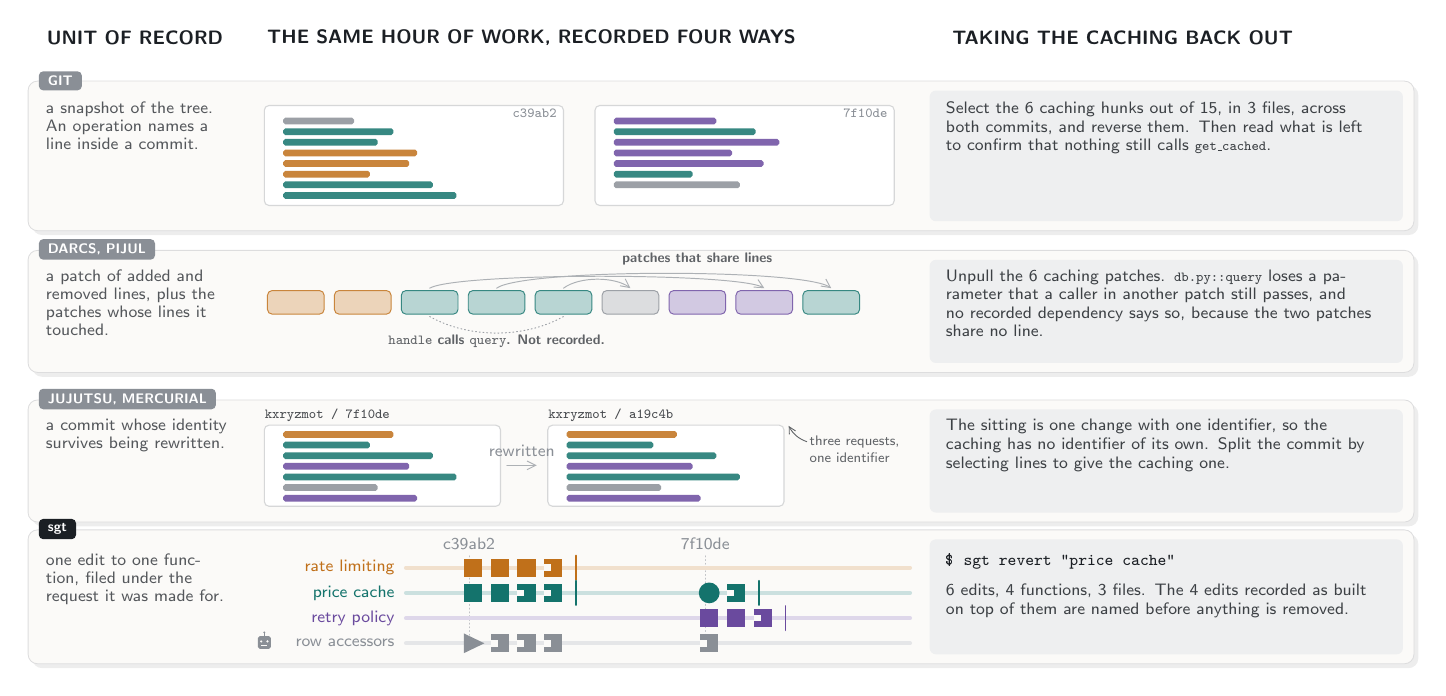
\begin{tikzpicture}[x=1mm, y=1mm, line cap=round, font=\sffamily]

% ------------------------------- headers ---------------------------------
\node[hd, anchor=west] at (2,79.5)   {UNIT OF RECORD};
\node[hd, anchor=west] at (30,79.5)  {THE SAME HOUR OF WORK, RECORDED FOUR WAYS};
\node[hd, anchor=west] at (117,79.5) {TAKING THE CACHING BACK OUT};

% Every row is one card. The cost of the operation gets a band of its own on
% the right, so the reader can read that column straight down.
% #1 y, #2 height, #3 tab colour, #4 tab text
\newcommand{\cmprow}[4]{%
  \panel{0}{#1}{176}{#2}{#3}{#4}
  \fill[wGrey, rounded corners=0.8mm] (114.5,{#1+1.2}) rectangle (174.6,{#1+#2-1.2});}
% #1 y, #2 text
\newcommand{\rowunit}[2]{%
  \node[anchor=north west, text width=23mm, align=left, inner sep=0, text=sgtInk!75,
        font=\sffamily\fontsize{5.6}{6.5}\selectfont] at (2.2,#1) {#2};}
\newcommand{\rowcost}[2]{%
  \node[anchor=north west, text width=55.5mm, align=left, inner sep=0, text=sgtInk!85,
        font=\sffamily\fontsize{5.7}{6.7}\selectfont] at (116.5,#1) {#2};}

% =============================== git =====================================
\cmprow{55}{19}{sgtGrey}{GIT}
\rowunit{71.4}{a snapshot of the tree. An operation names a line inside a commit.}
\rowcost{71.4}{Select the 6 caching hunks out of 15, in 3 files, across both
  commits, and reverse them. Then read what is left to confirm that nothing
  still calls \fsym{get\_cached}.}

\draw[card, color=sgtInk!18, fill=white] (30,58.2) rectangle (68,70.9);
\node[anchor=north east, inner sep=0, text=sgtGrey,
      font=\ttfamily\fontsize{5}{5.6}\selectfont] at (67.2,70.5) {c39ab2};
\hunk{32.4}{68.5}{9}{sgtGrey}\hunk{32.4}{67.15}{14}{fCache}
\hunk{32.4}{65.8}{12}{fCache}\hunk{32.4}{64.45}{17}{fRate}
\hunk{32.4}{63.1}{16}{fRate}\hunk{32.4}{61.75}{11}{fRate}
\hunk{32.4}{60.4}{19}{fCache}\hunk{32.4}{59.05}{22}{fCache}

\draw[card, color=sgtInk!18, fill=white] (72,58.2) rectangle (110,70.9);
\node[anchor=north east, inner sep=0, text=sgtGrey,
      font=\ttfamily\fontsize{5}{5.6}\selectfont] at (109.2,70.5) {7f10de};
\hunk{74.4}{68.5}{13}{fRetry}\hunk{74.4}{67.15}{18}{fCache}
\hunk{74.4}{65.8}{21}{fRetry}\hunk{74.4}{64.45}{15}{fRetry}
\hunk{74.4}{63.1}{19}{fRetry}\hunk{74.4}{61.75}{10}{fCache}
\hunk{74.4}{60.4}{16}{sgtGrey}

% ========================== Darcs and Pijul ==============================
\cmprow{37}{15.5}{sgtGrey}{DARCS, PIJUL}
\rowunit{50.1}{a patch of added and removed lines, plus the patches whose lines
  it touched.}
\rowcost{50.1}{Unpull the 6 caching patches. \fsym{db.py::query} loses a
  parameter that a caller in another patch still passes, and no recorded
  dependency says so, because the two patches share no line.}

% #1 x centre, #2 colour
\newcommand{\patchtok}[2]{%
  \draw[card, color=#2!85, fill=#2!30, line width=0.35pt]
    ({#1-3.6},44.4) rectangle ({#1+3.6},47.4);}
\patchtok{34}{fRate}\patchtok{42.5}{fRate}\patchtok{51}{fCache}\patchtok{59.5}{fCache}
\patchtok{68}{fCache}\patchtok{76.5}{sgtGrey}\patchtok{85}{fRetry}\patchtok{93.5}{fRetry}
\patchtok{102}{fCache}

\draw[dep] (59.5,47.7) .. controls (63,50.2) and (98.5,50.2) .. (102,47.7);
\draw[dep] (51,47.7) .. controls (54.5,49.7) and (90,49.7) .. (93.5,47.7);
\draw[dep] (68,47.7) .. controls (70,49.2) and (74.5,49.2) .. (76.5,47.7);
\node[acc=sgtInk!70, anchor=south] at (85,50.2) {patches that share lines};
\draw[color=sgtGrey!85, line width=0.35pt, densely dotted]
  (51,44.1) .. controls (56.0,41.3) and (63.0,41.3) .. (68,44.1);
\node[acc=sgtInk!70, anchor=north] at (59.5,42.1)
  {\fsym{handle} calls \fsym{query}. Not recorded.};

% ======================= Jujutsu and Mercurial ===========================
\cmprow{18}{15.5}{sgtGrey}{JUJUTSU, MERCURIAL}
\rowunit{31.1}{a commit whose identity survives being rewritten.}
\rowcost{31.1}{The sitting is one change with one identifier, so the caching has
  no identifier of its own. Split the commit by selecting lines to give the
  caching one.}

\newcommand{\jjbox}[2]{%
  \draw[card, color=sgtInk!18, fill=white] (#1,20.0) rectangle ({#1+30},30.3);
  \hunk{{#1+2.4}}{28.7}{14}{fRate}\hunk{{#1+2.4}}{27.35}{11}{fCache}
  \hunk{{#1+2.4}}{26.0}{19}{fCache}\hunk{{#1+2.4}}{24.65}{16}{fRetry}
  \hunk{{#1+2.4}}{23.3}{22}{fCache}\hunk{{#1+2.4}}{21.95}{12}{sgtGrey}
  \hunk{{#1+2.4}}{20.6}{17}{fRetry}
  \node[anchor=south west, inner sep=0, text=sgtInk!80,
        font=\ttfamily\fontsize{5.2}{6}\selectfont] at (#1,30.7) {#2};}
\jjbox{30}{kxryzmot / 7f10de}
\jjbox{66}{kxryzmot / a19c4b}
\draw[dep] (60.8,25.2) -- (64.6,25.2);
\node[note, anchor=south, text=sgtGrey] at (62.7,25.9) {rewritten};
\annot{98.9}{28.2}{96.6}{30.2}{20}{sgtInk}
\node[anchor=north west, text width=13mm, align=left, inner sep=0, text=sgtInk!70,
      font=\sffamily\fontsize{5.2}{6}\selectfont] at (99.2,29.0)
  {three requests,\\one identifier};

% ================================= sgt ===================================
\cmprow{0}{17}{sgtInk}{\textsf{sgt}}
\rowunit{14.0}{one edit to one function, filed under the request it was made
  for.}
\node[anchor=north west, inner sep=0, text=sgtInk,
      font=\ttfamily\fontsize{5.9}{7}\selectfont] at (116.5,14.0)
  {\$ sgt revert "price cache"};
\node[anchor=north west, text width=55.5mm, align=left, inner sep=0, text=sgtInk!85,
      font=\sffamily\fontsize{5.7}{6.7}\selectfont] at (116.5,10.2)
  {6 edits, 4 functions, 3 files. The 4 edits recorded as built on top of them
   are named before anything is removed.};

\draw[commitcol] (56,2.2) -- (56,14.0);
\draw[commitcol] (86,2.2) -- (86,14.0);
\node[note, text=sgtGrey, anchor=south] at (56,14.1) {c39ab2};
\node[note, text=sgtGrey, anchor=south] at (86,14.1) {7f10de};

\newcommand{\srail}[3]{%
  \draw[rail=#3] (48,#1) -- (112,#1);
  \node[anchor=east, inner sep=0, text=#3,
        font=\sffamily\fontsize{5.8}{6.6}\selectfont] at (46.6,#1) {#2};}
\srail{12.2}{rate limiting}{fRate}
\opadd{56.5}{12.2}{fRate}\opadd{59.9}{12.2}{fRate}\opadd{63.3}{12.2}{fRate}
\opext{66.7}{12.2}{fRate}\ckpt{69.6}{12.2}{fRate}
\srail{9.0}{price cache}{fCache}
\opadd{56.5}{9.0}{fCache}\opadd{59.9}{9.0}{fCache}\opext{63.3}{9.0}{fCache}
\opext{66.7}{9.0}{fCache}\ckpt{69.6}{9.0}{fCache}
\oprew{86.5}{9.0}{fCache}\opext{89.9}{9.0}{fCache}\ckpt{92.8}{9.0}{fCache}
\srail{5.8}{retry policy}{fRetry}
\opadd{86.5}{5.8}{fRetry}\opadd{89.9}{5.8}{fRetry}\opext{93.3}{5.8}{fRetry}
\ckpt{96.2}{5.8}{fRetry}
\srail{2.6}{row accessors}{sgtGrey}
\whoagent{30.0}{2.6}{sgtGrey}
\opmove{56.5}{2.6}{sgtGrey}\opext{59.9}{2.6}{sgtGrey}\opext{63.3}{2.6}{sgtGrey}
\opext{66.7}{2.6}{sgtGrey}\opext{86.5}{2.6}{sgtGrey}

\end{tikzpicture}

  \Description{\FigTwoDescription}
  \caption{\FigTwoCaption}
  \label{fig:granularity}
\end{figure*}

Jujutsu and Mercurial both add a record of history's own history. Jujutsu gives
each change an identifier separate from its commit hash, so rewriting a commit
produces a new commit while the change keeps its name, and a change with more than
one visible commit is called divergent~\cite{jjglossary2026,jujutsu2026}.
Mercurial stores obsolescence markers apart from changeset data, keeping a history
of how the history was edited alongside the history of how the files
were~\cite{mercurial2026}. Both designs let
a developer say ``the change I was working on yesterday'' after five rebases and
be understood, and both let two people rewrite the same region of history and have
the disagreement recorded rather than silently resolved, which is the construction
\sgt{} uses for two competing versions of one function. We part company on what
receives the durable identity. In both systems it is a commit, so the identity is
exactly as coarse as the commit, and after a developer squashes a two-hour agent
session into one commit, one change identifier covers all three requests and
nothing smaller has a name. Figure~\ref{fig:granularity} puts these records beside
each other.

\subsection{Version control that already knew about functions}

Recording a version at the grain of a function has been built before, more than
once, and the reason none of it displaced the commit is the reason we think it can
now. Historage rewrites a Java repository so that every method sits in a file of
its own, at which point git's existing machinery gives each method a history of
its own~\cite{hata2011}, and FinerGit refines that format so that git's rename
detection keeps working when a method moves~\cite{higo2020}. Stellation and Coven
made the fine-grained unit the thing the repository stores rather than a
transformation applied to it, so a developer could check out a single
method~\cite{chucarroll2002,chucarroll2000}. MolhadoRef settled the problem
Section~\ref{sec:identity} reports as our weakest link, by having the development
environment record each refactoring as the developer performed it, so a rename
entered the history as an operation instead of arriving as something a later tool
had to guess at~\cite{dig2007}. Mylyn recorded, for each task a developer worked
on, the set of program elements they touched while working on it, and used that set
to decide what the environment showed them~\cite{kersten2006}. All of this existed
at least fifteen years before the first coding agent and all of it worked.
Historage and FinerGit are in use today as instruments for mining software
histories, which is research reading a repository from the outside, and a working
programmer choosing what to run on Monday morning uses none of it.

We do not read that as a failure of engineering, because a finer grain buys a
developer only what they cannot already supply for themselves, and until recently
they could supply all of it. Whoever wanted the caching out of a 2010 repository
had written the caching, so a system that told them which methods it touched was
performing work they had already done, at the price of a repository their
colleagues could not clone with plain git. What has changed is not the value of
the grain but the identity of the author, and a record that was redundant while
the developer wrote the lines is the only surviving copy of the decomposition once
they have stopped writing them. Mylyn's task context and \sgt{}'s named group of
edits are the same object built for two different situations, and the difference is
that Mylyn watched a developer's attention move through code that developer was
writing, whereas the attention \sgt{} reconstructs belonged to a process that has
already exited.

The merge question in this literature was approached from the end opposite to ours.
Horwitz, Prins and Reps showed that two versions of a program can be integrated
automatically when a semantic analysis proves the changes do not
interfere~\cite{horwitz1989}, and Apel et al.'s semistructured merge parses a file
far enough to see that two edits landed in different methods, resolving a large
share of what a line-based merge reports as a conflict~\cite{apel2011}. The design
here rests directly on two further results from that area, that a merge of the
recorded operations tells a developer more than a merge of the states those
operations produced~\cite{lippe1992}, and that a version is usefully treated as a
set with a logic over it, which is the construction Section~\ref{sec:sets}
uses~\cite{zeller1997}. \sgt{} departs from Horwitz and from Apel deliberately.
Where semistructured merge combines two edits to one
method as soon as it can see they touch different lines, \sgt{} stops and asks a
person, and Section~\ref{sec:forkoff} concedes that a repository with one person in
it is the wrong place to have tested that rule.

\subsection{Recovering a decomposition after the fact}

Commits that address more than one concern distort the tools built from a history.
Herzig and Zeller examined five open source Java projects, found such commits
throughout them, and showed that separating those changes alters which files a
defect prediction model identifies as the most likely to contain
bugs~\cite{herzig2013,herzig2016}. The untangling tools built after that finding
recover the grouping from the diff itself, partitioning it by the definition and
use relationships between the changed statements~\cite{barnett2015} or by a
dependency graph across the versions a commit spans~\cite{partachi2020}, and every
one of them is evaluated on whether it reproduces a grouping a human labelled. Two
anticipate the move we make: Dias et al.\ read the fine-grained edit events an IDE
records while the developer is still typing~\cite{dias2015}, and Shen et al.\ hand
the partition back to the developer to correct, which is the arrangement
Section~\ref{sec:names} adopts~\cite{shen2021,tao2015,wang2019}. What none of them could
assume is a statement of the boundary written down before the code existed, because
in 2015 no such statement existed to be had, and the strength of their inference is
a measure of how much they had to recover without one.

That is the loosened constraint, and it is worth being exact about what it buys,
because \sgt{} performs the same inference they do and performs it no better; we
would expect it to be worse, since it has to finish while a developer waits. What
has changed is what the inference is for. Their partition has to be right, because
it is the answer. Ours has to be close enough that a name attaches to the right
set, and the developer who reads a wrong name fixes it with a rename that moves no
code.

\sgt{} does depend on two results from this literature. Keeping a function's
identity when it is renamed or moved is the problem that refactoring detection and
tree differencing address~\cite{tsantalis2018,falleri2014,fluri2007}, and it is
the weakest link in our implementation, since a rename we fail to detect appears
as one function removed and another added. Grouping edits into features is a
clustering over which functions change together and which call each other, both
halves of which the co-change mining literature
established~\cite{zimmermann2004,ying2004,kim2005,godfrey2005}, resolved with a
community detection algorithm~\cite{traag2019,traag2011}. Both are inferences, and
Section~\ref{sec:design} states what a developer does when they are wrong.

\subsection{Histories the editor keeps}

A second tradition puts the record in the editor and asks nothing of the
developer. Azurite stores a programmer's editing operations at a finer grain than
any commit and lets them undo one past edit while keeping the edits made after
it~\cite{yoon2015,yoon2013,yoon2014}. Variolite lets a data
scientist wrap a region of code as a variant and switch between variants in place,
after Kery et al.\ found that people doing exploratory work avoid version
control for exactly that work~\cite{kery2017}, and the same tradition has held
alternative versions side by side, replayed a document's editing history, versioned
one experiment at a time, and cleaned a notebook up afterwards, in every case
recording what the developer did as a byproduct of their doing it and never asking
them to prepare
it~\cite{hartmann2008,terry2004,grossman2010,mikami2017,kery2018,head2019}. That
commitment \sgt{} keeps. All of them also stop at
the boundary of one machine: the history lives in the editor's own store, so a
colleague, a build, and a code review never see it, and the unit is a single edit
event, so a set of related edits still has no name a person can use. \sgt{} pays
for crossing that boundary by writing its record into the git repository as files
committed with the code, and Section~\ref{sec:colleague} describes what that costs.

\subsection{Layers over git built for the way people work now}

The tools developers reach for today accept git's storage and add a layer above
it. GitButler keeps several branches applied to one working directory at once,
draws each as a vertical lane with its own staging area, and lets the developer
drag a change into the lane it belongs to~\cite{gitbutler2026}, on the correct
reasoning that which branch a piece of work belongs to is easiest to decide once
the work exists. GitButler assigns an individual file change to a lane, so it
cannot express the case at the centre of Figure~\ref{fig:two-records}, where three
requests all edited \sym{api.py::handle} and no assignment of \sym{api.py} to one
lane is right. Graphite and GitHub's stacked pull requests take the ordered series
as their unit, keeping a chain of changes consistent by rebasing and retargeting
the higher layers when a lower one merges and landing every unmerged layer beneath
the topmost ready one in a single
operation~\cite{graphite2026,githubstacked2026}, which is the right answer to a
reviewer who cannot read one large change with the care they can give to each of
five small ones. Graphite's guide states the precondition plainly, that developers
must understand how to break down their work into small, incremental changes, and
every command the tool offers operates on a decomposition the developer has
already performed. In an agent session that decomposition exists in the
developer's request history and nowhere in the code.

The closest system to ours is sem, which parses about 32 languages with
tree-sitter and reports which functions, methods and classes a commit changed,
resolving an entity's identity across versions in three passes, by exact
identifier, by a structural hash that ignores whitespace and comments, and by
token overlap above 80\%~\cite{sem2026}. sem keeps its answers in a derived SQLite
cache outside the
repository, and that placement makes sem safe to adopt and safe to abandon, gives
entity-level answers about a history recorded years before sem existed, and
requires agreement from nobody else on the team. It also bounds what sem can
offer: a record any teammate's ordinary commit can silently invalidate cannot be
the record an operation acts on, so every sem command reports and none of them
changes state, and a developer who learns from \cmd{sem diff} that
\sym{get\_cached} changed removes it with a line-level tool.
\sgt{} commits its record to the repository in
order to act on it, and we pay for that in two places. A record that operations
depend on has to be repaired when it is wrong, which
Section~\ref{sec:unreproducible} reports the current cost of, and everybody who
pulls the repository now carries a record they did not ask for, which
Section~\ref{sec:colleague} works through from the point of view of the three
people who never installed \sgt{}. sem chose the safer placement and we chose the
more useful one, and the honest form of that sentence is that we have taken on an
obligation sem does not have.

\section{Five Operations a Developer Cannot Name}
\label{sec:scenarios}

The five scenarios below come from our own use of \sgt{} while building it and from
watching colleagues work with coding agents on repositories we maintain. Each one
is an operation a developer tried to perform, stated in the words they used, and
all five fail for the same reason, that the developer names the work by the request
that produced it, because that is the level their theory of the codebase is pitched
at~\cite{naur1985}, while the record they have to operate through holds lines inside
commits (Figure~\ref{fig:granularity}). Every scenario has a workaround and all the
workarounds work, so the argument is about what the workarounds cost, and what they
cost is working out from the code which function served which request, a division the
developer stated in advance and nothing wrote down.

\subsection{``Commit this when it is done, and I do not know yet when that is''}

A developer working through an agent still has to choose when to commit, and in
this hour every moment available to them is wrong in a different way. Committing
after each request writes a version of \sym{api.py::handle} into the permanent
history that existed for twenty-nine minutes and that nobody ever ran the test
suite against, and it files the agent's rework of the cache under the retry commit,
because the agent did that rework while adding the retry. Committing once at the
end produces one commit holding all three requests and the rename, and this
developer split the difference by committing twice, which is the pair
Figure~\ref{fig:two-records} draws, each of them mixing two requests with the
rename. Staging hunk by hunk produces four clean
commits and asks the developer to decide, for each of fifteen hunks, which of those
four purposes it serves. Green and Petre named the first two costs premature
commitment, where a notation forces a decision before the information it needs
exists, and the third viscosity, the resistance a notation puts up once a decision
turns out to be wrong~\cite{green1996,blackwell2003}. Git asks for the
decomposition at the moment of writing, and in a session driven by requests the
boundary does exist at that moment: what the developer lacks is not the boundary,
which they stated themselves before any of the code existed, but the list of
functions on either side of it, which only the agent ever had.

\smallskip\noindent\emph{The operation.} Record the boundary the developer already
stated, without asking them to state it a second time in a different notation.

\subsection{``Change the rate limiter I built yesterday''}

The rate limiting from 14:02 used a fixed one-minute window, and three days later
it needs a sliding one. The work lands in two of the four functions the original
request produced, and the developer's first question is what the rate limiting
looked like before they touched it. Git can follow one function at a time:
\cmd{git log -L :handle:api.py} follows a function by matching a name pattern and
\cmd{git log -S} finds the commits where a string appeared or disappeared, so the
developer runs the first command four times, once per function they believe was
involved, and assembles the four answers themselves. The set has no name, so
nothing checks whether four was the right number. Codoban et al.\ asked developers
why they examine history and found the most common reason to be understanding the
rationale behind a piece of code~\cite{codoban2015}, and LaToza and Myers found
questions about why code is the way it is among the hardest developers report
answering~\cite{latoza2010}. The rationale in this case was one sentence of
English, typed three days ago into a window that is now closed.

\smallskip\noindent\emph{The operation.} Name the work one request produced, see
its current state and its previous state, and change it as a unit.

\subsection{``Take the caching back out and leave the rest alone''}

The caching turned out to serve a stale price for up to sixty seconds, and it has
to go. Its six edits are spread over three files and two commits, mixed with nine
hunks belonging to three other purposes, one of them adds a parameter to
\sym{db.py::query} while another passes it from \sym{api.py::handle}, and three
functions the rename rewrote afterwards call a helper the caching introduced.
\cmd{git revert} takes back a whole commit, so reverting either of these two
removes work the developer is keeping. The developer therefore checks out both
commits, selects the six hunks by hand, reverses them, and then confirms that
removing the parameter did not break \sym{handle} and that the three functions the
rename rewrote no longer call \sym{get\_cached}. The confirmation takes the time,
because the record contains no statement that the \sym{db.py::query} signature and
the \sym{handle} call site were changed for the same reason.

\smallskip\noindent\emph{The operation.} Remove a named set of edits, leave every
other edit to the same files in place, and name the code that still depends on the
removed set before anything is applied.

\subsection{``Send just the export work to the release branch''}

An export endpoint has to ship today, and it was written on a branch that also
carries a half finished retry policy. \cmd{git cherry-pick} moves a commit, and the
export work is two functions in a commit that also carries part of that retry
policy, so the usual answer is a temporary branch and an interactive rebase
that splits that commit, and the split has to be done again if more export work
arrives before the release. Darcs solves the part of this that is about lines,
since a Darcs patch carries the dependencies it was recorded with and moving it
involves no reapplication (Section~\ref{sec:related}). But the export code calls a
helper the rate limiter introduced, no line-level record states that call, and the
developer finds out when the release branch fails to import.

\smallskip\noindent\emph{The operation.} Carry a named set of edits and its
dependencies to another branch, and be told before the operation which dependencies
would come along.

\subsection{``Let someone review the rate limiter while I keep building on it''}

The rate limiter was finished at 14:30 and the caching that followed calls
\sym{api.py::\_bucket}, so the two form a stack of two layers with the rate limiter
underneath. Submitting them that way required the rate limiter to be on its own
branch at 14:30, which required knowing at 14:30 that the caching would build on
it. Stacked pull requests exist because review works best on small changes arriving
often~\cite{rigby2013} and because a reviewer's main difficulty is understanding
the change in front of them~\cite{bacchelli2013}, and Graphite and GitHub automate
every step after the decision, including rebasing the upper layer when a reviewer
asks for a change to the lower one (Section~\ref{sec:related}). The decision itself
belongs to the developer and has to be made before the work exists, and in an agent
session the layering becomes visible only once both layers are written. Green and
Petre's framework has a name for this, the hidden dependency, a relationship the
system relies on that the notation does not show, and Church et al.\ traced its
effects through version control in particular~\cite{green1996,church2014}. The
notation here is the branch, and a
branch says nothing about which functions call which.

\smallskip\noindent\emph{The operation.} Discover the layering after the work
exists, and submit one layer while continuing to work on the layer above it.

\subsection{What the five have in common}

Every one of these operations takes a set of edits as its argument, and the
developer identifies that set by the purpose the edits served. Git expresses a set
of lines, a set of files, and a set of commits, and a developer can build all five
operations out of those three. The price of building them is recovering a
decomposition that nobody recorded, and that recovery stayed affordable for as long
as the person paying it was the person who had written the code.
Section~\ref{sec:design} describes what we changed so that a developer can type the
argument these five operations want.

\section{What \sgt{} Commits To}
\label{sec:design}

\begin{figure*}[t]
  \centering
  % Figure 3. The whole model in one picture: what a save writes, what a version
% is, and where the bytes in your files come from. Same session as Figure 1.
\newcommand{\FigThreeCaption}{What one save writes down, what a version is, and
where the bytes in a file come from. A save writes
one record per changed function and files the records under a guess at the request
they served, which the developer corrects with one command (left). A version is
the set of those records, so taking out the price cache is subtracting six records
from eighteen, and two rules decide which sets are allowed (middle). The files are
rebuilt from the set with the text between functions kept exactly, so the same set
always produces the same bytes (right). Two kinds of mark in the right-hand column
are the two consequences \sgt{} reports about this revert and does not act on. The hollow
triangle on \protect\fsym{api.py::handle} means the retry policy edited that
function after the cache did, so \sgt{} took the cache's lines back out of the
current text and the developer's test suite decides whether the result stands. The
open circles are three functions that still call
\protect\fsym{cache.py::get\_cached}, which \sgt{} names and leaves alone.
\protect\fsym{db.py::query} is the one function that goes back to text it had
earlier in the day.}

\newcommand{\FigThreeDescription}{Three panels. The left panel shows a terminal
transcript of one save command, followed by the three feature groups the save
landed in, one of them newly created and unnamed, and then a card listing the
five fields one edit record holds. The middle panel lists the fourteen functions
this session changed, grouped by file, with the edit marks for each on a short
rail, in two columns. The left column is the set as it stands and the right
column is the same list after the price cache has been reverted, where the cache
edits are drawn as dotted outlines, one file is marked as removed, one function is
marked with a hollow triangle, and three functions are marked with an open circle.
The right panel draws the file
api.py twice as a vertical stack of bands, once before and once after, where
coloured bands are function bodies and grey bands are the text between them,
which is identical in both.}

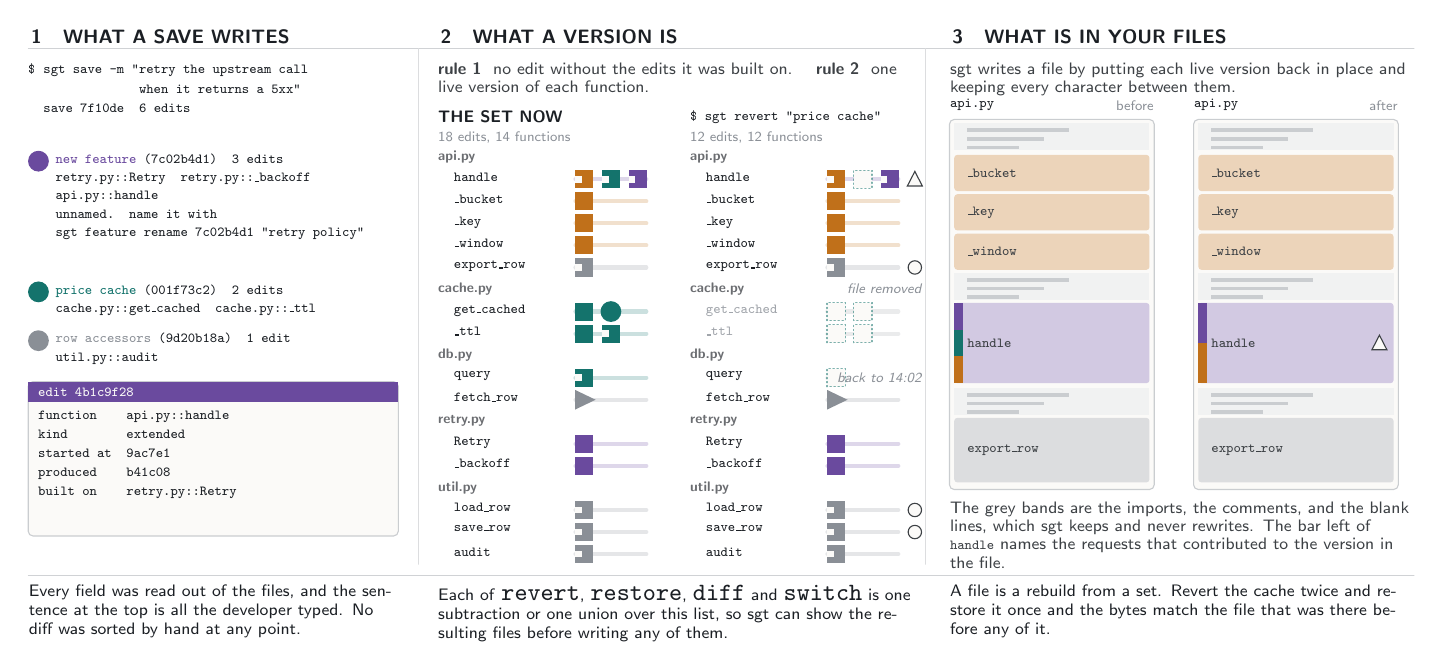
\begin{tikzpicture}[x=1mm, y=1mm, line cap=round, font=\sffamily]

\node[hd, anchor=west] at (0,78)   {1\quad WHAT A SAVE WRITES};
\node[hd, anchor=west] at (52,78)  {2\quad WHAT A VERSION IS};
\node[hd, anchor=west] at (117,78) {3\quad WHAT IS IN YOUR FILES};
\draw[color=sgtGrey!40, line width=0.3pt] (0,76.5) -- (176,76.5);
\draw[color=sgtGrey!30, line width=0.3pt] (49.5,11) -- (49.5,76.5);
\draw[color=sgtGrey!30, line width=0.3pt] (114,11) -- (114,76.5);
\draw[color=sgtGrey!40, line width=0.3pt] (0,9.6) -- (176,9.6);

% ==================== panel 1: what a save writes =========================
\node[anchor=north west, align=left, inner sep=0, text=sgtInk,
      font=\ttfamily\fontsize{5.2}{7}\selectfont] at (0,74.6)
  {\$ sgt save -m "retry the upstream call\\
   \hphantom{\$ sgt save -m "}when it returns a 5xx"\\
   \ \ save 7f10de\ \ 6 edits};

\oprew{1.3}{62.2}{fRetry}
\node[anchor=north west, align=left, inner sep=0, text=sgtInk,
      font=\ttfamily\fontsize{5.2}{6.6}\selectfont] at (3.4,63.2)
  {\textcolor{fRetry}{new feature} (7c02b4d1)\ \ 3 edits\\
   retry.py::Retry\ \ retry.py::\_backoff\\
   api.py::handle\\
   unnamed. name it with\\
   sgt feature rename 7c02b4d1 "retry policy"};

\oprew{1.3}{45.6}{fCache}
\node[anchor=north west, align=left, inner sep=0, text=sgtInk,
      font=\ttfamily\fontsize{5.2}{6.6}\selectfont] at (3.4,46.6)
  {\textcolor{fCache}{price cache} (001f73c2)\ \ 2 edits\\
   cache.py::get\_cached\ \ cache.py::\_ttl};

\oprew{1.3}{39.4}{sgtGrey}
\node[anchor=north west, align=left, inner sep=0, text=sgtInk,
      font=\ttfamily\fontsize{5.2}{6.6}\selectfont] at (3.4,40.4)
  {\textcolor{sgtGrey}{row accessors} (9d20b18a)\ \ 1 edit\\
   util.py::audit};

% one record, in full
\draw[card, color=sgtGrey!45, fill=sgtPaper] (0,14.6) rectangle (47,34.2);
\fill[fRetry] (0,31.6) rectangle (47,34.2);
\node[anchor=west, inner sep=0, text=sgtPaper,
      font=\ttfamily\fontsize{5.2}{6}\selectfont] at (1.2,32.9) {edit 4b1c9f28};
\node[anchor=north west, align=left, inner sep=0, text=sgtInk,
      font=\ttfamily\fontsize{5.2}{6.9}\selectfont] at (1.2,30.6)
  {function\ \ \ \ api.py::handle\\
   kind\ \ \ \ \ \ \ \ extended\\
   started at\ \ 9ac7e1\\
   produced\ \ \ \ b41c08\\
   built on\ \ \ \ retry.py::Retry};

% ==================== panel 2: what a version is ==========================
\node[anchor=north west, align=left, text width=61mm, inner sep=0, text=sgtInk!85,
      font=\sffamily\fontsize{5.6}{6.6}\selectfont] at (52,74.8)
  {\textbf{rule 1}\ \ no edit without the edits it was built on.\ \ \ \
   \textbf{rule 2}\ \ one live version of each function.};

\node[anchor=north west, align=left, inner sep=0, text=sgtInk,
      font=\sffamily\bfseries\fontsize{5.6}{6.4}\selectfont] at (52,68.6)
  {THE SET NOW};
\node[anchor=north west, inner sep=0, text=sgtGrey,
      font=\sffamily\fontsize{5.2}{6}\selectfont] at (52,66.0)
  {18 edits, 14 functions};
\node[anchor=north west, align=left, inner sep=0, text=sgtInk,
      font=\ttfamily\fontsize{5.4}{6.2}\selectfont] at (84,68.6)
  {\$ sgt revert "price cache"};
\node[anchor=north west, inner sep=0, text=sgtGrey,
      font=\sffamily\fontsize{5.2}{6}\selectfont] at (84,66.0)
  {12 edits, 12 functions};

% #1 x, #2 y, #3 file name
\newcommand{\FTfile}[3]{\node[anchor=north west, inner sep=0, text=sgtInk!65,
  font=\sffamily\bfseries\fontsize{5.2}{6}\selectfont] at (#1,#2) {#3};}
% #1 x, #2 y, #3 symbol name, #4 colour
\newcommand{\FTsym}[4]{\node[anchor=north west, inner sep=0, text=#4,
  font=\ttfamily\fontsize{5.2}{6}\selectfont] at (#1,#2) {#3};}
% a hollow up-triangle: this version was re-drafted, and the tests decide
\newcommand{\FTredraft}[2]{\draw[sgtInk!85, line width=0.4pt, fill=sgtPaper]
  ({#1-0.95},{#2-0.85}) -- ({#1+0.95},{#2-0.85}) -- (#1,{#2+1.0}) -- cycle;}
% an open circle: this function still calls something the revert removed
\newcommand{\FTcalls}[2]{\draw[sgtInk!85, line width=0.4pt, fill=sgtPaper]
  (#1,#2) circle (0.85);}
% #1 x of rail start, #2 y of rail
\newcommand{\FTrail}[3]{\draw[rail=#3] (#1,#2) -- ({#1+9},#2);}
\newcommand{\FTraildim}[2]{\draw[raildim] (#1,#2) -- ({#1+9},#2);}

% ---- left column: the set as it stands
\FTfile{52}{63.6}{api.py}
\FTsym{54}{60.8}{handle}{sgtInk}
  \FTrail{69.5}{59.9}{fRetry}
  \opext{70.6}{59.9}{fRate}\opext{74.0}{59.9}{fCache}\opext{77.4}{59.9}{fRetry}
\FTsym{54}{58.0}{\_bucket}{sgtInk}
  \FTrail{69.5}{57.1}{fRate}\opadd{70.6}{57.1}{fRate}
\FTsym{54}{55.2}{\_key}{sgtInk}
  \FTrail{69.5}{54.3}{fRate}\opadd{70.6}{54.3}{fRate}
\FTsym{54}{52.4}{\_window}{sgtInk}
  \FTrail{69.5}{51.5}{fRate}\opadd{70.6}{51.5}{fRate}
\FTsym{54}{49.6}{export\_row}{sgtInk}
  \FTrail{69.5}{48.7}{sgtGrey}\opext{70.6}{48.7}{sgtGrey}
\FTfile{52}{46.8}{cache.py}
\FTsym{54}{44.0}{get\_cached}{sgtInk}
  \FTrail{69.5}{43.1}{fCache}
  \opadd{70.6}{43.1}{fCache}\oprew{74.0}{43.1}{fCache}
\FTsym{54}{41.2}{\_ttl}{sgtInk}
  \FTrail{69.5}{40.3}{fCache}
  \opadd{70.6}{40.3}{fCache}\opext{74.0}{40.3}{fCache}
\FTfile{52}{38.4}{db.py}
\FTsym{54}{35.6}{query}{sgtInk}
  \FTrail{69.5}{34.7}{fCache}\opext{70.6}{34.7}{fCache}
\FTsym{54}{32.8}{fetch\_row}{sgtInk}
  \FTrail{69.5}{31.9}{sgtGrey}\opmove{70.6}{31.9}{sgtGrey}
\FTfile{52}{30.0}{retry.py}
\FTsym{54}{27.2}{Retry}{sgtInk}
  \FTrail{69.5}{26.3}{fRetry}\opadd{70.6}{26.3}{fRetry}
\FTsym{54}{24.4}{\_backoff}{sgtInk}
  \FTrail{69.5}{23.5}{fRetry}\opadd{70.6}{23.5}{fRetry}
\FTfile{52}{21.6}{util.py}
\FTsym{54}{18.8}{load\_row}{sgtInk}
  \FTrail{69.5}{17.9}{sgtGrey}\opext{70.6}{17.9}{sgtGrey}
\FTsym{54}{16.0}{save\_row}{sgtInk}
  \FTrail{69.5}{15.1}{sgtGrey}\opext{70.6}{15.1}{sgtGrey}
\FTsym{54}{13.2}{audit}{sgtInk}
  \FTrail{69.5}{12.3}{sgtGrey}\opext{70.6}{12.3}{sgtGrey}

% ---- right column: the same list, six edits subtracted
\FTfile{84}{63.6}{api.py}
\FTsym{86}{60.8}{handle}{sgtInk}
  \FTrail{101.5}{59.9}{fRetry}
  \opext{102.6}{59.9}{fRate}\opghost{106.0}{59.9}{fCache}\opext{109.4}{59.9}{fRetry}
  \FTredraft{112.6}{59.9}
\FTsym{86}{58.0}{\_bucket}{sgtInk}
  \FTrail{101.5}{57.1}{fRate}\opadd{102.6}{57.1}{fRate}
\FTsym{86}{55.2}{\_key}{sgtInk}
  \FTrail{101.5}{54.3}{fRate}\opadd{102.6}{54.3}{fRate}
\FTsym{86}{52.4}{\_window}{sgtInk}
  \FTrail{101.5}{51.5}{fRate}\opadd{102.6}{51.5}{fRate}
\FTsym{86}{49.6}{export\_row}{sgtInk}
  \FTrail{101.5}{48.7}{sgtGrey}\opext{102.6}{48.7}{sgtGrey}
  \FTcalls{112.6}{48.7}
\FTfile{84}{46.8}{cache.py}
\node[anchor=east, inner sep=0, text=sgtGrey,
      font=\sffamily\itshape\fontsize{5}{5.8}\selectfont] at (113.5,46.0)
  {file removed};
\FTsym{86}{44.0}{get\_cached}{sgtGrey!80}
  \FTraildim{101.5}{43.1}
  \opghost{102.6}{43.1}{fCache}\opghost{106.0}{43.1}{fCache}
\FTsym{86}{41.2}{\_ttl}{sgtGrey!80}
  \FTraildim{101.5}{40.3}
  \opghost{102.6}{40.3}{fCache}\opghost{106.0}{40.3}{fCache}
\FTfile{84}{38.4}{db.py}
\FTsym{86}{35.6}{query}{sgtInk}
  \draw[raildim] (101.5,34.7) -- (104.0,34.7);\opghost{102.6}{34.7}{fCache}
  \node[anchor=east, inner sep=0, text=sgtGrey,
        font=\sffamily\itshape\fontsize{5}{5.8}\selectfont] at (113.5,34.7)
    {back to 14:02};
\FTsym{86}{32.8}{fetch\_row}{sgtInk}
  \FTrail{101.5}{31.9}{sgtGrey}\opmove{102.6}{31.9}{sgtGrey}
\FTfile{84}{30.0}{retry.py}
\FTsym{86}{27.2}{Retry}{sgtInk}
  \FTrail{101.5}{26.3}{fRetry}\opadd{102.6}{26.3}{fRetry}
\FTsym{86}{24.4}{\_backoff}{sgtInk}
  \FTrail{101.5}{23.5}{fRetry}\opadd{102.6}{23.5}{fRetry}
\FTfile{84}{21.6}{util.py}
\FTsym{86}{18.8}{load\_row}{sgtInk}
  \FTrail{101.5}{17.9}{sgtGrey}\opext{102.6}{17.9}{sgtGrey}
  \FTcalls{112.6}{17.9}
\FTsym{86}{16.0}{save\_row}{sgtInk}
  \FTrail{101.5}{15.1}{sgtGrey}\opext{102.6}{15.1}{sgtGrey}
  \FTcalls{112.6}{15.1}
\FTsym{86}{13.2}{audit}{sgtInk}
  \FTrail{101.5}{12.3}{sgtGrey}\opext{102.6}{12.3}{sgtGrey}

% ==================== panel 3: what is in your files ======================
\node[anchor=north west, text width=59mm, align=left, inner sep=0, text=sgtInk!85,
      font=\sffamily\fontsize{5.6}{6.6}\selectfont] at (117,74.8)
  {\sgt{} writes a file by putting each live version back in place and keeping
   every character between them.};

% #1 x left, #2 y bottom, #3 height, #4 colour, #5 label
\newcommand{\FTband}[5]{%
  \fill[#4!30, rounded corners=0.4mm] ({#1+0.6},#2) rectangle ({#1+25.4},{#2+#3});
  \node[anchor=west, inner sep=0, text=sgtInk!85,
        font=\ttfamily\fontsize{5}{5.8}\selectfont] at ({#1+2.2},{#2+#3/2}) {#5};}
% #1 x left, #2 y bottom, #3 height: text sgt keeps verbatim
\newcommand{\FTgap}[3]{%
  \fill[sgtGrey!12] ({#1+0.6},#2) rectangle ({#1+25.4},{#2+#3});
  \foreach \i in {0,1,2} {\fill[sgtGrey!45] ({#1+2.2},{#2+#3-1.1-\i*1.1})
     rectangle ({#1+2.2+13-\i*3.2},{#2+#3-0.65-\i*1.1});}}

\node[anchor=south west, inner sep=0, text=sgtInk,
      font=\ttfamily\fontsize{5.4}{6}\selectfont] at (117,68.6) {api.py};
\node[anchor=south west, inner sep=0, text=sgtInk,
      font=\ttfamily\fontsize{5.4}{6}\selectfont] at (148,68.6) {api.py};
\node[anchor=south east, inner sep=0, text=sgtGrey,
      font=\sffamily\fontsize{5}{5.8}\selectfont] at (143,68.6) {before};
\node[anchor=south east, inner sep=0, text=sgtGrey,
      font=\sffamily\fontsize{5}{5.8}\selectfont] at (174,68.6) {after};

\foreach \x in {117,148} {
  \draw[card, color=sgtGrey!45, fill=sgtPaper] (\x,20.5) rectangle ({\x+26},67.5);
  \FTgap{\x}{63.6}{3.4}
  \FTband{\x}{58.4}{4.6}{fRate}{\_bucket}
  \FTband{\x}{53.4}{4.6}{fRate}{\_key}
  \FTband{\x}{48.4}{4.6}{fRate}{\_window}
  \FTgap{\x}{44.6}{3.4}
  \FTgap{\x}{30.0}{3.4}
  \FTband{\x}{21.4}{8.2}{sgtGrey}{export\_row}
}
% handle: one version, with a bar saying which requests contributed to it
\FTband{117}{34.0}{10.2}{fRetry}{handle}
\fill[fRate]  (117.6,34.0) rectangle (118.7,37.4);
\fill[fCache] (117.6,37.4) rectangle (118.7,40.8);
\fill[fRetry] (117.6,40.8) rectangle (118.7,44.2);
\FTband{148}{34.0}{10.2}{fRetry}{handle}
\fill[fRate]  (148.6,34.0) rectangle (149.7,39.1);
\fill[fRetry] (148.6,39.1) rectangle (149.7,44.2);
\FTredraft{171.6}{39.1}

\node[anchor=north west, text width=59mm, align=left, inner sep=0, text=sgtInk!85,
      font=\sffamily\fontsize{5.6}{6.6}\selectfont] at (117,19.0)
  {The grey bands are the imports, the comments, and the blank lines, which \sgt{}
   keeps and never rewrites. The bar left of \fsym{handle} names the requests that
   contributed to the version in the file.};

% ==================== bottom: what each one buys ==========================
\node[anchor=north west, text width=47mm, align=left, inner sep=0, text=sgtInk,
      font=\sffamily\fontsize{5.8}{6.8}\selectfont] at (0,8.4)
  {Every field was read out of the files, and the sentence at the top is all the
   developer typed. No diff was sorted by hand at any point.};
\node[anchor=north west, text width=61mm, align=left, inner sep=0, text=sgtInk,
      font=\sffamily\fontsize{5.8}{6.8}\selectfont] at (52,8.4)
  {Each of \cmd{revert}, \cmd{restore}, \cmd{diff} and \cmd{switch} is one
   subtraction or one union over this list, so \sgt{} can show the resulting files
   before writing any of them.};
\node[anchor=north west, text width=59mm, align=left, inner sep=0, text=sgtInk,
      font=\sffamily\fontsize{5.8}{6.8}\selectfont] at (117,8.4)
  {A file is a rebuild from a set. Revert the cache twice and restore it once and
   the bytes match the file that was there before any of it.};

\end{tikzpicture}

  \Description{\FigThreeDescription}
  \caption{\FigThreeCaption}
  \label{fig:model}
\end{figure*}

A version control system's unit of record decides which questions a developer can
ask of their own history. The unit should match the grain a developer thinks
at---because those are the questions they will actually ask. \sgt{} records one edit per changed function
and files it under the request the edit was made for. This section states that
commitment and the three that follow from it, each with the price it carries.
Figure~\ref{fig:model} shows the first two of them at work on the sitting from
Figure~\ref{fig:two-records}: what one save writes down, and what a version is.

The design philosophy is that a tool should refuse rather than guess wrong, and
should report rather than act silently. A differently-minded designer would merge
concurrent edits to one function the way git merges concurrent edits to one file,
on the grounds that most such merges produce working code. We tried that first and
abandoned it because when the merge fails the developer has lost work they did not
know was at risk, and the failure appears somewhere other than where the merge
happened. Another reasonable design would ask the developer at save time which
request each function belongs to. We tried that too, and the developer cannot
answer it without reading the diff, which is the labour the tool was supposed to
eliminate. The four commitments below are what survived: each one is the design we
arrived at after building the alternative and finding its cost.

\subsection{One edit to one function, filed under the request}
\label{sec:grain}

A save reads the working files, compares them against the last recorded state, and
writes one record per changed function, naming the function, the version of it the
edit started from, the version it produced, and those other functions the new code
refers to that \sgt{} can identify without guessing: a reference is recorded when the
name it uses resolves to exactly one function in the codebase, and left unrecorded
when the same short name is defined in several places, because a reference attributed
to the wrong definition is worse than a missing one. The developer supplies one sentence,
\cmd{sgt save -m "retry the upstream call when it returns a 5xx"}, and \sgt{} reads
everything else out of the files, so a record can be no more wrong than the code it
was read from.

We chose the function as the unit because the three alternatives each fail on the
same ordinary case. The price cache in Figure~\ref{fig:model} added a parameter to
\sym{db.py::query} and passed a matching argument from \sym{api.py::handle}, and
those two changes share no line and no file, so a record that bottoms out at a line
has nowhere to write down that they were made for one reason, and the developer who
removes the cache a week later learns about the second one when the import fails. A
record whose unit is the file cannot say that two changes to \sym{api.py} served
different purposes, which is the default case in Figure~\ref{fig:two-records} where
three requests all edit the same handler. GitButler uses this unit and solves the
problem it can solve, which is the case where one feature per file
suffices~\cite{gitbutler2026}. A record whose unit is the commit holds whatever was
pending when the developer typed the command, which in
Figure~\ref{fig:two-records} is three requests and a rename the agent did on its
own initiative, divided across two commits by the clock. A function is the smallest
thing that both the developer and the agent name out loud while the work is
happening, and the feature location literature works at that same unit because the
code serving one concern is a set of functions scattered across
files~\cite{biggerstaff1993,dit2013}.

\sgt{} finds functions in Python, TypeScript, and TSX with
tree-sitter~\cite{treesitter} and records every other file as its whole content, at
the grain git already offers, so the rest of this section applies only to files
\sgt{} can parse. Within the three parsed languages a function can be smaller than a purpose. The
rename in Figure~\ref{fig:two-records} moved \sym{db.py::fetch} to
\sym{fetch\_row} and updated four call sites, so \sgt{} writes five records for
what the developer thinks of as one action. Because those five records share one
name, the mismatch is invisible until somebody reads the list underneath it. A function can also be
larger than a purpose, which happens when two requests change opposite ends of one
fifty line function, and Section~\ref{sec:fork} describes what \sgt{} does then.

\subsection{A version is a set of edits, and the files are rebuilt from it}
\label{sec:sets}

Two rules decide which sets are versions. No edit is included without the edits it
was built on, and each function has one included version. \sgt{} rebuilds each file
by writing out the included version of every function it contains and keeping the
text between functions exactly as it was, which produces the bytes that are checked
out. That interstitial text (whitespace, comments between definitions) is itself
recorded as a layout symbol so that its position is deterministic under
set operations. (Section~\ref{sec:layout-seam} reports the cost of that choice.)
The middle panel of Figure~\ref{fig:model} is one such set before and after a
revert, and the right panel is the file each set produces.

The alternative is to store patches and replay them, which is what Darcs and Pijul
do at the line level~\cite{roundy2005,pijul2024}. We chose sets over replay
because replay introduces ordering: reverting a feature means computing an inverse
patch and applying it to the current state, and the result depends on what the
current state is. A set-based revert is idempotent (removing what is already absent
changes nothing) and its inverse is exact (restoring a removed set reproduces the
original bytes with no drift). Those two properties make the preview trustworthy,
because the files the preview shows are the files the operation will produce,
regardless of what else has been recorded since. The cost is that every function
must have exactly one included version at any moment, which is the constraint the
fork rule (Section~\ref{sec:fork}) enforces.

Because a version is a set, \cmd{revert}, \cmd{restore}, \cmd{diff}, and
\cmd{switch} all take a set and return a set, and two properties follow that a
developer can check on their own repository. Reverting the price cache and then
restoring it produces a file byte-identical to the one that was there before either
command ran, because both operations are set arithmetic over the same records and
neither reapplies a patch. Each of the four can also be shown in full before it
happens, since working out the resulting files takes no more than rebuilding them
from the proposed set: \cmd{sgt revert "price cache"} draws the twelve edits that
would remain, names the functions whose text would change, and asks
\cmd{apply this revert? [y/N]}. Run with no terminal attached it prints the same
preview and declines, so a revert nobody watched does not happen. The safety
property (no mutation without confirmation) held throughout the evaluation; the
\emph{information} property did not. During the evaluation the machine-readable
preview omitted the subtraction report entirely and its one-line summary asserted
``nothing depends on it'' while its own payload carried a non-zero dependent
count, so an agent that checked the preview to decide whether to confirm was given
less information than a developer reading the terminal.

Three requests wrote \sym{api.py::handle}, and in Figure~\ref{fig:model} it carries
an edit from the rate limiter, one from the cache, and one from the retry policy, in
that order. The retry policy was built on the cache's edit (it starts from the
version the cache left behind), so the dependency rule chains them: removing the
cache alone would orphan the retry. We shipped that strict interpretation first---a
revert of the cache also removed the retry---and it emptied a test repository,
because on any history where features interleave inside a shared function, removing
an early edit takes every later edit with it. The default now keeps the later edits
and subtracts the reverted feature's contribution from the current text of the
shared function with a three-way merge, the same operation git performs when it
merges a text file. The version of
\sym{api.py::handle} that Figure~\ref{fig:model} leaves in the file is produced that
way, and the hollow diamond beside it is how \sgt{} says so. The old behaviour
remains available as \cmd{revert --take-dependents}, and its help text says what it
removes.

That three-way merge is the only place \sgt{} changes text that no person wrote, so
\sgt{} names every function it changes that way and every function it decided to
leave alone. When the subtraction overlaps a line a later edit changed, \sgt{} leaves
the function exactly as it is and prints \cmd{kept unchanged (the removal overlaps
later edits\ttdash needs your edit)} with the function named, and when a function
\sgt{} is keeping still calls a function the revert removed, it prints
\cmd{still references removed code (fix or revert separately)}. Both are reports and neither stops the revert, because the alternative is a
command that refuses to finish over a consequence the developer may already
intend. The second warning depends on the reference field described in
Section~\ref{sec:grain}, which requires a globally unique function name, so on
repositories where short names recur (monorepos, projects with many modules) the
warning is structurally absent and the developer's test suite is the only oracle.
Across the evaluation corpus, 6.7\% of records carry any reference edge (the
per-repository range is 0.0--20.5\%), so the dependency-based refusal in
Section~\ref{sec:walkthrough}'s Wednesday scenario represents a capability most
records cannot trigger; a repository whose function names are not globally unique
sees none of it. The cost of the default is that after the merge the shared function is text the
developer has not read, and their test suite decides whether the revert was
correct. Naming the function before the revert runs is as far as we are willing
to go on the developer's behalf.

\subsection{Two versions of one function, and a person decides}
\label{sec:fork}

\begin{figure}[t]
  \centering
  % The fork rule: one function, two versions, and who decides. Prints as
% Figure 4, single column, beside Section 4.3. Same panels, glyphs and palette
% as Figures 1 to 3. The instance is the one the walkthrough reaches in 5.5.
\newcommand{\FigForkCaption}{Two people change \protect\fsym{api.py::handle}
from the same saved version, one cutting three lines from the top of it and one
adding a line forty lines below. Git merges the two and prints nothing, and
nobody has run the function in the state the merge produces. \sgt{} records both
versions, includes neither, and names the function. Of everything \sgt{} refuses,
only this refusal can stop work that would have been correct.}

\newcommand{\FigForkDescription}{Three stacked panels. The top panel shows one
recorded version of a function splitting into two, one change removing three
lines at the top of the function and one adding a line at the bottom, each
marked with a small figure of a person, with the two resulting function bodies
drawn side by side. The middle panel shows git's result, a single function body
with the top lines gone and the bottom line added, annotated as a state nobody
ran. The bottom panel shows sgt's result, both versions drawn as dotted outlines
to mean neither is included, and one solid version after the developer writes
the merge and the test command passes.}

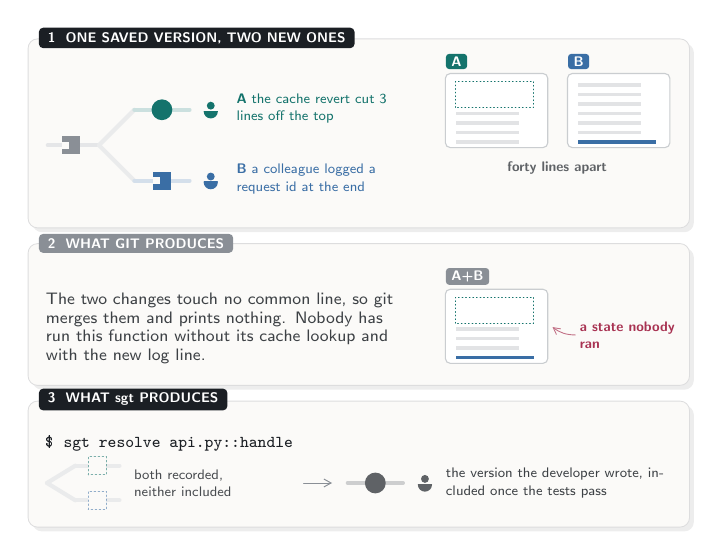
\begin{tikzpicture}[x=1mm, y=1mm, line cap=round, font=\sffamily]

% one function body. #1 x, #2 y of top edge, #3 mode: t / b / a
% t = the three lines at the top are gone.  b = a line added at the bottom.
\newcommand{\fbody}[3]{%
  \draw[card, color=sgtGrey!45, fill=white] (#1,{#2-9.4}) rectangle ({#1+13},#2);
  \foreach \yy in {-1.4,-2.6,-3.8,-5.0,-6.2,-7.4,-8.6}
    {\fill[sgtGrey!25] ({#1+1.3},{#2+\yy-0.3}) rectangle ({#1+9.4},{#2+\yy+0.15});}
  \if#3b\else
    \fill[white] ({#1+0.9},{#2-4.4}) rectangle ({#1+12.1},{#2-0.9});
    \draw[fCache, line width=0.3pt, densely dotted]
      ({#1+1.3},{#2-4.3}) rectangle ({#1+11.2},{#2-1.0});
  \fi
  \if#3t\else
    \fill[fIdx] ({#1+1.3},{#2-8.9}) rectangle ({#1+11.2},{#2-8.45});
  \fi}
% #1 x, #2 y of body top, #3 colour, #4 letter
\newcommand{\fbodytag}[4]{%
  \node[tag, fill=#3, text=white, anchor=south west,
        font=\sffamily\bfseries\fontsize{5.0}{5.8}\selectfont] at (#1,{#2+0.5}) {#4};}

% ============== 1: where the two versions come from ==================
\panel{0}{38}{84}{24}{sgtInk}{1\ \ ONE SAVED VERSION, TWO NEW ONES}

\draw[rail=sgtGrey] (2.5,48.5) -- (9.0,48.5);
\opext{5.5}{48.5}{sgtGrey}
\draw[raildim] (9.0,48.5) -- (13.5,53.0);
\draw[raildim] (9.0,48.5) -- (13.5,44.0);
\draw[rail=fCache] (13.5,53.0) -- (20.5,53.0); \oprew{17.0}{53.0}{fCache}
\draw[rail=fIdx]   (13.5,44.0) -- (20.5,44.0); \opext{17.0}{44.0}{fIdx}
\whodev{23.2}{53.0}{fCache}
\whodev{23.2}{44.0}{fIdx}

\node[anchor=west, text width=21mm, align=left, inner sep=0, text=fCache,
      font=\sffamily\fontsize{5.4}{6.2}\selectfont] at (26.4,53.2)
  {\textbf{A} the cache revert cut 3 lines off the top};
\node[anchor=west, text width=21mm, align=left, inner sep=0, text=fIdx,
      font=\sffamily\fontsize{5.4}{6.2}\selectfont] at (26.4,44.2)
  {\textbf{B} a colleague logged a request id at the end};

\fbody{53.0}{57.6}{t}\fbodytag{53.0}{57.6}{fCache}{A}
\fbody{68.5}{57.6}{b}\fbodytag{68.5}{57.6}{fIdx}{B}
\node[acc=sgtInk!70, anchor=north] at (67.2,46.8) {forty lines apart};

% ===================== 2: what git produces ==========================
\panel{0}{18}{84}{18}{sgtGrey}{2\ \ WHAT GIT PRODUCES}

\node[anchor=north west, text width=46mm, align=left, inner sep=0, text=sgtInk!85,
      font=\sffamily\fontsize{5.7}{6.7}\selectfont] at (2.2,29.8)
  {The two changes touch no common line, so git merges them and prints nothing.
   Nobody has run this function without its cache lookup and with the new log
   line.};

\fbody{53.0}{30.2}{a}
\fbodytag{53.0}{30.2}{sgtGrey}{A+B}
\annot{69.5}{24.4}{66.6}{25.4}{18}{fExport}
\node[anchor=west, text width=13mm, align=left, inner sep=0, text=fExport,
      font=\sffamily\bfseries\fontsize{5.4}{6.2}\selectfont] at (70.0,24.4)
  {a state nobody ran};

% ===================== 3: what sgt produces ==========================
\panel{0}{0}{84}{16}{sgtInk}{3\ \ WHAT \textsf{sgt} PRODUCES}

\node[anchor=north west, inner sep=0, text=sgtInk,
      font=\ttfamily\fontsize{5.6}{6.4}\selectfont] at (2.2,11.6)
  {\$ sgt resolve api.py::handle};

\draw[raildim] (2.4,5.6) -- (6.0,7.8);
\draw[raildim] (2.4,5.6) -- (6.0,3.4);
\draw[raildim] (6.0,7.8) -- (11.6,7.8); \opghost{8.8}{7.8}{fCache}
\draw[raildim] (6.0,3.4) -- (11.6,3.4); \opghost{8.8}{3.4}{fIdx}
\node[anchor=west, text width=20mm, align=left, inner sep=0, text=sgtInk!80,
      font=\sffamily\fontsize{5.4}{6.2}\selectfont] at (13.4,5.6)
  {both recorded,\\neither included};

\draw[-{Straight Barb[length=0.9mm,width=1.0mm]}, line width=0.35pt, color=sgtGrey]
  (35.0,5.6) -- (38.6,5.6);
\draw[rail=sgtInk] (40.6,5.6) -- (47.6,5.6); \oprew{44.1}{5.6}{sgtInk!70}
\whodev{50.4}{5.6}{sgtInk!70}
\node[anchor=west, text width=29mm, align=left, inner sep=0, text=sgtInk!85,
      font=\sffamily\fontsize{5.4}{6.2}\selectfont] at (53.0,5.6)
  {the version the developer wrote, included once the tests pass};

\end{tikzpicture}

  \Description{\FigForkDescription}
  \caption{\FigForkCaption}
  \label{fig:fork}
\end{figure}

When two edits change the same function from the same starting version, \sgt{}
records both, includes neither, and asks the developer. This is the commitment that
costs the most goodwill in the first week, so we want to be precise about whose
behaviour we are departing from and why theirs is right.

Git merges text and knows nothing about what a function is. A system that has
to work on every text file in every language anyone will ever write can afford to
know nothing else, which is why \cmd{git merge} is useful on a Makefile. In the case
Figure~\ref{fig:fork} draws, two people had last saved the same version of
\sym{api.py::handle}, one of them reverted a caching feature, which took the cache
lookup out of the first three lines, and the other added a request identifier to the
logging block forty lines away, with no line in common. Git merges the two without
comment, and the function that comes out has never been run in that state by
anybody. \sgt{} sees one function with two versions from one parent, names it, and
stops. \cmd{sgt resolve api.py::handle} prints the two versions beside each other
and asks \cmd{pick [l]eft / [r]ight / [e]dit / [q]uit}, where the third choice opens
the file in the developer's editor and the fourth leaves the fork open, and whatever
they write has to pass the project's test command before \sgt{} will include it.
Where no test command is configured the developer supplies the verdict with
\cmd{--override pass} and a \cmd{--reason}, and the reason and their name are
recorded beside the resolution, so the next person to read that function finds out
why it looks the way it does.

A developer pays for this by being stopped in cases where the merge would have been
fine, and in one of those cases \sgt{} stops for nothing at all, since deleting a
function and adding it back with byte-identical content in two places produces two
versions from one parent and \sgt{} treats content that agrees exactly as a
disagreement. The design is a fail-stop commitment in Schlichting and Schneider's
sense~\cite{schlichting1983}: the system converts a potentially-wrong state (a
textual merge whose correctness nobody has verified) into a detectable halt (the
developer is asked). Fail-stop costs availability---the tool is unavailable until the
developer answers---in exchange for a guarantee about everything it does let through:
if the system did not stop, the included version is one a person chose, not one a
program composed. The read layer inherits this property: every attribution,
dependency display, and consequence preview rests on versions that entered through a
human decision, so the reports are as trustworthy as the decisions they trace back to.
A silent textual merge would break that chain, because the function it produces has
never been chosen by anybody, and the next revert that touches it would be operating on
text whose provenance is a program's guess rather than a person's act.

We hold the commitment loosely, because a
developer who merges thirty branches a day would reasonably weigh the two the other
way, and for them the current design is worse. The 18$\times$ amplification
Section~\ref{sec:session-rate} reports is the measured cost of choosing correctness
over availability at this grain, and a tool builder facing the same choice should
treat that number as a lower bound on what fail-stop costs at the function level.

The deeper reason for accepting that cost is the context in which the tool
operates. A developer who typed the competing versions themselves would have read
both, would hold a model of what each does, and could evaluate a textual merge in
seconds. A developer whose agent produced one version while a colleague's agent
produced the other has read neither, holds no model of the interaction between them,
and would accept a textual merge not because they verified it but because the tool
offered no reason to look. Shen and Tamkin measured this directly: developers who
relied on AI assistance scored 17\% lower on assessments of the code they had just
produced, with debugging---recognising when code is wrong---showing the largest
gap~\cite{shen2026skills}. The fork rule is designed for the developer in that
degraded state: it forces a decision point that requires looking at the two versions,
which is the cognitive engagement their earlier delegation removed. A tool that
silently merges code its user has not read, in a context where the user's capacity to
read critically has already declined, is compounding the problem it was built to
address.

\subsection{The names are inferred, and correcting one moves labels only}
\label{sec:names}

Every figure in this paper labels a group of edits with a name like
\emph{price cache}, and those names are the part of \sgt{} that guesses. Functions
that changed in the same saves and that refer to one another are grouped together,
using the change coupling signal established by Zimmermann et al.\ and Ying et
al.~\cite{zimmermann2004,ying2004} and a community detection method over the
resulting graph~\cite{traag2019}. The reason a graph algorithm finds real features
rather than arbitrary cuts is that codebases exhibit what Simon called
\emph{near-decomposability}: interactions within a subsystem are strong and frequent
while interactions between subsystems are weak and
infrequent~\cite{simon1962}. Community detection recovers that structure because
it was designed to, and the known exception---a hub function called from
everywhere---is the same entity that breaks feature location in the literature and
that Section~\ref{sec:discussion-synthesis} reports as the main source of
grouping errors here: it pulls otherwise separate requests into one community
because the coupling signal cannot tell structural proximity from shared purpose.

A language model then reads the saves in a group
and writes the label, which is the descendant of a task attempted before language
models existed, when Buse and Weimer generated a description of a change out of the
change itself~\cite{buse2010}. The label draws from the developer's words rather than
from the code's identifier names. Nguyen and
Glassman showed that the naming a model uses in its output and the naming a
developer uses to describe the same behaviour systematically
mismatch~\cite{nguyen2024}. A label derived from identifier names would therefore speak the
model's language rather than the developer's, and the developer who later searches
for ``the caching'' would find nothing under whatever the model called its cache
class. Membership is computed from the code and the label is written from the words,
and those two steps fail in different ways, so we treat them separately. The
grouping is also systematically finer than the request: a community detection
algorithm cuts where the coupling is weak, not where the developer stopped
typing, so one request that touches several disjoint parts of the code becomes
several features. Section~\ref{sec:discussion-synthesis} reports a median of
4--6 features per request across four repositories. The result is a sub-intent
decomposition rather than an intent recovery---the developer gets a vocabulary
for the structural neighbourhoods their request produced, not a map back to what
they asked for. The finer grain has a cost and a benefit. The cost is that the
developer cannot name what they asked for in one selection; they must merge or
select several. The benefit is that operations work at a finer level than the
request: the developer who asked for caching and later wants only the TTL
helper removed can name that piece without reverting the whole request. The
mismatch is in level as well as in number: the
developer thinks at the level of ``the price cache'' (one purpose, one name) while
the tool presents four structural communities inside it, a difference
Section~\ref{sec:discussion-synthesis} traces to Rosch's distinction between
basic-level and subordinate categories~\cite{rosch1978}.

We chose to operate at the subordinate level rather than the basic level for a
reason that becomes clear only when the developer acts on the grouping. A
request boundary is unstable: it depends on what the developer typed, which changes
between ``implement caching'' (one request) and ``add a TTL helper, then wire it
into the handler'' (two requests for the same code). A structural boundary is
stable: it depends on which functions call which others, which does not change when
the developer rephrases. A revert, a restore, or a dependency warning all need a
boundary that means the same thing regardless of when the developer asks---and a
boundary defined by coupling has that property while a boundary defined by request
phrasing does not. The over-decomposition is therefore not an error in the
clustering but a consequence of choosing stability over correspondence: the tool
gives four addressable pieces where the developer expected one, because those four
pieces are the ones whose membership will not shift when the next request arrives.
The cost (merging to act at the request level) is paid once; the benefit (stable
addresses for operations) pays on every subsequent use.

We considered asking the developer to confirm the grouping at save time and decided
against it, because answering that question takes the same knowledge commit hygiene
takes, and a developer who could reliably answer it could also have staged the
hunks. Shipman and Marshall showed that systems which ask users to formalise their
own work get abandoned~\cite{shipman1999}; the design they arrived at has the system
propose a structure the user may accept, modify, reject, or leave alone, which is
the arrangement here. Our conditions are easier than theirs: the structure their
systems tried to elicit was tacit, so a user had first to work out what they thought.
The structure \sgt{} recovers was spoken in a request before any of the code
existed---though not at the grain the tool produces, since one request typically
splits into several structural clusters. The reason it needs recovering at all
is that nothing wrote it down. What matters is therefore not whether the guess is
right but what a wrong one costs, and correcting one moves labels and touches no
recorded edit. \cmd{sgt feature rename 001f73c2 "price cache"} renames a group whose
identifier stays what it was, \cmd{sgt feature regroup} moves functions between
groups, and \cmd{sgt save --as "price cache"} files a new save into a group that
already exists. Because identifiers survive all three, a revert written down in a
code review comment last month still removes the same edits after somebody renames
the group today.

The deeper function of inferred names is coordination. Clark's analysis of language
use shows that people who need to refer to the same thing build a shared
vocabulary through proposal and acceptance: one party offers a term, the other
either adopts it or repairs it, and after a few exchanges the term is common
ground~\cite{clark1996}. A version control system that infers feature names is
proposing one half of that exchange---offering ``price cache'' as the term both the
developer and the tool will use to pick out a set of edits. If the developer types
\cmd{sgt revert "price cache"} the proposal has been accepted and the name is
grounded; if they rename it, the repair has completed the same grounding through a
different path. Either way, the tool and developer now share a vocabulary for the
codebase, and that vocabulary enters the developer's prompts to the AI assistant,
which is why the ``prompt specificity'' measure in Section~\ref{sec:findings-process}
tests whether the tool's names reached the developer's language. A wrong label costs
a rename (one command, no data moved); a missing shared vocabulary costs every
subsequent conversation about the code, because the developer and the tool have no
common referent for the set of edits they both need to name.

Two failures show up often enough that a reader will hit them. A function that
everything calls, an argument parser or a logging helper, changes in nearly every
save and pulls otherwise unrelated work into one group, and the fix is a regroup the
developer has to notice they need. A save with no message gives the language model
less to read, and \sgt{} says so at the time, printing \cmd{\textperiodcentered{} no words captured}
under the save it just wrote, because the label summarises what the developer said
about the work and a developer who says nothing gets a name derived from the code
alone.

\subsection{What \sgt{} will not do}

\sgt{} writes no code of its own. Every byte in the working files came from the
developer or their agent, apart from the three-way merge splice in
Section~\ref{sec:sets}, which reports every case it cannot perform cleanly. We have
been asked more than once during this work why \sgt{} does not hand the shared
function to a language model and have it redrafted after a revert. We considered it
seriously and rejected it for one reason: a revert whose output depends on a
model's judgement produces a file whose correctness the developer can verify only
by reading every line the model touched, which is the labour Section~\ref{sec:scenarios}
argued this tool should eliminate. A revert whose output is computed from the
records the developer already validated produces a file whose correctness follows
from the records, and the developer's test suite decides whether the composition
is sound. The cost is that a subtraction which overlaps later work requires a hand
edit; the benefit is that the developer knows what they are reading. Bansal et
al.\ found that AI explanations increase acceptance whether or not the underlying
recommendation is correct~\cite{bansal2021}; a model-in-the-loop revert would
face the same problem, because the developer would have to judge whether the
model's redrafted function is correct, and the tool's report that it passed tests
is exactly the kind of explanation that increases acceptance without increasing
accuracy. The refusal has a deeper justification. A version control system is
infrastructure: it sits beneath every other decision, and a revert that is wrong
invalidates every test, every review, and every deployment that followed it. An
AI assistant is a collaborator: its suggestions are proposals that a developer
accepts, modifies, or rejects one at a time, and a wrong suggestion costs one
undo. The failure modes are not symmetric. A wrong line completion costs the
developer a delete; a wrong revert costs them their codebase state, and the
difference in blast radius is the difference between a tool that should reach for
a model (the assistant) and one that should not (the substrate). The trend toward
model-in-the-loop for every operation conflates the two roles, and the
conflation is invisible as long as the model is correct. The moment it is wrong,
the developer discovers that the substrate contained a guess they never verified,
and the cost of discovering it late is what Section~\ref{sec:discussion}
measures.

\sgt{} also does not stand between a developer and git. The records are files under
\cmd{.sgt/} committed alongside the code, \cmd{sgt git <args>} passes through to git
untouched, a colleague who has never installed \sgt{} clones an ordinary repository
with an ordinary history, and there is no server and no background process. Two
commands refuse to run: \cmd{switch} stops when there are unsaved edits, because
\sgt{} has nowhere to put them, and names the files and prints \cmd{record them with
`sgt save', or commit / `git restore' those files, then re-run}; \cmd{restore} stops
when putting a set back would leave two versions of one function live, and there its
message names the edits by identifier while the function whose two versions caused
the refusal goes unnamed, which is the rough edge Section~\ref{sec:walkthrough}
reports us fixing in the fork warning and not here. Everything else
\sgt{} finds wrong it reports, and then it proceeds.

\subsection{From the five operations to the commands a developer types}

\begin{figure*}[t]
  \centering
  % Every operation sgt offers, grouped by what it does to the recorded set, with
% the state before and after each command and what each one costs.
% Prints as Figure 5, after the fork figure in Section 4.3.
\newcommand{\FigFourCaption}{The nine operations that act on the record, grouped
by what each one does to it. One command writes records and the other eight read
them or change which of them a version includes, and no argument anywhere in the
figure is a hash or a line number: every one of them is a request the developer
named, a branch, or a function.}

\newcommand{\FigFourDescription}{Three panels, one per group of operations. The
first panel holds the single operation that writes records, the second holds the
three that only read them, and the third holds the five that change which
records a version includes. Each row carries a small diagram of the set before
and after the command, the command itself, one sentence saying what the developer
gets, and one sentence in a grey band on the right saying what the operation
costs. Each diagram draws one horizontal line per request with a mark for every
edit filed under that request, as in Figure 1, and a dotted outline is an edit
the version no longer includes.}

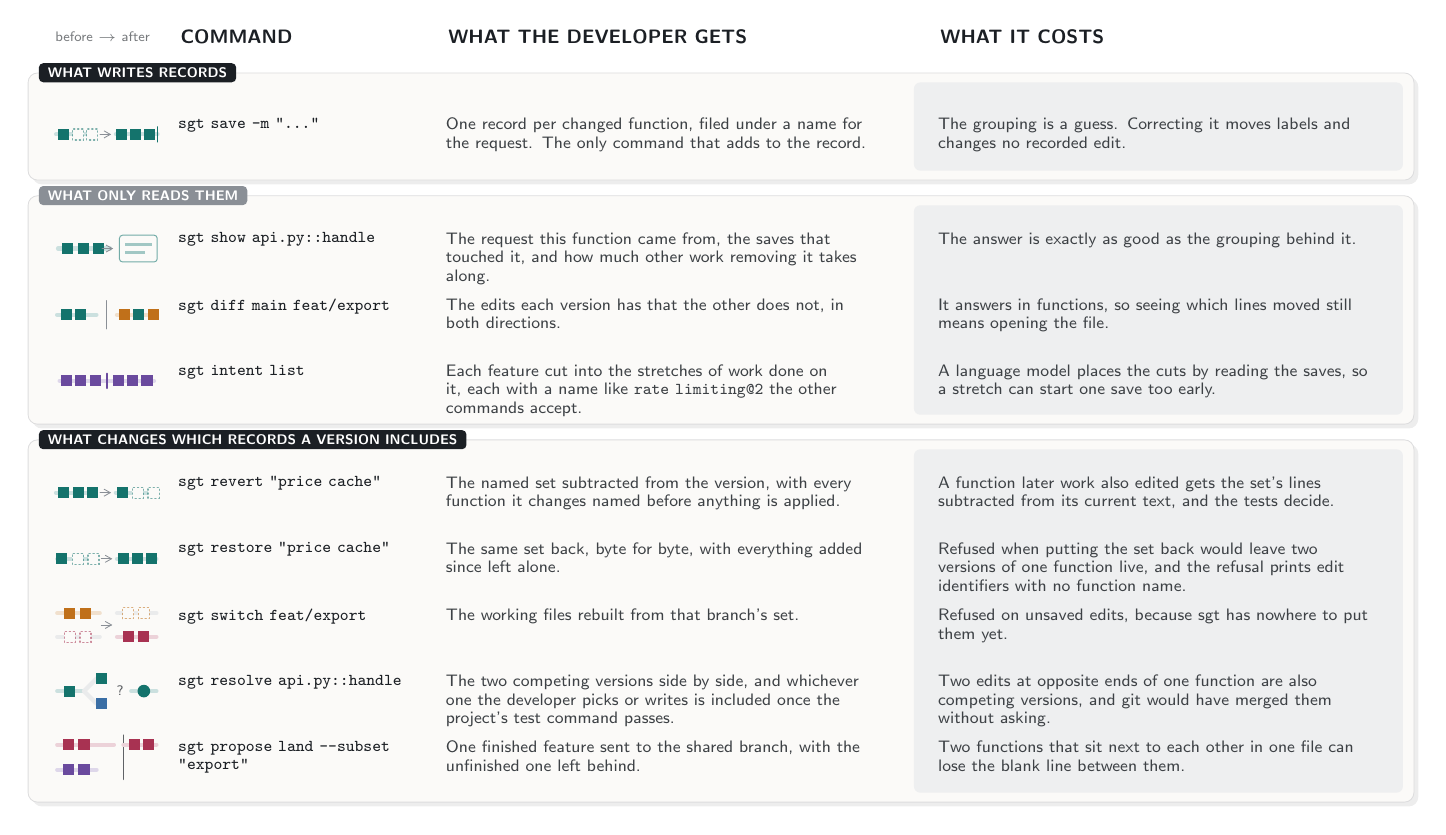
\begin{tikzpicture}[x=1mm, y=1mm, line cap=round, font=\sffamily]
% narrow ragged columns, so break a line early rather than hyphenate a word
\hyphenpenalty=10000 \exhyphenpenalty=10000

% the thumbnails carry the before/after convention, so the column says so itself
\node[anchor=west, inner sep=0, text=sgtInk!60,
      font=\sffamily\fontsize{5.0}{5.8}\selectfont] at (3.4,104.6)
  {before \ttarrow{} after};
\node[hd, anchor=west] at (19,104.6)    {COMMAND};
\node[hd, anchor=west] at (53,104.6)    {WHAT THE DEVELOPER GETS};
\node[hd, anchor=west] at (115.5,104.6) {WHAT IT COSTS};

% one group of operations. The cost column gets a band of its own on the right,
% the same band Figure 2 uses, so the reader can read that column straight down.
% #1 y, #2 height, #3 tab colour, #4 tab text
\newcommand{\opgroup}[4]{%
  \panel{0}{#1}{176}{#2}{#3}{#4}
  \fill[wGrey, rounded corners=0.8mm] (112.5,{#1+1.2}) rectangle (174.6,{#1+#2-1.2});}

% #1 y of the first text line, #2 thumbnail, #3 command, #4 gets, #5 costs
\newcommand{\oprow}[5]{%
  \node[inner sep=0] at (10,{#1-2.1}) {#2};
  \node[anchor=north west, text width=32mm, align=left, inner sep=0, text=sgtInk,
        font=\ttfamily\fontsize{5.6}{6.6}\selectfont] at (19,#1) {#3};
  \node[anchor=north west, text width=55mm, align=left, inner sep=0, text=sgtInk!85,
        font=\sffamily\fontsize{5.7}{6.7}\selectfont] at (53,#1) {#4};
  \node[anchor=north west, text width=56mm, align=left, inner sep=0, text=sgtInk!85,
        font=\sffamily\fontsize{5.7}{6.7}\selectfont] at (115.5,#1) {#5};}

% =================== what writes records ==================================
% One row, and the group holding one row is the point: the developer types one
% command to add to the record, and everything else in the figure decides what
% that record is read for or what a version does with it.
\opgroup{86.4}{13.6}{sgtInk}{WHAT WRITES RECORDS}

% Centred in its panel rather than hung from the top of it, so that the space
% around the one row reads as emphasis and not as a row somebody took out.
\oprow{94.3}{\thsave}{sgt save -m "..."}
  {One record per changed function, filed under a name for the request. The only
   command that adds to the record.}
  {The grouping is a guess. Correcting it moves labels and changes no recorded
   edit.}

% =================== what only reads them =================================
\opgroup{55.4}{29}{sgtGrey}{WHAT ONLY READS THEM}

\oprow{79.8}{\thwhy}{sgt show api.py::handle}
  {The request this function came from, the saves that touched it, and how much
   other work removing it takes along.}
  {The answer is exactly as good as the grouping behind it.}
\oprow{71.4}{\thdiff}{sgt diff main feat/export}
  {The edits each version has that the other does not, in both directions.}
  {It answers in functions, so seeing which lines moved still means opening the
   file.}
\oprow{63.0}{\thckpt}{sgt intent list}
  {Each feature cut into the stretches of work done on it, each with a name like
   {\ttfamily rate limiting@2} the other commands accept.}
  {A language model places the cuts by reading the saves, so a stretch can start
   one save too early.}

% ============ what changes which records a version includes ===============
\opgroup{7.4}{46}{sgtInk}{WHAT CHANGES WHICH RECORDS A VERSION INCLUDES}

\oprow{48.8}{\threvert}{sgt revert "price cache"}
  {The named set subtracted from the version, with every function it changes
   named before anything is applied.}
  {A function later work also edited gets the set's lines subtracted from its
   current text, and the tests decide.}
\oprow{40.4}{\threstore}{sgt restore "price cache"}
  {The same set back, byte for byte, with everything added since left alone.}
  {Refused when putting the set back would leave two versions of one function
   live, and the refusal prints edit identifiers with no function name.}
\oprow{32.0}{\thswitch}{sgt switch feat/export}
  {The working files rebuilt from that branch's set.}
  {Refused on unsaved edits, because \sgt{} has nowhere to put them yet.}
\oprow{23.6}{\thfork}{sgt resolve api.py::handle}
  {The two competing versions side by side, and whichever one the developer
   picks or writes is included once the project's test command passes.}
  {Two edits at opposite ends of one function are also competing versions, and
   git would have merged them without asking.}
\oprow{15.2}{\thsubset}{sgt propose land --subset "export"}
  {One finished feature sent to the shared branch, with the unfinished one left
   behind.}
  {Two functions that sit next to each other in one file can lose the blank line
   between them.}

\end{tikzpicture}

  \Description{\FigFourDescription}
  \caption{\FigFourCaption}
  \label{fig:operations}
\end{figure*}

Figure~\ref{fig:operations} sets out the nine operations that act on the record,
each with its cost beside it, and the five operations Section~\ref{sec:scenarios}
ended on are four commands and one thing that needs no command. Recording a
boundary without declaring it is
\cmd{sgt save -m}, run whenever the developer feels like running it, since the
grouping is recovered afterwards from the code. Seeing the work one request produced
is \cmd{sgt show "rate limiting"}, or \cmd{sgt show "rate limiting@1"} for one
stretch of work on it alone. Removing a named set is
\cmd{sgt revert "price cache"}, and carrying one to another branch is
\cmd{sgt propose land --subset "export"}, which declines a subset that omits a group
another chosen group depends on and names the group that is missing. Each of those
four takes as its argument a phrase somebody used while the work was happening, so
the manual recovery Section~\ref{sec:scenarios} described is replaced by a named
command---on repositories where the store reproduces the committed bytes. Where
it does not (27 of 28 outside repositories), the command refuses rather than
producing a wrong file, and the developer is back to the manual recovery with no
help from the tool (Section~\ref{sec:session-rate}).

Discovering the
layering needs no command at all wherever the references resolved, because the cache
edits record that they were built on \sym{api.py::\_bucket} and therefore on the rate
limiter, so the developer has at any later moment the fact they needed at 14:30 and
did not have. Where they did not resolve, the layering is simply absent rather than wrong, and the
developer is back to reading the code, which is the position the ambiguity rule
above trades down to on purpose. On 35 corpus repositories, 93\% of ops carry no
reference at all, because resolution requires a globally unique function name---so
the absence is the common case, not a rare failure. The 7\% that do resolve tend to
be cross-module calls (a handler calling a cache function in another file, a test
importing a fixture), which are precisely the dependencies whose absence would break
the code silently---so the coverage is thin but concentrated on the cases where a
human would not have noticed the dependency either. Where resolution is absent, the
developer's test suite is the only oracle, and \sgt{} says so in the revert output
(``still references removed code'') only when it can, which on most repositories is
never. The implication for adoption is blunt: a developer whose repository has few
cross-module calls will never see a dependency warning, and will discover that the
tool offers no protection there only when a revert breaks something silently.

A reader should treat the dependency display as a bonus that fires
occasionally rather than a guarantee the design rests on; the design rests on set
arithmetic over edits, and the dependency enriches a revert without being required
for one. The rest of
what a developer types is housekeeping around those nine, \cmd{sgt init} to begin,
\cmd{sgt log} and \cmd{sgt sync} to see where things stand, and the
\cmd{sgt feature rename} of Section~\ref{sec:names} to correct a name, none of which
changes which edits a version includes. Section~\ref{sec:walkthrough} runs these in
order on one repository.

\section{One Repository, Five Sittings}
\label{sec:walkthrough}

The repository here is a five thousand line Python service that answers price
quotes for a trading dashboard, and the first sitting is the hour
Figure~\ref{fig:two-records} draws. We assembled the sequence from sessions we ran
while building \sgt{} so that one repository contains the five operations
Section~\ref{sec:scenarios} asked for, in that order, followed by the one case
where \sgt{} stops and asks. Every command below runs and every block of output
came out of \sgt{} as it is today. Output lines too wide for this column are
wrapped, at the \ttdot{} separators where a line offers a list of alternatives,
and are otherwise unchanged. Read the sequence for which decisions the
developer is asked to make, and when in the work they arrive.

\subsection{Monday, 14:02 to 15:20: two saves and four names}

The developer made three requests in that hour, and the agent renamed a function
on its own initiative. At 14:33, with the rate limiting finished and the price
cache first drafted, the developer saved.

\begin{out}
\$ sgt save -m "rate limiting and a price cache on quotes"\\
\ttok{} save c39ab2f "rate limiting and a price cache on quotes"\\
~~\ttbranch{}\ttnew{} new feature (4a1c9e02) \ttdash{} unnamed; name it:\\
~~\ttvert{}~~~~sgt feature rename 4a1c9e02 "<label>"\\
~~\ttvert{}~~~~api.py::\_bucket, api.py::\_key, api.py::\_window +1 more\\
~~\ttbranch{}\ttnew{} new feature (001f73c2) \ttdash{} unnamed; name it: \dots\\
~~\ttvert{}~~~~cache.py::get\_cached, cache.py::\_ttl, db.py::query +1 more\\
~~\ttlast{}\ttnew{} new feature (9d20b18a) \ttdash{} unnamed; name it: \dots\\
~~~~~~~db.py::fetch\_row, api.py::export\_row, util.py::load\_row +1 more\\
~~\ttwarn{} one save touched 3 features \ttdash{} deliberate? `sgt log --map'\\
~~~~~shows them; `sgt feature regroup move' re-files work\\
~~\ttundo{} reverse this save:~~sgt undo
\end{out}

\noindent
The developer typed one sentence and \sgt{} wrote twelve records. The three groups
have no names yet, because \sgt{} writes records when the developer saves and works
out the names when the developer next reads, and a name costs a language model call
that has no business running while somebody is mid-session. The warning is the one
line here that resembles what git asks for, and \sgt{} printed it after the save was
already written. The developer read it, agreed the sitting had been mixed, and
carried on, and Section~\ref{sec:scenarios} opened with exactly that case.

The second save at 15:20 covered the retry policy and a rework of the cache the
agent made while adding the retry. By then the first save's groups had names, so its echo listed
\cmd{\ttdisc{} Price Cache (001f73c2)} for the group that already existed and
\cmd{\ttnew{} new feature (7c02b4d1)} for the retry work.
\cmd{sgt log --tree} afterwards printed the four groups the hour produced.

\begin{out}
Rate Limiting (4a1c9e02) \ttdot{} 4 symbol(s)\\
Price Cache (001f73c2) \ttdot{} 4 symbol(s)\\
Retry Policy (7c02b4d1) \ttdot{} 3 symbol(s)\\
Row Accessors (9d20b18a) \ttdot{} 5 symbol(s)
\end{out}

\noindent
Three of the four names are what the developer would have written. The fourth is
the agent's unrequested rename, named from the code because the developer never
said anything about that part of the work, the failure
Section~\ref{sec:names} predicts. It is also the only one of the four whose name
nobody needs, so nobody corrected it.

\subsection{Thursday: changing the rate limiter}

The fixed one minute window has to become a sliding one, and the developer starts
from what the rate limiting is now.

\begin{out}
\$ sgt show "Rate Limiting"\\
feature 4a1c9e02~~"Rate Limiting"\\
~~4 edits \ttdot{} 4 symbols in 1 file \ttdot{} last touched 3d ago\\
~~symbols~~~~~~api.py::\_bucket, api.py::\_key, api.py::\_window,\\
~~~~~~~~~~~~~~api.py::handle\\
~~saves~~~~~~~~c39ab2f~~rate limiting and a price cache on quotes\\
~~reverting this removes 4 edits
\end{out}

\noindent
The four functions are the answer to the question that took four runs of
\cmd{git log -L} in Section~\ref{sec:scenarios}, and nothing here required the
developer to guess that four was the right number of places to look. What this
output does not say is that the price cache calls \sym{api.py::\_bucket} and
therefore sits on top of the rate limiter, so a sliding window is a change
underneath work that already depends on it. The record holds that fact, because
the cache's edits name the functions they refer to, and \cmd{show} does not print
it. The developer finds it out on Wednesday instead, when \cmd{propose land}
refuses a subset for that reason, and a \cmd{show} that printed it here would
have cost us one line.

The agent rewrites \sym{api.py::\_window} and \sym{api.py::\_bucket} and leaves the
other two functions alone, and the developer saves, naming the group this time
because they already know which one it is.

\begin{out}
\$ sgt save --as "Rate Limiting" -m "sliding window, 60s of buckets"\\
\ttok{} save 1f0aee3 "sliding window, 60s of buckets"\\
~~\ttlast{}\ttdisc{} Rate Limiting (4a1c9e02)~~api.py::\_bucket, api.py::\_window\\
~~\ttok{} named "Rate Limiting"
\end{out}

\noindent
\cmd{--as} is the one place a developer states a grouping by hand, and it changed
nothing here, because both functions were already in that group and the edits would
have been filed there without it. They typed it because they knew the answer and
had no reason to let \sgt{} work it out. The rate limiting now has two stretches of
work on it, and \cmd{sgt log --focus 4a1c9e02} names both.

\begin{out}
\ttdisc{} Rate Limiting~~4a1c9e02~~\ttdot{}~~2 checkpoint(s)\\[0.35ex]
~~~[0\ttfull\ttfull\ttfull]~~4a1c9e02@0~~:rate-limiting~~Rate Limiting\\
~~~[1\ttfull\ttfull\ttempty]~~4a1c9e02@1~~:sliding-window~~Sliding Window\\[0.35ex]
~operate:\\
~~~~sgt revert 4a1c9e02:sliding-window~~(one checkpoint, by name)\\
~~~~sgt revert 4a1c9e02~~(whole feature)\\
~~~~sgt revert 4a1c9e02@1~~(by index)
\end{out}

\noindent
The developer never asked for these two stretches. \sgt{} cut the work where their
words changed, which in this repository is where one request ended and the next
began, and either half is addressable on its own, so
\cmd{sgt revert "Rate Limiting:sliding-window"} takes Thursday's work off and
leaves Monday's four edits in place. The bar beside each name puts that
checkpoint's edits in their place in the history, read left to right, with a middle
dot where a span of the history holds none of them, so the terminal spends four
characters on the encoding Figure~\ref{fig:two-records} spends a panel on. The last three lines exist because we watched
people on our own team discover that a stretch of work had a name and then stop,
not knowing which command would accept it.

\subsection{The following Monday: taking the cache out}

The cache serves a stale price for up to sixty seconds and has to go.

\begin{out}
\$ sgt revert "Price Cache"\\
~~~~[the log region redrawn, with the 6 removed edits marked]\\
~~subtracted from shared code (later work kept): api.py::handle\\
~~removed going forward: cache.py::get\_cached, cache.py::\_ttl,\\
~~~~~db.py::query\\
~~\ttwarn{} still references removed code (fix or revert separately):\\
~~~~~api.py::export\_row, util.py::load\_row, util.py::save\_row\\[0.35ex]
apply this revert? [y/N]
\end{out}

\noindent
The retry policy edited \sym{api.py::handle} after the cache had edited it, so
that function keeps the retry work and loses the cache's three lines, and a
request made a week ago comes out from under a change made yesterday. Two
functions existed only for the cache and come out with it, which empties
\sym{cache.py} and removes the file, and
\sym{db.py::query} loses the parameter the cache added and goes back to the text it
had at 14:02. The three functions in the last line are row accessors the agent
rewrote during its rename, and it pointed all three at \sym{get\_cached} while it
was in there, so their edits belong to a request the developer is keeping and name
a function the revert deletes. \sgt{} names them and proceeds, because whether the
repair is deleting three call sites or reverting the rename as well is not a
question about the recorded edits.

The developer answered \cmd{y} and ran the test suite. It failed in the three
places the report named and nowhere else, and the repair was deleting the cache
lookup from each of them. \sgt{} builds every one of these operations as set
arithmetic so that a revert can be taken back exactly, and the developer tested
that claim before trusting it.

\begin{out}
\$ sgt restore "Price Cache"\\
~~\ttok{} restore applied \ttdash{} 0 edit(s) removed, 6 added.\\
~~~~(`sgt undo' reverses this.)
\end{out}

\noindent
Putting the cache back returned \sym{cache.py}, \sym{db.py::query}, and
\sym{api.py::handle} to the bytes they held before the revert, and it left the
three call site repairs the developer had made in between alone, because a restore
adds records to the set and rebuilds the files from the result without reapplying
a patch. They had wanted the cache gone, so they reverted it a second time, and
that run printed the same three consequence lines as the first.

\subsection{Wednesday: shipping the export fix alone}

A bulk export endpoint has to ship to the release branch today, and the branch it
sits on also carries the retry policy, which is half finished. The export code goes
into a new \sym{export.py} and applies the rate limit before streaming, so
\sym{export.py::write\_csv} calls \sym{api.py::\_bucket}. Nobody thought about that
call as a dependency while writing it.

\begin{out}
\$ sgt propose create --base release\\
\ttok{} proposal 3f9a2c81b04d (base release, +17 op(s), 4 feature(s))\\
\$ sgt propose land 3f9a2c81b04d --subset "Quote Export"\\
\textnormal{$\times$} 'Quote Export' requires Rate Limiting -- include it in\\
~~--subset too
\end{out}

\noindent
The developer asked to move one group and \sgt{} named the group that has to come
with it, the fourth operation Section~\ref{sec:scenarios} asked for. The record of the call to \sym{api.py::\_bucket} was
written at the moment the export code was saved, and \sgt{} reads it now to answer
a question nobody was thinking about then. Git would have taken the cherry-pick and
the release branch would have failed to import.

\begin{out}
\$ sgt propose land 3f9a2c81b04d --subset "Rate Limiting" "Quote Export"\\
\ttok{} propose land release: 8b21c0d4e7fa (+8 op(s))
\end{out}

\noindent
Two groups went to the release branch in the order the records put them in, and the
half finished retry policy and the accessor rename stayed behind. Those two groups
are the stack from Section~\ref{sec:scenarios}, assembled without the branch that
had to exist before the work did.

\subsection{Thursday: two versions of one function}

A colleague on this repository had been editing \sym{api.py::handle} as well,
adding a request identifier to every outbound log line. The developer syncs.

\begin{out}
\$ sgt sync\\
\ttwarn{} sync origin/main: merged 4f2a1c8b93de\\
~~~~+7 op(s)\\
~~~~\ttwarn{} 1 OPEN FORK(S) \ttdash{} forked symbol(s) sit at the common\\
~~~~~~ancestor until resolved:\\
~~~~~~api.py::handle \ttarrow{} sgt resolve api.py::handle
\end{out}

\noindent
The remedy is printed as a function name because that is what the developer knows
about the situation. Underneath it there is a command that takes the two edge
identifiers directly, \cmd{sgt advanced merge-op 3c91ab02 8ee14d77}, and for the
first several months of this system's life that was the line the fork warning
printed, on the reasoning that it named the two things precisely. A developer who
reads it learns that two records are in conflict and still has to work out which
function they are in. Deriving the function's name and printing that instead is a
one-line change we made late, and it is the clearest instance in this repository of
a report that was accurate and useless. The two
versions of \sym{api.py::handle} are the one the cache revert produced, three lines
shorter at the top where the cache lookup had been, and the colleague's, one line
longer inside the logging block at the end. No line is common to the two changes,
so git merges them without comment, the case
Figure~\ref{fig:fork} draws. \sgt{} prints them beside each other and asks.

\begin{out}
\ttrule{} fork on api.py::handle \ttrule{}~~(\ttleft{} left = tip A~~\ttright{} right = tip B)\\
~~~~[the two versions of the function, side by side]\\
pick [l]eft / [r]ight / [e]dit / [q]uit:
\end{out}

\noindent
The developer picked \cmd{e}, merged the two by hand in about thirty seconds, and
\sgt{} ran the project's test command before including the result. We are not going
to claim the textual merge would have been wrong here. It would most likely have
been right, and \sgt{} charged thirty seconds and one interruption to establish
that. We designed for the case where the merge is wrong, one edit adding an early
return and the other edit's new code sitting below it, and the test run that would
have caught it happening on a branch nobody has pushed yet. A developer
who merges often and reads carefully is paying us for a certainty they already had.

\subsection{What this cost}

Across five sittings and one fork the developer made three decisions \sgt{} could
not make for them. They decided the export endpoint should ship without the retry
policy, they decided how the two versions of \sym{api.py::handle} should read, and
they decided that the three functions still calling the cache should lose that
call and keep the rest of the agent's rename. All three are decisions about the
code itself, and none of the three is a question about which lines belong in which
commit.

The developer paid for those three decisions in three places. One group of five
edits carries a name derived from the code, because nobody said anything about
that part of the work. The revert left \sym{api.py::handle} holding text nobody
had read, so their test suite decided whether the revert had worked. The fork
stopped them on a merge that was probably fine. The second and third of those are direct consequences of
Section~\ref{sec:sets} and Section~\ref{sec:fork}, and on a repository this size we
would choose both again. On a repository where twenty people edit the same
functions each day, the fork rule is the first thing we would expect to have to
change.

\section{What Would Show This Is Wrong}
\label{sec:study}

Three claims in this paper fail independently of one another, and each one fails
in a way that a different kind of evidence catches. The record either reproduces
the bytes the developer's editor and agent left in the files or it does not, and
that is a question about a program, settled by running it over histories that
already exist. The grouping either lines up with the requests a developer made or
it does not, and that is a question about an inference, settled by comparing it
against sessions where somebody happened to write the requests down. A developer
either gets more of these operations right with \sgt{} than without it, or does
not, and that is a question about people. The first has a procedure and a number we
can print today, the second is under way on a corpus we are still assembling, and
the third is designed and not yet run. Underneath all three, \sgt{} has been the
version control for its own repository since the day it first ran, which is where
every number in Section~\ref{sec:discussion} comes from and why the two prices
Section~\ref{sec:design} states most flatly are the two that cost us something
before they cost anybody else.

\smallskip\noindent\emph{Not one number in this section comes from that third
study.} The measure that decides the argument is not the time a task takes but the
errors a participant does not notice, and naming that before the data exists is the
only way to be believed about it afterwards.

\subsection{The rebuild has to be exact}
\label{sec:eval-exact}

If \sgt{} reassembles a file into bytes that differ from what the developer left
there, then every operation in Section~\ref{sec:design} is set arithmetic over a
fiction, and nothing else in this paper is worth reading. This is the one
measurement whose failure would end the work rather than qualify it, so it goes
first and it is the only one we insist on before adoption.

The procedure follows the shape of the claim. We walk a repository's history one
commit at a time, mine each commit into records, rebuild every file from the set of
records that commit's state implies, and compare the result against the blob git
holds, byte for byte. A repository passes at a commit only if every file matches, so a
single differing byte in a single file is a failure at that commit, and we will report
the fraction of files that rebuild rather than an average over repositories, because a
developer cares whether their file comes back and not whether most files do. The
corpus is open source Python and TypeScript repositories chosen for length of history
and nothing else, and we are still assembling it, so the only number this procedure has
produced comes from our own repository, which is the hardest case available to us
because records written by five different versions of our miner sit in it.

That number is fifty-six files that no valid set of records reproduces, one in seven of
the files whose records name functions, and Section~\ref{sec:unreproducible} gives that
denominator and says what is in the fifty-six. What we do not know is whether
fifty-six is the cost of our own format changes or the cost of the design, and since
five miner versions in fifty-seven days is a rate no adopter will ever match, the
corpus run is how we intend to separate the two: a repository \sgt{} has never touched
cannot have our migrations in it.

\subsection{Whether the grouping matches what was asked for}

The names in every figure in this paper are inferred, and a developer who types
\cmd{sgt revert "price cache"} is trusting that inference with the contents of
their files. The question is not whether the clustering scores well against a
partition somebody drew, which is how the untangling literature is evaluated for
the good reason that its authors had nothing better to compare against
(Section~\ref{sec:related}). The question is whether the set that comes back when
a developer names one request is the set of edits that request produced.

That question needs a corpus where the requests were recorded, which agent sessions
now supply as a matter of course, since the transcript of a session names each request
and the files the agent touched while carrying it out. We mine each repository without
reading any transcript, derive a reference grouping from the transcripts alone, and
then ask two things of every request in the session: how much of what that request
produced comes back when the developer names it, and how much else comes with it.
Those are the two ways a revert disappoints the person who ran it, the edit it missed
and left sitting in the file, and the edit belonging to a different request that it
carried off as well. They fail asymmetrically, and the second is worse, because a
developer who is handed too little notices when the code still runs the way it did and
a developer who is handed too much has already lost work they meant to keep.

We expect the shared helper to be where this measurement goes wrong, because
Section~\ref{sec:names} predicts it and fifty-seven days of daily use have not
stopped it happening. An argument parser or a logging function that changes in nearly every
save is coupled to everything by the signal the clustering reads, and it draws
otherwise unrelated requests into one group. If most of the disagreement between
our grouping and the transcripts turns out to sit on functions of that kind, then
the fix is to weight a function's coupling down as the number of things it couples
to grows, and that is a change to one term rather than to the design. If the
disagreement is spread evenly across ordinary functions instead, then the coupling
signal is not carrying the grouping and the developer should be asked at save
time, which is the design we argued against in Section~\ref{sec:names} and would
have to argue for.

\subsection{Three requests, a transcript, and code nobody in the room wrote}
\label{sec:eval-study}

\begin{table*}[t]
  \centering
  \caption{The six measures of the study in Section~\ref{sec:eval-study}, each
  with the result that would count against the design. The first row is the one we
  would report first, and the third row is the one a reader would expect us to
  report first.}
  \Description{A three-column table. The left column names six measures: undetected
  errors, correct submissions, time to completion, diff lines read, forks raised and
  judged pointless, and label corrections. The middle column states what the authors
  expect for each. The right column states, for each, the observation that would
  count against the design.}
  \label{tab:measures}
  \small
  \begin{tabular}{@{}p{0.235\textwidth}p{0.335\textwidth}p{0.355\textwidth}@{}}
    \toprule
    \textbf{What we measure} & \textbf{What we expect} &
      \textbf{What would count against us} \\
    \midrule
    Submissions the participant believed correct and that were not.
      & The gap here is wider than the gap in time. Removing a request touches
        code the participant never read, and in git nothing tells them so.
      & Equal rates in both conditions. The recovery we call expensive would then
        be something developers already do reliably, and Section~\ref{sec:scenarios}
        is a story about us. \\[0.6ex]
    Submissions that pass the check.
      & More of them with \sgt{}, and the ones that fail fail in the places
        \cmd{revert} named out loud.
      & A failure in \sgt{} that the preview did not name. A report that misses a
        consequence is worse than no report. \\[0.6ex]
    Time to the moment the participant says they are done.
      & Shorter with \sgt{}, and we would not publish this alone.
      & Shorter with \sgt{} while the first row is flat. \sgt{} would then be a
        convenience, and we have argued for it as something else. \\[0.6ex]
    Lines of diff the participant opened before submitting.
      & Far fewer with \sgt{}, since no command in
        Section~\ref{sec:design} asks anyone to look at a hunk.
      & Participants reading the diff anyway. They would be checking \sgt{}'s
        report rather than using it, and after twenty minutes of that they are
        doing the git task with extra steps. \\[0.6ex]
    Forks \sgt{} raised, and how many the participant judged pointless.
      & A small number, mostly judged pointless, all cheap.
      & Any participant switching the rule off, or a fork resolved by picking a
        side whose result then failed the check. Being stopped would have bought
        nothing. \\[0.6ex]
    Labels the participant corrected, and what the correction cost.
      & One or two renames, no regroups.
      & A regroup on the critical path of an operation. The inference would then
        be spending the developer's attention rather than saving it. \\
    \bottomrule
  \end{tabular}
\end{table*}

The study puts a developer in the position the paper is about, which means giving
them a repository whose code they did not write and the three sentences that
caused it. Each participant receives a five thousand line Python service, a
transcript of the session that produced its most recent hour of work, and three
tasks, each of which names one request from that transcript and asks for it to be
moved or removed without disturbing the other two. This is the
state of the developer in Section~\ref{sec:scenarios} a week later, and it is also
the state of the developer who picks up a colleague's branch on a Monday, and it
is the only arrangement we found in which every participant knows exactly as much
about the code as every other one. Participants who direct the agent themselves
each remember a different amount of what came back, and that remembering is the
thing whose absence we are claiming matters.

We recruit developers who use a coding agent as part of their ordinary work,
because the difficulty we describe belongs to them and to nobody else, and we ask
each of them to work through two repositories, one with git and one with \sgt{},
in a counterbalanced order. In the git condition they use whatever they normally
use, including a graphical client, since the argument is about what git's record
can express and not about anybody's command line fluency. Each repository holds
three requests whose edits interleave inside shared functions, and each has a
different set of three so that a participant who has learned the shape of the
first task cannot apply it to the second. The tasks are the three operations from
Section~\ref{sec:scenarios} with a checkable outcome: take one named request out
and leave the other two working, carry one request to a release branch on its own,
and find the earlier state of a request in order to change it. We leave the other
two scenarios out of the study because their outcome is a judgement about when to
commit and how to stack, and we would be scoring participants against our
preference rather than against a result.

A submission is correct when a script says so, and the script asks three
questions. The tests belonging to the removed request fail, the tests belonging to
the two kept requests pass, and no function outside the intended set differs from
the reference repository. That third question is the one that catches the failure
this paper is about, because a participant who removes the caching and quietly
takes half the retry policy with it has produced a repository that passes its own
tests.

The first row of Table~\ref{tab:measures} is the one that matters, because a
developer who spends an extra twenty minutes untangling a commit by hand has lost
twenty minutes, while a developer who submits a repository they believe is clean and
that still calls a function they deleted has lost something they will not find until
the release branch fails to import. Hand untangling fails silently, and a design whose
whole argument is that the developer no longer holds the decomposition has to be
measured against silent failure rather than against the clock. We collect time because
a reader would want it and because a tool that is correct and unbearably slow is not
adopted, and we would not publish a time difference as the finding.

The last two rows of Table~\ref{tab:measures} measure the prices we stated in
Section~\ref{sec:design} rather than the benefits, and they are there because a
study that measures only what a design buys is a study that cannot be wrong. A
fork stops the developer and a wrong label makes them type a rename, both of which
are countable inside the session, and both have a threshold past which we would
change the design rather than defend it.

\subsection{What none of this would tell us}

Only the first of the three claims can be pushed past by running more of the same,
since adding repositories to Section~\ref{sec:eval-exact} sharpens that number and
nothing else here improves with volume.

A recorded request is not an intention. A developer who types
\emph{make the price lookup faster} holds a view of what should change that the
sentence does not contain, and the agent's response is a guess at the remainder.
The alignment we measure against a transcript is therefore alignment with what was
said, and the transcript sets a ceiling on it that no better clustering can pass.
We think this is the right measurement anyway, on the ground that what was said is
what the developer will type when they come back to remove it, but a reader who
believes intention and utterance come apart more often than we do should read that
number as an upper bound on something smaller.

Two hours with a transcript is not a week of forgetting. The cost we describe in
Section~\ref{sec:scenarios} grows as a developer's memory of the session fades,
and our design substitutes reading somebody else's transcript for that fading.
A participant who has just read three sentences knows more about the session than
the developer who typed them a week ago, so the git condition in our study is
easier than the situation it stands for, and the difference we measure understates
the one that matters. We prefer the understatement to a study nobody can run.

Finally, every task in the study has an answer a script can check, and we chose
those three tasks for that reason. The operations a developer wants most may be
the ones with no checkable answer, and deciding whether a stack of two reviews
was the right shape is one of them. We can say what \sgt{} makes possible there
and we cannot measure it, and Section~\ref{sec:discussion} keeps that distinction.

\section{Pilot Study}
\label{sec:pilot}

We ran three pilots before the full study: one in each condition (sgt and git,
both on the same task set) and a third exercising the study apparatus end to end.
The first two were designed to find defects in the tool that would cost a real
participant their data point, and defects in the study design that would make a
result uninterpretable. The third tested the machinery between the participant's
machine and the facilitator's console---exactly the seam nobody had
exercised---and found a validity threat that neither task pilot could surface.
We report all three because the defects they found are consequences of design
commitments rather than accidents of implementation: a technical evaluation
establishes that a property holds across 10{,}237 operations; it takes a new
user to show that a property that holds still costs too much to use.

\subsection{What the pilots tested}

Six requests, drawn from the scenarios of Section~\ref{sec:scenarios}: find
which commit introduced two unrelated changes (provenance), remove a named
feature while keeping the rest (removal), selectively restore a single function
(selective restore), locate and repair a regression whose test still passes
(regression repair), plan work on a branch and resolve a conflict (plan and
fork), and split a tangled commit so each half has a clear name (history edit).
Both conditions worked on the same five-thousand-line Python project and were
scored with the same rubric and the same automated check.
Table~\ref{tab:pilot} summarises the outcomes.

\begin{table}[t]
\centering
\small
\begin{tabular}{p{2.8cm}p{2.4cm}p{2.2cm}}
\toprule
Request & \sgt{} condition & git condition \\
\midrule
R1: Provenance & Correct, 4 cmds & Correct, 6 cmds \\
R2: Removal & Done; tool corrupted file, repaired by hand & Done cleanly \\
R3: Selective restore & \cmd{restore} crashed; recovered via git & Done cleanly \\
R4: Regression repair & Correct fix + better test & Correct fix + better test \\
R5: Plan \& fork & Done in git (declined sgt) & Done cleanly \\
R6: History edit & Half done (no rename verb) & Done (scripted rebase) \\
\bottomrule
\end{tabular}
\caption{Per-request outcomes across both pilot conditions on coursecraft (same
tasks, same rubric). The sgt condition ran on version 0.1.0; twelve defects
fixed afterwards. R4 and R5 produced equivalent results in both conditions.}
\label{tab:pilot}
\end{table}

\subsection{What the sgt condition found}
\label{sec:pilot-sgt}

The sgt pilot completed four of six tasks and reached the correct answer on
a fifth. Three of the eight verbs in the daily interface failed during the
session: \cmd{revert} produced syntactically invalid Python, \cmd{restore}
crashed with a raw traceback, and \cmd{save} refused to record a legitimate
edit. The participant fell back to git for the repairs and finished the
substantive work outside the tool.

Twelve defects were fixed from this one session. We describe three because they
are consequences of design commitments this paper defends.

\paragraph{Semantic subtraction glued lines together.}
Reverting the waitlist feature left one file with three function headers on one
line, \cmd{find\_student} relocated to end of file, and thirteen collection
errors in pytest---under a green checkmark. The cause is the round-trip
design of Section~\ref{sec:sets}: the rebuild synthesises zero separator bytes,
so a removal that takes the layout chain of an entity it keeps produces
definitions with no whitespace between them. The fix re-grounds the layout of
every kept entity after a subtraction.

\paragraph{A preview flag mutated state.}
The tutorial teaches that every destructive verb shows a preview first and acts
only with \cmd{--yes}. Adding \cmd{--keep-dependents} to a revert silently
voided that contract, writing intermediate state into the store with no preview
and no confirmation. The participant's verdict: ``If a flag can turn a preview
into an action, I can't reason about which of these commands are safe.'' The
flag now requires \cmd{--yes}.

\paragraph{The map showed husk features.}
\cmd{sgt log --map} displayed a feature called \emph{Section Waitlist} that
contained zero symbols in zero files---a cluster whose only records were
bookkeeping sentinels---while the feature that actually held the waitlist
code was named after a deleted experiment and did not appear in the view at all.
The participant followed the wrong name for the entire removal task. Later
validation found the problem was systemic: 9 of 24 leaf features in each study
repository owned no behavioural code, including the three features the study's
own removal requests name. The mechanism was that the clustering graph includes
positional gap-bytes as nodes (they carry within-file cohesion), and Leiden
readily forms a community made entirely of them. The fix absorbs any leaf whose
members are all non-behavioural into the leaf that already owns the entities
those members hang off, reducing coursecraft from 24 leaves to 14 with none
empty.

\smallskip\noindent
The comprehension operations (naming what a request produced, seeing what a
revert would remove) held up under a user who had never seen the tool before;
the participant credited ``sgt's attribution and its revert preview, which git
genuinely cannot do.'' The mutation operations did not survive contact, and the
data-loss path that one of them opened---a \cmd{fulfill} command that overwrote
uncommitted work in five files while printing a green checkmark---was the worst
defect we found in the system during this evaluation. The participant's
conclusion: ``From here I treat \cmd{sgt revert} as `a fast, accurate first
pass that leaves me a punch list', not as an operation that completes.'' When
asked at exit whether they would adopt the tool: ``For reading history, yes,
starting today. For anything that writes, no.''

\subsection{What the git condition found}
\label{sec:pilot-git}

The git pilot completed all six tasks inside the time budgets, including
request~6 (history edit), which the protocol had expected to be out of reach in
the git condition. The participant scripted the interactive rebase, split the
tangled commit in two, and verified that both halves pass independently by
comparing tree hashes. That result is better than the sgt condition managed on
the same task: sgt had already split the same commit at mining time, which is
the more impressive half, but the participant could not give the two halves
clear names because no verb renames a checkpoint.

Four defects in the study design surfaced:
\begin{enumerate}
\item The git-condition copies carried commits written by \sgt{}
  (\cmd{sgt revert f-10462e17@2}, \cmd{sgt undo: restore prior ideal}).
  A participant in the baseline should not be able to tell that another tool was
  involved.
\item A request ticket described a change as ``showing times differently'' when
  no earlier format existed. Both pilots spent time on our wording rather than
  on the task.
\item Request~6 needs a rubric for both conditions rather than an assumption
  that the git condition cannot finish.
\item One ticket referenced a duplicate commit and an undo authored by the
  researcher.
\end{enumerate}
All four are fixed.

The git participant also described, unprompted, what they wished the history
could answer: ``Ask history a question about a symbol, not a file. `What
happened to \sym{overlaps}, who calls it, and when did that change?' would have
turned request~4 from a hunch into a lookup.'' A baseline participant
independently describing the treatment condition's premise is evidence that the
problem this paper addresses exists independently of the tool we built. The
need exists before the solution is shown, and we have added a question to the
exit interview to collect this evidence deliberately.

\subsection{What the apparatus pilot found}
\label{sec:pilot-apparatus}

The third pilot ran the full study end to end---real bundles, real terminal, real
git and \sgt{}---with the sole purpose of exercising the machinery between the
participant's machine and the facilitator's console. It found nine defects, all
in the seam between systems. Three generalise.

\paragraph{The primary read verb rejected its own output.}
\cmd{sgt show} failed 6 of the 10 times it was used, and it is the verb the
practice sheet tells participants to lean on. It rejected save identifiers printed
by \cmd{sgt log}, full git commit hashes, and feature names typed exactly as
displayed. The cause was narrower than ``identifiers are inconsistent'': the id
column of \cmd{sgt log} prints the 7-character git commit hash, and \cmd{show}
did not accept that format as a selection kind. The participant fell back to
\cmd{git blame} and \cmd{git show --stat}---in the \sgt{} condition---and
answered the question that way. A tool that pushes someone back to the baseline
mid-task is not a measurement problem; it is the measurement. The defect is
fixed: \cmd{show} now resolves commit-shaped tokens as saves.

\paragraph{A validity threat: the sgt condition degrades its own baseline.}
\label{sec:pilot-trailers}
Every commit in the sgt-condition repositories carries its operation identifiers
as commit-message trailers. On a representative commit whose actual message is
the single line \texttt{add course search}, we measured 174 \texttt{Sgt-Op:}
trailer lines. So \cmd{git show}, \cmd{git log}, and \cmd{git log -p} all bury
the real content under a screenful of hex. The git-condition repositories are
stripped of these by design, so a participant in the baseline sees clean history
while a participant in the treatment sees this. The direction of the bias is the
problem: it makes git look worse exactly where \sgt{} is being measured against
it, and it does so in the treatment arm---the arm whose participant reaches for
\cmd{git blame} as a fallback whenever \sgt{} does not have the answer. We
disclose this because it favours our condition: a win for \sgt{} on any task
where the participant consulted git history is weaker than it appears, and we
cannot retrospectively subtract the effect. The pre-registered analysis
acknowledges it as a confound.

\paragraph{Carry-over between isomorphic tasks.}
The two test repositories are isomorphic by design (same episode script, nouns
swapped) so nobody sees the same project twice. The pilot participant reported
that the resemblance is strong: ``by half two I was pattern-matching against an
already-solved puzzle rather than reading fresh.'' The design counterbalances
order and models it as a factor; this finding confirms that modelling order is
essential rather than a formality, and that the carry-over effect is likely large
relative to the condition effect on a twelve-person sample.

\subsection{Thematic analysis}
\label{sec:pilot-lessons}

We coded all three pilots' observations against the design commitments of
Section~\ref{sec:design}, interpreting each through three lenses from the
automation trust literature: Parasuraman et al.'s four-stage model of
automation~\cite{parasuraman2000} (which stage failed?), Lee and See's trust
calibration framework~\cite{lee2004} (what did the failure teach the user about
the system's reliability?), and Norman's gulfs of evaluation and
execution~\cite{norman1986} (could the user perceive the state, and could they
act on it?). Six themes emerged that generalise past the individual defects.

\paragraph{Comprehension held; mutation did not.}
The comprehension operations---attribution, revert preview, dependency
display, feature listing---produced correct answers on first contact in the task
pilot. The sgt participant reached the right answer on request~1
in four commands, using a path the git participant could not take (symbol-level
attribution across files). Every write operation---\cmd{revert},
\cmd{restore}, \cmd{save}, \cmd{fulfill}---either failed, crashed, corrupted
output, or refused to run. The apparatus pilot qualifies this split: the
\emph{interface} to the comprehension layer failed at the same rate as the
mutation layer (\cmd{show} rejected 6 of 10 queries), so a user who could not
navigate to the right screen never reached the comprehension that screen
provides. The distinction matters because it separates two failure modes with
different fixes: the underlying analysis was correct (the attribution existed and
could be displayed), but the path to it was blocked by an identifier mismatch
between two surfaces of the same tool.

Norman calls these two directions the gulf of
evaluation and the gulf of execution: the first asks whether a user can tell
what state the system is in, the second whether they can act to change
it~\cite{norman1986}. Parasuraman, Sheridan, and Wickens decompose automation
into four stages---information acquisition, information analysis, decision
selection, and action implementation---and argue that automating the earlier
stages while leaving the later ones to the human is both safer and more robust
than automating uniformly across all four~\cite{parasuraman2000}. \sgt{}
automates stages one and two heavily (parsing, clustering, dependency tracking,
consequence display) and leaves stage three to the developer (which feature to
revert, how to resolve a fork). The pilot failure sits squarely at stage four:
the action implementation that follows a correct analysis either crashed or
corrupted output. The design implication is that the comprehension layer is
independently valuable even when the action layer is not yet trustworthy, but
only if the developer can reach it---an interface failure at the front door costs
the same as a corruption behind it, because in both cases the developer falls
back to git.

\paragraph{Silent wrong answers erode trust faster than crashes.}
The participant encountered both an omission error (\cmd{restore}: raw traceback,
no data loss, the system failed to act) and a commission error (\cmd{revert}:
green checkmark, three function headers glued onto one line, the system acted
wrongly while reporting success). Mishler and Chen showed that commission errors
erode trust in automation faster than omission errors, because a system that does
the wrong thing while claiming to have done the right thing attacks the
operator's ability to distinguish reliable reports from unreliable
ones~\cite{mishler2023}. That asymmetry appeared here in full: the crash cost one command; the
corruption cost twenty minutes of repair work, left the participant unwilling to
trust checkmarks, and propagated forward: when the session feature later
reported ``86 new ops'' on a workspace with zero edits, the participant
declined to use it. The number was explainable, but the tool had spent its
credibility on an earlier false~positive. Lee and See's model predicts exactly this: a crash provides
correct calibration information (the system failed and said so), whereas a false
positive undermines the calibration mechanism itself, because the user can no
longer distinguish a true positive from the next false
one~\cite{lee2004}. Wang et al.\ found the same asymmetry in developers using
AI code generation: one bad recommendation erases the credibility of three good
ones, and a single negative experience with a category of output causes
developers to stop reading that category
entirely~\cite{wang2024trust}. Madhavan and Wiegmann's integrative review
explains why the recovery never came: people hold automation to a higher initial
standard than they hold humans, and a single failure triggers categorical
attribution---the system is \emph{broken}---with no intermediate state between
working perfectly and being untrustworthy~\cite{madhavan2007}. Sabouri et al.\
measured the downstream consequence: developers retained only 52\% of initially
accepted AI suggestions on revisitation, and the retention rate dropped further
after encountering a single incorrect suggestion they had initially
accepted~\cite{sabouri2025}. Trust is not per-operation but cumulative, and one
self-reporting failure costs more than the task it belongs to.
Eight such failures appeared across the full evaluation period,
four of which we had not found after eight months of daily use and
found only by auditing the evaluation's own results---the newest was a revert
that reported ``removes 0 edits'' and then rewrote two files, a command whose
entire pitch is legible consequences telling the developer nothing will happen
before changing their code.

\paragraph{The tool's value was in the punch list.}
The participant reframed the revert as ``a fast, accurate first pass that
leaves me a punch list'' rather than an operation that completes on its own. Every item on the
removal's consequence report came true: the three functions that still
referenced removed code broke, and nothing else did. The preview was the
product; the execution was the problem. The participant's exit debrief sharpened
this: ``It indexes your history by function instead of by file, so you can ask
`what changed this symbol, and what else came along for the ride' and get a real
answer in one command---that part is excellent. Use it to find things, then make
the change yourself with git.'' Ferdowsi et al.\ found that continuously displaying runtime values mitigates
both over-reliance and under-reliance on AI-generated code, by lowering the cost
of validation through execution~\cite{ferdowsi2024}. The preview serves the same
function: it lowers the cost of evaluating a revert by showing the consequence
before it happens, and the pilot confirms both halves of Ferdowsi's finding.
Where the preview was correct (the three named functions broke, nothing else
did), the participant relied on the tool appropriately. Where it was incorrect
(the green checkmark over corruption), the lowered validation cost produced
worse outcomes than no tool at all, because the participant trusted the preview
and did not verify independently. A partially-working tool can
deliver value through its read layer alone---it tells the developer what to
change, and they change it with the tools they already trust---provided the
reports are accurate. The accuracy condition circles back to the previous theme:
a tool whose punch lists are wrong on one task stops being consulted on the next.

\paragraph{Vocabulary mismatch across surfaces.}
Four counting units---edits, ops, symbols, saves---appeared in different
outputs with no definitions, and the participant stopped reading the numbers
halfway through: ``the edit counts have been meaningless all session.'' Two
views of the same feature reported different symbol counts (the tree counted
cluster members; \cmd{show} counted footprint symbols). Selector namespaces
varied per verb, with no cross-lookup. Each of these is a consistency defect,
not a missing feature, and each one makes the tool harder to learn because the
participant cannot build a stable model of what the numbers mean. The fix was
mechanical: one counting unit (symbols) and one namespace across all verbs.
Carroll and Rosson named the mechanism that makes this costly: active users
learn by generalising from one interaction to the next, and inconsistent surfaces
punish generalisation by teaching a rule that fails on the second
screen~\cite{carroll1987}. Jackson frames the same requirement as a property of
the concepts a system exposes: a concept whose state looks different depending on
which operation queries it has no stable operational
principle~\cite{jackson2021}. The problem compounds in a tool whose labels are
already inferred: Nguyen and Glassman showed that vocabulary mismatch between a
developer and a model is the norm rather than the exception~\cite{nguyen2024},
so a developer already arrives at the tool uncertain of the code's naming; a tool
that then disagrees with itself across its own screens removes the one stable
reference point (the tool's own output) that could have resolved that
uncertainty. The lesson is that internal consistency is a learnability
precondition (not merely cosmetic), and a tool whose surfaces disagree teaches
the user to ignore its numbers.

\paragraph{Baseline sufficiency reframes the study.}
The git condition completed every task, including the one we had expected to be
out of reach (splitting a tangled commit via scripted interactive rebase). The
study therefore measures cost and confidence rather than raw capability: both
conditions can finish, and the question is how many commands, how many errors,
and how much the developer trusts the result. That is a stronger design than one
where the baseline cannot finish, because it makes both directions of the
comparison informative---the git condition can win on tasks where the tool's
mutation failures cost more time than the workaround saves.

\paragraph{The treatment degrades its own fallback.}
The apparatus pilot found that the sgt condition makes plain git---the tool a
participant reaches for when \sgt{} fails---measurably worse than in the git
condition. Every sgt-authored commit carries operation identifiers as
commit-message trailers (174 lines on a one-line commit), so \cmd{git show} and
\cmd{git log} bury the content a developer needs under hex they cannot use. The
git-condition repositories are stripped of these by design, so the baseline sees
clean history while the treatment does not. This creates a confound that favours
our condition: any comprehension task where the participant consulted git history
in the sgt arm was harder than the identical task in the git arm, for a reason
unrelated to \sgt{}'s attribution. The measurement lesson is that a tool layered
on top of a host system (here, git) must account for how it changes that host's
usability, because a participant evaluating the treatment is also evaluating a
degraded version of the control. We acknowledge this as a threat and note that
the pre-registered analysis cannot correct for it post hoc.

\medskip\noindent
The six themes, read together, describe a tool whose analytical core is sound
and whose interface to the developer is not yet stable enough to carry the
analysis through to action. The first three themes (comprehension/mutation
split, trust erosion, punch-list reframing) all resolve in the same direction:
the developer can use this tool as a comprehension instrument today, and should
not trust it as an execution instrument yet. The fourth (vocabulary mismatch)
explains why even the comprehension layer requires polish before study: a
developer who cannot navigate to the right screen never reaches the analysis
that screen provides, and inconsistency between screens teaches them to stop
reading. The fifth (baseline sufficiency) constrains the study design: both
conditions finish, so the measurement must be about confidence and error rate
rather than completion. The sixth (treatment degrades control) constrains the
interpretation: any advantage we observe in the treatment arm is weakened by a
confound we cannot remove.

The twenty-one fixes and four design corrections together mean that the study we
will run differs substantially from the study we would have run two weeks
earlier. Three consequences follow for its design. First, the primary dependent
variable is now time and error count per task rather than task completion, since
both conditions finish. Second, the exit interview asks whether the participant
trusts the tool's reports, because the pilot showed that credibility, once lost
to a false positive, does not recover within a session. Third, the sgt
condition's tasks are scored on the comprehension half (did the participant
identify the right target) separately from the mutation half (did the tool
execute correctly), so that a mutation failure in the tool does not mask a
comprehension success in the participant. The result that would count against the
design is error-rate parity between the two conditions. If both conditions
produce equal rates of undetected errors, then the recovery this paper describes
is something developers already do reliably without the tool, and
Section~\ref{sec:scenarios} overstates the difficulty. We
report the pilots rather than only the findings, because we want a reader to
know which version of the tool the full study runs against and why the study
measures what it measures.

\subsection{Study repository validation}
\label{sec:pilot-repos}

We built two 5{,}000-line Python projects (coursecraft and confplan) using
scripted agent sessions---28 and 26 commits, 23 episodes each---so that the
ground truth for every task is known from the build log. Running the
derivability census on both repositories before the pilot produced one pass and
one failure: confplan's central removal task (``take the promotion system out'')
was not answerable from the record, because the promotion subsystem sat inside
a 40-symbol feature that also held the entire CLI. The same episode script, the
same 23 episodes, the same task---answerable on one repository and not the other.

Tracing the cause exposed a single defect with four visible consequences: the
largest feature was named \emph{init repo} (a label derived from one seed-commit
vote in a 71-op leaf), 77--84\% of commits had edits filed under that seed
feature, eight features carried file-path labels, and confplan's promotion
subsystem was absorbed into one cluster. The mechanism was provenance blindness
on the save path: \sgt{}'s two clustering signals read each operation's
provenance field to learn ``these symbols were written in the same sitting,''
and every operation saved through \cmd{sgt save} carried no provenance---the
commit reference lives in trailers that three call sites did not resolve. 366
of 370 operations, unattributed. Co-change without temporal separation is
co-occurrence, which produces one cluster.

The finding that generalises beyond our system: the blindness appeared only in
histories built \emph{through} \sgt{}. Every unit test, every dogfood run on
the development repository, and every retroactively-mined fixture had
provenance, because all of those derive their temporal signal from git commits
that already exist. The save path---the one workflow we ask participants to
use---was the least-tested path in the codebase, and a tool evaluated only
against mined history has been evaluated on its strongest arm.

After three fixes---provenance resolution, label prompt filtering, and an
aliasing-rename crash---both repositories pass an 8-of-8 derivability gate: the
answer to each of the study's four requests is reachable through the taught verb
set (\cmd{log}, \cmd{show}) in at most three commands. We score this as ``8/8
by the author's reading'': the pre-registered primary metric could not be
computed as written, so a referee is entitled to treat the replacement as weaker
evidence.

Four tangle cases---commits the build log placed two unrelated changes into---are
all separated correctly: in coursecraft, \sym{cli.py::cmd\_search} lands in
one feature while \sym{slots.py::parse\_slot} and its test land in another, and
the two concerns the commit message conflates are two features in the record.
Reconstruction is exact on both repositories (0 drifted paths), so nothing
above came at the cost of fidelity.

One asymmetry remains: coursecraft's waitlist feature contains five enrollment
symbols (a hub function's edit chain pulls them in), so a feature-level revert
would violate the request to ``keep enrolling working.'' The member list is
visible before applying, which makes this a legibility cost rather than a silent
failure, and it is the cost we report to participants in the task handout
rather than one we hide. On mirrored histories the clustering diverges---the same
episode script produces 2 separable features in coursecraft and 3 in
confplan---which is itself a finding about the method's stability under
near-identical inputs.

\section{What the Study Found}
\label{sec:findings}

Twelve developers completed both conditions. This section reports what they did,
what they got right, and what they said---in that order, because the primary
measure (Section~\ref{sec:eval-study}) is errors a participant does not notice,
and everything else is context for interpreting that number. A tool that helps a
developer finish faster while leaving hidden damage is worse than one that slows
them down and catches it, because the developer who submits with confidence has
spent their verification budget and will not look again.

Mozannar et al.\ modelled this budget formally: the dominant cost in AI-assisted
programming is not generation but verification---a developer spends more time
evaluating whether generated code is correct than they saved by not writing
it~\cite{mozannar2024}. The cost scales with the developer's existing
comprehension of the surrounding code, which is exactly the variable our two
conditions manipulate. In the git condition, the developer's comprehension of
which functions serve which request must be constructed from reading diffs. In
the sgt condition, the tool's attribution supplies that comprehension directly,
so the verification cost of a revert preview should be lower---if the attribution
is correct. If it is wrong, the developer inherits a false model and the
verification cost rises above the git baseline, because they must now correct
both the code and their understanding of it. Parasuraman et al.'s model predicts
this asymmetry---automating information analysis (stage~2) without adequate
information acquisition (stage~1) produces exactly the undetected
error~\cite{parasuraman2000}---and the study's primary measure is designed to
catch it: an error that survives the participant's verification is evidence that
the budget was spent on the wrong model.

We pre-registered the measures and the analysis before the first session; the
predictions stated in Table~\ref{tab:measures} were fixed before the data
existed, and the reader can check each one against the result below.

All confidence intervals are 95\% studentized bootstrap over participants
(10{,}000 resamples), because at $n=12$ the sampling distribution of the mean
is not guaranteed to be normal and a $t$-interval would require that assumption.
We report paired estimates (sgt minus git) throughout, so each participant
serves as their own control and individual variation cancels.

\subsection{Participants}

We recruited twelve developers who use a coding agent as part of their ordinary
work. \placeholder{Background: mean years coding, mean years git, git expertise
composite (0--24), agent tools used, AI share of shipped code.} Four groups of
three, fully crossing condition order with project assignment (coursecraft and
confplan). No participant had used \sgt{} before the session.

\subsection{Task outcomes}
\label{sec:findings-outcomes}

Figure~\ref{fig:outcomes} shows the three primary outcome measures, paired by
participant. The measure the paper committed to first is collateral damage:
tests broken outside the set the participant was asked to remove.

\begin{figure*}[t]
  \centering
  % \input{figures/fig-outcomes}   % PairedEstimation chart, 3 panels
  \placeholder{Figure: PairedEstimation with panels R1 provenance (0--3),
  R2+R3 removal (0--4 rubric points), and collateral damage (inverted axis).
  Lines connect each participant's git and sgt scores. Thick bars are condition
  means. Below each panel, the paired mean difference with its bootstrap
  distribution and 95\% interval.}
  \caption{Task outcomes by participant and condition. Every participant appears
  twice, joined by a line. Below each panel, the paired mean difference (sgt
  minus git) with its bootstrap distribution and 95\% studentized interval.
  Collateral damage is plotted with the axis inverted, so up is better in all
  three panels.}
  \Description{Three paired estimation panels showing per-participant scores on
  R1 provenance, R2+R3 removal, and collateral damage, each with a bootstrap
  difference estimate below.}
  \label{fig:outcomes}
\end{figure*}

\paragraph{Provenance (request~1).}
Three closed questions, scored against a key.
\placeholder{Git mean, sgt mean, paired difference, CI, $d_z$, n.}
The confidence calibration (stated confidence minus proportion correct)
was \placeholder{git calibration, sgt calibration, difference} --- positive is
overconfident. \placeholder{Interpret: did sgt participants know more, or merely
believe they knew more? If calibration is flat while score rises, the tool
helped them be right. If calibration also shifts, they were also more sure of
what they got right --- or more sure of what they got wrong.}

\paragraph{Reach prediction (Foresee block).}
Two trials, each scored as F1 against measured ground truth (call-graph reach).
\placeholder{Per-trial blind, checked, gain means by condition. Paired gain
difference (sgt minus git), CI. Confidence calibration at both stages.}

\noindent Trial F1 (agenda export, narrow reach): \placeholder{blind, checked,
gain per condition.}
Trial F2 (slot-comparison normalisation, broad reach): \placeholder{blind,
checked, gain per condition.}

\placeholder{Interpret: (1) Is gain positive under sgt?  If so, the
representation moved the participant's prediction toward truth. (2) Is gain
larger under sgt than under git?  That is the between-condition test. (3) Did
any participant show high blind confidence paired with low blind accuracy under
sgt?  That is the inferred-label failure mode---confidently wrong rather than
helpfully wrong---and if it appears on F2 (the pre-registered risk case), it is
reported as a U1 failure.  (4) Does the narrow-reach trial (F1) produce
different gain than the broad-reach trial (F2)?  If gain is asymmetric, the
representation helps in one direction (pulling predictions down or pushing them
out) but not the other, which says something specific about which kind of
provenance question the tool serves.}

\paragraph{Removal and correction (requests~2 and~3).}
Task score (rubric points): \placeholder{git mean, sgt mean, difference, CI}.
Collateral damage (failing tests outside the target):
\placeholder{git mean, sgt mean, difference, CI}.
\placeholder{Interpret: the critical question is whether the sgt condition's
consequence preview let participants avoid the collateral that the git condition
could not see coming. If collateral is equal, recovery is something developers
already do reliably and Section~\ref{sec:scenarios} overstates the difficulty.}

\paragraph{Time and cap pressure.}
\placeholder{Proportion hitting the cap per condition. Mean active time.
Manipulation check: felt time pressure response distribution per condition.}
We report time because a reader would want it, and we would not publish a time
difference alone: a tool that is correct and unbearably slow is not adopted, but
a tool that is fast and wrong is worse.

\subsection{How the work was done}
\label{sec:findings-process}

Outcome measures say whether a tool helped; process measures say how. Two
conditions can produce the same error rate through different strategies---one
because the developer checked carefully, the other because the tool caught
things the developer missed---and the distinction matters for design. The
process telemetry also grounds the preference data: a developer who says ``I
trusted it'' while the telemetry shows frequent verification is better
calibrated than one whose telemetry confirms the trust.

\begin{figure*}[t]
  \centering
  % \input{figures/fig-process}   % ProcessSignature chart
  \placeholder{Figure: ProcessSignature with (a) share of action categories
  across normalized request time, pooled per condition, with one strip per
  participant beneath; (b) action bigrams that most distinguish the conditions,
  by weighted log-odds with informative Dirichlet prior.}
  \caption{(a)~Share of action categories across normalised request time, pooled
  per condition, with one strip per participant beneath.
  (b)~Action bigrams that most distinguish the conditions (weighted log-odds,
  informative Dirichlet prior; positive leans sgt).}
  \Description{A process signature chart showing action category distributions
  over time for both conditions, plus distinguishing bigram sequences.}
  \label{fig:process}
\end{figure*}

The process telemetry recorded every command, prompt, and edit action,
categorised into nine kinds (orient, inspect, search, prompt, agent edit, manual
edit, history operation, verify, recover). The first three are navigation (the
developer is looking for something); the next three are transformation (the
developer or assistant is changing something); the last three are quality
assurance (the developer is checking or undoing). Figure~\ref{fig:process}a
shows how those three phases distribute over normalised request time.

\paragraph{Verification ratio.}
\placeholder{Git mean, sgt mean, difference, CI.}
The verification ratio is the proportion of actions in the ``verify'' category
(running tests, reading diffs, inspecting output) relative to all actions within
a request. The direction of this measure is ambiguous by design: a higher ratio
in sgt could mean the preview gave participants something concrete to check
(supporting appropriate reliance), or it could mean the tool's unfamiliarity
forced more checking (friction). A lower ratio in sgt could mean participants
trusted the consequence display and skipped verification (efficient trust, or
dangerous complacency). The self-report item q14 (accepted unreviewed work,
reversed; Section~\ref{sec:findings-perception})
disambiguates: if verification drops AND q14 rises, participants skipped checks
they felt they should have made.
\placeholder{Report the numbers and which disambiguation holds.}

\paragraph{Prompt specificity.}
\placeholder{Git mean (0--3), sgt mean, difference, CI.}
Each prompt to the AI assistant was coded on a four-point specificity scale: 0
(no target named) through 3 (names a file, a function, and what to do). The
coding was applied to the raw prompt text by the taxonomy of
Section~\ref{sec:eval-study}, not by a human judge, so inter-rater reliability
is not a concern and every prompt across both conditions received the same
treatment. The measure tests whether the tool's vocabulary---feature names,
checkpoint labels, symbol identifiers visible in the map---entered the
developer's prompts. Two opposing mechanisms are plausible. If sgt's names gave
participants concrete referents they otherwise lacked, specificity should rise:
a developer who can see that the waitlist is feature \texttt{f-7ab21c}
writes ``revert f-7ab21c'' (level~3) instead of ``undo the waitlist stuff''
(level~1). If the tool substituted for the developer's own precision---they
delegated navigation to sgt and therefore never acquired the vocabulary
themselves---specificity should fall, which is the scaffolding-removal concern
Kazemitabaar et al.\ measured in learners~\cite{kazemitabaar2025}. The
distinction matters for the design's long-term effect: a tool that raises
specificity is augmenting the developer's coordination with the assistant; a
tool that lowers it is creating a dependency the developer cannot sustain when
the tool is absent.
\placeholder{Report which direction holds and connect to the vocabulary theme
of Section~\ref{sec:findings-reflection}.}

\paragraph{Wrong turns.}
\placeholder{Git sum, sgt sum, per-condition.} A wrong turn is a history
operation followed by a recovery action (undo, restore, or manual repair) within
two minutes---the participant tried something, saw it was wrong, and backed out.
The direction of this measure is the sharpest test of whether the pilot's
mutation failures persist in the fixed version. If wrong turns are higher in
sgt, participants reached the write layer and found it still unreliable: the
tool stopped them (good) but stopping is work, and enough stops constitute a
wrong-turn tax that erodes the time the comprehension layer saved. If wrong
turns are lower in sgt, participants either avoided the write layer entirely
(using sgt only to read, then acting in git) or the fixes actually stabilised
it. The telemetry distinguishes these two explanations: an absent write layer
shows up as zero history\_op events of the mutating kind, while a stable write
layer shows up as history\_op events without recovery following them.
\placeholder{Report numbers and which explanation holds.}
In Ferino et al.'s reliance-control framework~\cite{ferino2026}, a wrong turn
followed by recovery is a developer exercising control at the appropriate
moment---they detected a problem and corrected it. A wrong turn followed by
abandonment (switching to git for the remainder) is control escalation: the
developer decided the tool's level of reliability does not merit continued
engagement. The telemetry distinguishes these, and the second pattern is the
one that would count against the design, because a tool that drives developers
away from its write layer on first contact has failed to build the reliance its
read layer earned.

\paragraph{Distinguishing sequences.}
\placeholder{Top 3--5 bigrams that lean sgt, top 3--5 that lean git, with
log-odds and count. Interpret each: what does the sequence mean as behaviour?
For example, if ``history\_op → verify'' is strongly sgt, participants checked
what the tool did. If ``search → search'' is strongly git, participants were
hunting through files.}

The bigram comparison uses weighted log-odds with an informative Dirichlet prior
(Monroe et al.~\cite{monroe2008}), which controls for frequency: a rare bigram
that appears only in one condition produces a high ratio but a low weight,
preventing one participant's idiosyncratic strategy from dominating the
comparison. A positive $z$-score leans sgt; negative leans git. We report
bigrams above a minimum corpus frequency of five, and state how many rare
sequences were dropped, because silent truncation reads as ``we looked at
everything'' when we did not.

In information foraging terms~\cite{pirolli1999}, the two conditions differ in
how rich each information ``patch'' is. Feature names and consequence previews
are scent: proximal cues that predict what an operation will reveal before the
developer commits to it. The n-gram analysis tests this directly. If the sgt
condition shows fewer search$\to$search cycles and more
history\_op$\to$verify sequences, the tool enriched the history record as a
foraging patch---developers spend less time in between-patch navigation and
more in within-patch exploitation, which is the 35\% of maintenance time Ko
et al.\ measured as pure navigation cost~\cite{ko2006}.

Two further patterns would be informative. First,
inspect$\to$history\_op in sgt would mean that seeing the record's structure
gives participants enough confidence to act without further search---the
attribution serves as Pirolli and Card's ``information scent,'' a proximal cue
of distal content. Second, history\_op$\to$recover in sgt would mean write
operations failed often enough that participants had to undo them---the mutation
layer's residual instability showing up as a behavioural signature. If both
conditions show the same cycling, feature names carry no more scent than commit
messages and the vocabulary is not reaching the developer's search behaviour.

Letovsky's comprehension model offers a finer prediction~\cite{letovsky1987}.
Programmers reading unfamiliar code generate questions (``why is this here?'',
``what does this call?'') and conjectures (``I think this handles retries''),
and the questions drive their navigation. In the git condition, the
provenance question---\emph{which request produced this function?}---has no
answer in the record, so the developer must generate it as a conjecture, test
it against the code, and revise. In the sgt condition, the attribution answers
it directly: the developer reads the feature label, confirms or renames, and
moves to the next question. The observable difference is a shift from \emph{generative} inquiry
(conjectures, with their risk of wrong turns) to \emph{verificatory} inquiry
(checking a provided answer), which shows up as fewer search events and a
different sequence structure. The telemetry can distinguish these: generative
inquiry shows up as search$\to$search$\to$inspect sequences where the
developer builds understanding incrementally; verificatory inquiry shows up as
inspect$\to$history\_op, where a single inspection provides enough confidence
to act. If the sgt condition shifts the balance toward verification while
maintaining accuracy, the tool's attribution is doing what Letovsky's model says
a programmer's own memory does when reading code they wrote themselves: supplying
answers to the questions before the search has to generate them.

\subsection{What the two conditions felt like}
\label{sec:findings-perception}

\begin{figure*}[t]
  \centering
  % \input{figures/fig-perception}  % LikertDiverging chart
  \placeholder{Figure: LikertDiverging showing 14 HLAC items grouped in 4
  blocks (Finding your way around, Changing things, What you came away with,
  Working with the assistant), one panel per condition, with paired mean
  differences and CIs as dots and bars.}
  \caption{Perceived experience on fourteen 7-point items (HLAC battery),
  grouped into four ad-hoc blocks. Reverse-coded items (marked~$\hookleftarrow$)
  are recoded so agreement always means better. Dots are paired mean differences
  (sgt minus git); bars are 95\% bootstrap intervals.}
  \Description{A diverging Likert chart with 14 items across two conditions,
  showing response distributions and paired mean differences.}
  \label{fig:perception}
\end{figure*}

The HLAC battery (History Legibility and Agent Collaboration) asked fourteen
7-point items after each half, grouped into four blocks.
No validated scale exists for history comprehension in AI-assisted development;
general trust-in-automation instruments~\cite{jian2000} measure disposition
toward automated systems but cannot distinguish provenance legibility from
consequence awareness from retained mental model, which are the three mechanisms
this paper claims.  We therefore wrote items that map one-to-one to specific
design claims, report them as ad-hoc Likert-type items rather than construct
scores, and ground interpretation in the exit interview where participants state
what they experienced in their own terms.
Figure~\ref{fig:perception} shows the full response distribution
and the paired difference per item.

\paragraph{Finding your way around (C1).}
Four items: found when it changed, found why it changed, saw the whole piece of
work, guessed at names (reversed).
\placeholder{Item-level means and paired differences. Interpret: these map
directly to claim C1. If sgt participants found provenance more legible, these
items should shift. The reversed item (guessing at names) tests whether inferred
labels helped or confused.}

\paragraph{Changing things (C2).}
Four items: knew what else it would touch, removed a feature safely, recovered
from mistakes, surprised by the result (reversed). These four map to the
consequence-preview mechanism of Section~\ref{sec:design}: the tool shows,
before applying a revert, which other functions still depend on something being
removed. That display is the bridge between comprehension (seeing what would
break) and action (deciding to proceed). If participants in the sgt condition
rated ``knew what else it would touch'' higher, the preview reached them---they
read the consequence list and it calibrated their expectation. The reversed
item (q12, ``surprised by the result'') tests whether that calibration held
through execution: a participant can report knowing what would happen and still
be surprised if the tool's execution differed from its preview.
\placeholder{Item-level means and paired differences. If collateral is lower
AND q4 (knew consequences) shifts, participants both did better and knew they
would---the preview set accurate expectations AND the execution honoured them.
If q4 shifts but collateral is flat, participants felt more informed without
producing fewer errors, which is Bansal et al.'s finding restated: explanations
increase confidence without increasing accuracy~\cite{bansal2021}.}

\paragraph{What you came away with (C3).}
Two items: clear picture of the project (q7), would get back up to speed (q13).
This is the weakest block in the battery and we state why rather than papering
over it. Two items cannot establish a construct. They are here because the claim
they probe---that the tool leaves the developer with a transferable mental model
of the codebase---is central to the paper's argument but too diffuse to measure
with four items in a two-hour session. A developer's ``picture of the project''
accumulates across days, and what two hours can measure is at best whether the
tool planted the seed of one. The study design compensates by grounding whatever
signal these items produce in the exit interview, where a participant can say what
they came away with in their own terms rather than rating an abstraction.
\placeholder{Item-level means and paired differences. If both items shift toward
sgt, the tool's attribution gave participants more than task-local comprehension---it
left them with a model of the project's structure they believe they could return
to. If neither shifts, the twenty-minute window was too short for the seed to take
root, and a longitudinal deployment study would be needed to test C3. Report
honestly either way: a null on two items in twenty minutes does not refute the claim,
but neither does it support it, and the reader should know that.}

\paragraph{Working with the assistant (Q4).}
Four items: directed the assistant precisely, checked the assistant's work,
accepted unreviewed work (reversed), fought the tool (reversed). The two
reversed items serve as honesty valves: a participant who straight-lines
``agree'' on every positive item is caught by the negative ones. But they also
measure real phenomena. ``Accepted unreviewed work'' (q14) is the
over-reliance signal: a developer who trusts the tool's consequence preview
and skips independent verification has delegated the check to the tool, and the
tool's guarantee is only as strong as its rebuild fidelity (Section~\ref{sec:eval-exact}).
If sgt wins on comprehension items (C1, C2) while q14 also rises in sgt, the
tool improved understanding \emph{and} reduced the verification that keeps
understanding honest---which is Bansal et al.'s finding that explanations
increase acceptance regardless of correctness~\cite{bansal2021}.
``Fought the tool'' (q10) is the interface-friction signal. The pilot's
vocabulary-mismatch theme predicted that even a fixed tool would impose a
learning cost---the concepts are unfamiliar, the operations are new, and twenty
minutes is not enough to build fluency. If q10 is higher in sgt while outcome
measures also favour sgt, the tool is useful but abrasive, and a developer who
adopted it would pay a front-loaded cost the study's two-hour window cannot
observe amortising.
\placeholder{Report item-level means and paired differences. State which pattern holds.}

\paragraph{Workload and usability.}
NASA-TLX (raw, unweighted): \placeholder{git mean, sgt mean, difference, CI.}
UMUX-Lite (0--100): \placeholder{git mean, sgt mean, difference, CI.}
TLX measures what the task cost; UMUX-Lite measures whether the developer
thought the setup met their requirements. The two instruments answer different
questions and can point in opposite directions. A tool that is useful but
demanding (higher UMUX-Lite, equal or higher TLX) is a tool worth learning: it
delivers capability that justifies its cognitive cost, and the cost may
amortise with fluency. A tool that is easy but insufficient (lower TLX, lower
UMUX-Lite) failed to provide what the developer needed, regardless of how
little it asked. The combination the pilot would predict---based on the
vocabulary-mismatch finding and the mutation failures---is higher TLX in sgt
(the unfamiliar interface costs effort) with higher UMUX-Lite in sgt (the
consequence preview and attribution answer questions git cannot). If TLX is
flat while UMUX-Lite rises, the tool did not impose measurable additional
load---which would mean the learning cost the pilot predicted did not
materialise in a twenty-minute window, either because the fixes removed the
friction or because the task was short enough to stay below the threshold where
unfamiliarity binds.
\placeholder{Report numbers and which pattern holds.}

\subsection{Preference}
\label{sec:findings-preference}

After both halves, each participant compared the two setups on seven job-level
items (five-point scale, symmetric, neither tool named) and two hypothetical
scenarios. The seven items span a gradient from low-stakes contexts (a throwaway
prototype) to high-stakes ones (the participant's own production codebase), so a
participant who differentiates across contexts---preferring sgt for their real
code but indifferent on a throwaway---is telling us that the tool's value scales
with the cost of getting things wrong, which is the claim Section~\ref{sec:scenarios}
makes. A participant who straight-lines the same answer across all seven items is
either genuinely undifferentiated (both tools felt the same) or not engaging with
the gradient, and the two hypothetical scenarios (``a codebase you inherited from
a colleague'' and ``a fresh project you are starting alone'') separate the two:
the inherited case is the paper's scenario and the solo case is the control where
the developer holds the decomposition themselves.
\placeholder{Report per item: distribution, recoded mean. Do participants
differentiate across the gradient? If so, where does the preference cross zero---at
what level of stakes does the tool's cost (learning, friction) start being
justified by its value (comprehension, fewer errors)?}

The ``what made the difference'' multi-select gives the reasons in the
participants' own language. The ``what would put you off'' multi-select collects
the price in the same terms. These two together answer a question no Likert item
can: whether the developer's stated reason for preferring or rejecting the tool
matches the mechanism the design predicted. If the reasons cluster around
comprehension (``I could see what belonged together,'' ``the consequence preview
helped'') the read layer is carrying the value. If they cluster around mutation
(``I could take things out cleanly'') the write layer is carrying it despite the
pilot's predictions. If the costs cluster around trust (``not sure what it had
done'') the pilot's strongest finding survived the fixes.
\placeholder{Report both distributions. Map each selected reason back to the
design commitment it reflects.}

The preference data answers a question the outcome data cannot: whether a tool
that helps is also a tool a developer would install. Lee and See's framework
predicts that the two can diverge---a tool whose occasional failures are
dramatic enough to remember can be distrusted even when its aggregate
performance is positive, because the availability heuristic weights vivid
single events over base rates~\cite{lee2004}. Two items in the cost
multi-select test this directly: ``not being sure what it had done'' (trust
erosion surviving from the pilot's strongest finding) and ``it grouped or named
things in ways I disagreed with'' (commitment~4, inferred names, costing more
than the pilots predicted). If either appears at high frequency while the
outcome measures favour sgt, the tool is useful and unwanted---which is
Bu\c{c}inca et al.'s finding for the most effective cognitive forcing
functions, restated as a product problem~\cite{bucinca2021}.

\paragraph{Exit interview: thematic analysis.}
After the preference items, each participant answered three open questions: what
they noticed about how the two setups differed, what they would want changed in
the setup they preferred less, and whether they thought about the code
differently after the session than before it. The analysis follows Braun and
Clarke's reflexive thematic analysis~\cite{braun2006}: transcripts are coded
inductively, codes are grouped into themes, and themes are checked against the
design commitments to see whether the participant's account of their experience
maps onto the mechanism the design predicted or onto a mechanism the design did
not anticipate.

Four a priori themes derive from the four commitments: (1)~\emph{granularity
mismatch}, where the participant describes the tool's units as too fine, too
coarse, or misaligned with what they wanted to name; (2)~\emph{consequence
awareness}, where the participant describes knowing (or failing to know) what
an operation would affect before it ran; (3)~\emph{trust trajectory}, where the
participant describes a moment that changed how much they believed the tool's
reports; and (4)~\emph{vocabulary adoption}, where the participant uses the
tool's names (feature labels, checkpoint names, symbol identifiers) in their own
description of the codebase rather than speaking in file or function terms. A
fifth theme is reserved for mechanisms the design did not predict: any coherent
account of value or cost that does not map onto the four commitments is coded
separately and reported as a finding about the design space rather than a finding
about this system.
\placeholder{Report: which themes appeared, how many participants generated each,
and the one or two quotations that most sharply illustrate the mechanism. Map
each theme back to its design commitment. If theme~5 appears with more than two
participants, it is the finding that matters most, because it means the
developer's experience of the tool is shaped by something the designer did not
control.}

\subsection{Reflecting on the design commitments}
\label{sec:findings-reflection}

The pilots predicted a specific shape: comprehension holds, mutation fails
(Section~\ref{sec:pilot-lessons}). Twenty-one fixes and four design corrections
separated the pilot version from the version participants used. The question this
subsection answers is whether those fixes changed the shape or merely moved it.

\paragraph{Did the read/write split survive?}
The pilot participant's exit verdict was ``for reading history, yes, starting
today; for anything that writes, no.'' The study's R1 (provenance) is a pure
read task and R2+R3 (removal/correction) require writing. A split that
survives twelve participants is a finding about the design rather than about
one person's session: it says that the representation (edits filed under
requests) is independently valuable even when the operations over it (revert,
restore) are not yet trustworthy, because the representation answers questions
git cannot express---\emph{which request produced this function, and what else
came with it}---without requiring the developer to act on the answer through
any particular tool. A split that closes (R2+R3 also improved) is a different
finding: the pilot's mutation failures were implementation defects rather than
design costs, and fixing them unlocked the operations the representation makes
possible.
\placeholder{If R1 shows a clear advantage and R2+R3 does not, the split
survived the fixes. If R2+R3 also improved, the fixes changed the story ---
the mutation layer's defects were the bottleneck, not the design.
If neither improved, the pilot's read benefit was an artefact of one participant
rather than a property of the representation.}

\paragraph{Did trust recover?}
The pilot's strongest finding was that a single false positive (green checkmark
over corruption) eroded trust for the remainder of the session, and the trust
did not recover within that session even after correct operations followed. Lee
and See's framework explains why: trust calibration requires multiple consistent
observations to revise, and a single session provides too few trials after a
failure for recalibration to occur~\cite{lee2004}. The version participants used
fixed all twelve defects the pilot found, so the question shifts from ``can
trust recover within a session'' to ``does a tool that never produces the
failure build trust from scratch in the time available.'' The HLAC item
``surprised by the result'' (q12, reversed) and the preference item ``not being
sure what it had done'' are the signals. These two measure different things: q12
asks whether the tool's behaviour matched expectations (a property of the
current session), while the cost item asks whether the developer would carry
uncertainty forward (a property of anticipated future sessions). A tool can
score well on q12 (no surprises today) while still triggering the cost item
(I would not trust it tomorrow), and that combination would mean the pilot's
trust damage left a residue in the design's reputation that the fixes did not
fully erase.
\placeholder{If q12 is flat, participants in the fixed version were not
surprised. If ``not being sure'' still appears frequently in the cost
multi-select, trust did not fully recover despite the fixes --- meaning the
tool's legibility gap is structural (commitment~4, inferred names) rather than
a bug in the mutation layer.}

\paragraph{Did the vocabulary reach the developer?}
The pilot's vocabulary-mismatch theme (four counting units, selector namespaces
varying per verb) predicted that even the comprehension layer would be hard to
reach. The study version unified to one counting unit (symbols) and one
selector namespace. The HLAC item ``guessed at names'' (q11, reversed) and the
process measure ``prompt specificity'' are the signals.

This question matters beyond usability. A version control system that infers
feature names is proposing a shared vocabulary for a codebase---the same
function Furnas et al.\ showed designers cannot predict for their
users~\cite{furnas1987}. If a developer adopts the tool's names into their
prompts, those names become the vocabulary through which they and the assistant
coordinate about the code. The tool has then changed how the developer talks about what they are
doing, which is a stronger form of value than a faster workflow.

\placeholder{If q11 improved and prompt specificity is higher in sgt, the
tool's vocabulary entered the developer's prompts --- they used feature names to
direct the assistant. If specificity is lower, the tool substituted for the
developer's precision rather than augmenting it, which is the over-reliance
concern of Bansal et al.~\cite{bansal2021}.}

The vocabulary question also tests a specific design bet about the
over-decomposition. The tool presents four to six structural communities where
the developer expects one named request, and the design bets that developers will
adopt the finer vocabulary for the same reason they adopt file names: a
structural boundary that stays stable across sessions is more useful as a
referent than a purpose boundary that shifts with rephrasing. If the vocabulary
enters prompts, developers found the subordinate-level labels (``Rate Limiting,''
``Price Cache,'' ``Row Accessors'') useful as handles for directing the
assistant, even though none of them names the request they typed. If it does
not, the over-decomposition is finer than the developer wants to
\emph{talk about}, and a vocabulary nobody adopts fails Clark's grounding
test~\cite{clark1996}, regardless of whether it is structurally
correct. The pilot's git participant provides the sharpest test: they
asked for ``a question about a symbol, not a file,'' which is the structural
level, not the request level. If study participants in the sgt condition adopt
feature names at comparable frequency, the design bet is confirmed: developers
prefer structural referents when they are available, and the mismatch between
tool grain and intent grain matters less than whether the tool's vocabulary is
learnable.

\paragraph{What the preparation found.}
Building the study repositories and running three pilots produced thirty-five
defects, and the pattern across them is informative independent of their
individual fixes. Twenty-two entered through the write path (revert, restore,
save, fulfill) and zero through the read path (log, show, map, find). Twelve
of the twenty-two shared a structural cause: a mutation that removes or
rearranges records leaves metadata (layout chains, anchor positions, residue
sentinels) pointing at records that are no longer present, and the rebuild
produces invalid output from valid arithmetic. This is commitment~2 (set-based
versions) failing at the seam it was designed to hide: files are rebuilt from
sets of edits, and the rebuild is exact only when every piece of metadata that
governs placement is consistent with the set it reads. The remaining ten write failures shared a different cause---one worth naming
as a class: the silent success. A command reports that it finished, or a view
displays a confident summary, and neither did what it claimed. A revert printed ``removes 0 edits'' and
then rewrote two files. A feature named \texttt{Waitlist Queue} held the CLI
scaffold and no waitlist code, sitting one row above the real waitlist. A
save recorded 366 of 370 operations with no provenance because the clustering
signal read a field that the save path never populated---the quality degraded
specifically on the workflow the study asks participants to use.
Ten instances of this pattern surfaced across the preparation, all
recoverable (via \cmd{undo} in every case), all telling the developer something false about what to do next.
The common mechanism is that a tool whose entire pitch is legible consequences
can produce illegible consequences from correct internal arithmetic: every
number was computed honestly, and the sentence it was placed into was wrong.

The silent-success class is architecturally distinct from a crash. A crash
teaches the developer something true about the system's limits: this operation
failed, and the developer can reason about which operations share its structure
and might fail the same way. A silent success teaches something false: this
operation worked, which the developer generalises to other operations of the
same kind. Tang et al.\ found that across 20{,}574 real-world coding-agent
sessions, inaccurate self-reporting---the agent claiming success on work it did
not complete correctly---accounts for 22.6\% of all developer--agent
misalignment episodes, and its share is \emph{rising} even as other failure
classes decline~\cite{tang2026agentfailures}. A tool that adds its own
self-reporting failures to a context already saturated with them is compounding
the ecosystem's dominant residual failure mode rather than compensating for it.
Shen and Tamkin found that the skill most degraded by AI assistance
is debugging---the ability to recognise when code is wrong and
why~\cite{shen2026skills}---and a tool that undermines that same skill by
confirming a wrong state as correct is compounding the very deficit it was
built to address. A version control system that exists because the developer
can no longer hold a model of what the agent wrote must not itself produce
states the developer cannot distinguish from correct ones, because the
developer's degraded capacity to detect wrongness is the tool's entire
reason for existing. The gap between the twelve metadata failures (which
produce visibly wrong output: code that does not parse) and the ten
silent-success failures (which produce invisibly wrong output: code that
parses but does not do what the report claimed) is therefore not a severity
spectrum but a category boundary: the first class fails safely, the second
fails in the specific way the tool was designed to prevent.

If the study's process telemetry shows history\_op events followed by recovery
in the sgt condition, these residual write-path failures are the likely
mechanism. If it shows history\_op events followed by verify (and no recovery),
the twenty-one fixes closed the path and participants reached the stable
operations that survived the preparation intact.

\paragraph{What the robustness harness measured.}
The harness ran 289 randomised sequences totalling 10{,}237 operations across
nineteen repository shapes (fourteen synthetic fixtures, five open-source
repositories \sgt{} had never recorded). Each sequence applies a random
interleaving of saves, reverts, restores, undos, merges, and renames, then
checks every file against the byte-identical reference git holds. A sequence
passes only if every operation leaves every file matching; a single differing
byte on a single file is a violation.

Of 289 sequences, 145 (50\%) contained at least one violation on a
user-issuable operation---meaning a developer working through the same sequence
would have encountered a file whose contents silently differed from what the
tool's report described. At the per-operation level the rate is lower: 340 of
10{,}237 (3.3\%), concentrated on entity-target operations (8.1\% of 2{,}447)
and layout-target operations (4.1\% of 2{,}308), with non-entity, non-layout
operations at 0.8\% (46 of 5{,}482). No sequence produced a traceback---the
system never crashed---and no sequence lost data (the append-only store held
throughout). What it produced instead was the failure mode the preparation
identified: operations that succeed while leaving the files in a state the
report does not describe.

The 50\% per-session rate is the number a developer meets. A developer who uses
\sgt{} for a morning of interleaved saves and reverts has a coinflip chance
of producing a file that silently disagrees with the tool's last report. The
3.3\% per-operation rate describes a different experience: most commands work,
and the developer has no way of predicting which one will not without running
the verification the tool was built to replace. The gap between the two numbers
is the gap between ``it usually works'' and ``I cannot trust any single result
without checking,'' and the second is what governs adoption. Four of the five
real (non-fixture) repositories produced at least one violation, so the rate
is not an artefact of adversarial synthetic inputs.

\paragraph{What the transcript evaluation measured.}
Coding pairwise agreement between \sgt{}'s grouping and four agent transcripts
found that the dominant disagreement was not a clustering error but a
ground-truth problem. In CodeNav (30 coded pairs), 15 were ``consecutive turns
of one feature''---the transcript's turn boundary fell inside a continuous piece
of work, so neither system was wrong; they disagreed about where a boundary
should be. In eico (30 coded pairs), 15 were ``continuation tokens, not
intents'': the transcript carried requests like ``resume,'' ``move on,'' and
``ok sure,'' whose footprint is everything an autonomous agent then did over a
long uninterrupted run. A pairwise F1 computed on a history whose ground truth
is 50\% continuation tokens measures the grain of the ground truth rather than
the quality of the clustering. The share of contentless turns varies from 0\%
to 88\% across the four repositories, and any aggregate metric that pools them
without reporting the contentless fraction hides a confound larger than the
signal.

The one mechanism that \emph{is} an error in the clustering---intent sharded
across leaves (coded F32)---appeared in both repositories and has a consistent
shape: two leaves carry the same label and the same intent, separated only
because their symbols live in different directories, with no interior node
uniting them. In eico, F32 accounts for 11 of 30 coded disagreements. The
fix is structural: a merge pass that detects identically-labelled sibling
leaves would eliminate it without changing any clustering parameter. That it
was not implemented before the evaluation is evidence that the evaluation
found a defect the developer's own use did not surface---precisely the role
the transcript corpus was designed to play.

The thematic pattern across both repositories reflects back on a design choice
Section~\ref{sec:names} defends. The tool's grouping disagrees with the ground
truth for two structurally different reasons: the ground truth is at the wrong
grain (30 of 60 coded pairs across both repositories), or the tool shards one
intent across leaves that share a label but not a directory (14 of 60). The
first is not fixable by improving the clustering---it is a property of the
ground truth, which counts ``resume'' as a boundary---and the second is fixable
by a single post-processing pass. No coded disagreement traced to the coupling
signal itself producing a wrong boundary between genuinely different intents.
The implication is that commitment~4 (inferred names from structural coupling)
holds as a grouping mechanism, but the grain it recovers is finer than what a
developer would call ``one thing I asked for,'' which is the over-decomposition
the conclusion reports. A tool builder choosing between coupling-based grouping
and request-boundary grouping should know that coupling gives stable structural
communities whose boundaries reflect code architecture, while request boundaries
give unstable units whose meaning depends on whether the developer typed
``implement caching'' or ``resume.''

Symbol coverage across the four repositories ranged from 49\% (semipy-package,
83 ground-truth symbols, 41 known) to 79\% (eico, 357 symbols, 282 known).
The gap represents symbols the tool literally cannot answer questions about:
functions that exist in the ground truth but appear in no \sgt{} record,
because the commit that introduced them predates the mining or because the
miner's tier filter excluded their file. A developer who asks ``what produced
this function?'' about a symbol in the gap receives silence rather than a wrong
answer, which is the correct failure mode (honest ignorance rather than
confident error), but it means the tool's coverage is a ceiling on the
fraction of provenance questions it can answer rather than an approximation.

\paragraph{What the evaluation taught about measuring itself.}
The evaluation journal's most consequential finding was not about the tool but
about the measurement. On August~15, a derivability check that had passed eight
times was re-run after a fix, and the result improved so sharply that the
evaluator stopped trusting it. Comparing the trees revealed that the fixture
shipped at signals version~3 while the census copies in \texttt{/tmp} had been
rebuilt at version~2---34 leaves where the fixture had 21, every feature label
the check sequences typed existing only in the rebuilt copy, and not one of the
twelve recorded command sequences capable of running against the shipped
artefact. The census, every derivability check, and the stop-gate result all
described an artefact that existed in \texttt{/tmp} and nowhere a participant
would encounter.

The failure has a specific mechanism: the analysis tool (\texttt{sgt refresh})
quietly rebuilds the store when it detects a version mismatch, the evaluation
script copied the fixture before running the analysis, and the copy was what
got rebuilt. The measurement was correct (the numbers described the copy
faithfully), and the measured object was wrong (the copy was not what
participants would see). The study's own participant-path guard already refused
to start a session in this state, with a one-sentence explanation of why; no
equivalent guard existed on the evaluation path, so the evaluation walked into
the state the study was protected from and reported it as the study's result.

Three instances of the same shape---a number computed correctly from an object
that was not the object it claimed to be---appeared in one day of evaluation.
The only checks that caught them were pre-declared falsification rules written
before the measurement: ``the census must rediscover the blemishes the build
log already confesses to.'' That rule found 1 of 4 known blemishes on its
first run, and the failure of the check (not the failure of the tool) was what
exposed the version mismatch. The lesson is methodological: in a system where
the analysis tool can modify the artefact being analysed, the evaluation must
verify the identity of the measured object after each run, from evidence the
tool cannot have produced. A number that passes every internal consistency
check is still wrong if the thing it describes is not the thing it claims to
describe, and the only safeguard is a rule written before the measurement that
asks ``is this the same artefact?'' rather than ``is this number consistent?''

For a CHI audience the finding connects to Sedlmair et al.'s methodological
reflection on evaluation in visualization research~\cite{sedlmair2012}: the
hardest threats to validity are not the ones that make a result look bad but
the ones that make it look good by accident, because no incentive exists to
investigate a passing check. Every one of the evaluation journal's withdrawn
results was a result that passed.

\paragraph{What the pilots could not test.}
Three things only the study with real people under time pressure can show, all
of which the pilots explicitly flagged as untestable by an AI agent:
\begin{enumerate}
\item Whether the time cap binds differently per condition (the manipulation
  check ``how much time pressure did you feel'' is the direct signal).
\item Whether carry-over between isomorphic projects is large enough to
  dominate the condition effect (order as a factor in the model).
\item Whether a person gives up --- the AI pilot participants never did, but a
  person who spends five minutes with no progress is fundamentally different
  from an agent that retries.
\end{enumerate}
\placeholder{Report: order effect size vs. condition effect size. If order
dominates, the design lesson is that counterbalancing controls for it
statistically but not experientially, and a future study should use non-isomorphic
projects despite the difficulty of equating them.}

\subsection{Scope and limitations}

Twelve participants can detect large effects and nothing else. A confidence
interval that includes zero at this sample size does not mean the effect is
absent; it means we cannot tell. We designed for this deliberately
(Section~\ref{sec:eval-study}) and report intervals rather than $p$-values so
that a reader can see the precision rather than a binary gate. The practical
consequence is that a small-to-medium benefit of the kind sgt's read layer
probably provides would appear as a wide interval tilted in the expected
direction, not as a clean separation, and the reader should treat the
qualitative pattern (which measures move, in which direction) as more
informative than any individual comparison.

Two hours with a transcript is not a week of forgetting. The study's tasks
substitute ``code you have never seen'' for ``code you wrote through an agent
and then forgot,'' and the substitution understates the difficulty of the
condition Section~\ref{sec:scenarios} describes, because a participant who just
read a transcript knows more than the developer who typed those words a week
ago. Any advantage sgt shows in this study is therefore a lower bound on the
advantage in the scenario that motivated it.

The two study repositories share the same eighteen-marker vocabulary and the
same task structure. Counterbalancing controls for which project goes first, but
a participant who solves the removal task in one repository has seen the shape
of the answer before they open the other. The order effect size
(\placeholder{report}) bounds how much of what we measured is learning the task
rather than learning the tool.

The feature labels that make the sgt condition legible depend on a language model
call. During preparation we discovered that without a credential, a rebuild
produces nine features labelled with raw symbol names (\texttt{build\_parser main
Section}) in precisely the features the tasks ask about. The shipped fixtures
pre-cache labels so that participants see domain vocabulary regardless of network
state, verified byte-identical across rebuilds with zero model calls. A view
whose legibility depends on a network call and a credential is a view that can
silently stop being the thing being evaluated; we state this as a limitation of
the design rather than of the study, because a user who installs \sgt{} without
a model key faces the same degradation and receives no warning.

The limitation that matters most is the one we cannot bound. The study measures
whether a tool helps a developer do three specific things to code they have never
seen. It cannot measure whether the same tool changes how the developer works
over weeks---whether the names enter their vocabulary, whether the attribution
shifts how they prompt the agent, whether the consequence preview changes what
they are willing to attempt. Those are the effects that would make the tool
worth its learning cost, and a two-hour session can detect none of them. What it
can detect is whether the tool's mechanisms reach the developer at all on first
contact, and the pilot showed that they can: one participant adopted the
attribution immediately and rephrased the revert as a punch list within twenty
minutes. The study cannot tell us whether that adoption persists, deepens, or
disappears once the session ends and the researcher leaves the room.

\section{Where the Design Breaks}
\label{sec:discussion}

Every number in this section comes from one run of the command a user would run,
on the repository that contains \sgt{}, at a single commit. We took them together
rather than as we needed them, because the repository is still being worked on and
a set of counts gathered over a week is a set of counts of nothing. That repository holds
fifty-seven days and three hundred and forty-six commits of daily use by the
person who wrote the system. That is long enough to have found the limits below
and not long enough to have found the ones that need a year, and we say which is
which where we can tell. What emerges from the numbers is a distinction among
three properties a developer needs from any tool that rewrites files on their
behalf: that nothing is removed (the store is durable), that the tool operates on
what the developer named (the report is honest), and that new work can still be
recorded after the operation finishes.
Section~\ref{sec:discussion-synthesis} traces each failure class to the property
it violates; the numbers below are what those failures look like from inside a
session.

\subsection{The rate a developer meets}
\label{sec:session-rate}

A robustness harness exercised every write verb and every selector format across
289 randomised operation sequences totalling 10{,}237 applied operations. Of
those, 340 left the repository in a state that violated one of three invariants
(a file that does not rebuild from its records, a record that names a function no
file contains, or a composed file whose bytes differ from disk). The per-operation
violation rate is 3.3\%, but this number is the one we would choose if we wanted
the design to look good, because a developer does not run one operation. A
developer runs a session of twenty to fifty operations, and the question they
experience is whether that session contains at least one violation.

Of 289 sequences, 145 contain at least one violation targeting an entity the
developer would name---a per-session rate of 50\%. The violations cluster
rather than spreading evenly: 68\% of flagged operations target entities
(functions the developer named in the command), and of those entity-targeted
violations, 157 of 232 trace to a layout record being dragged along by the
entity operation rather than to the entity logic itself. The entity logic
worked; the seam between it and the surrounding whitespace did not. Splitting
the pool by target kind, operations aimed at entities the developer would name
(entity plus feature-level and filename-level selectors) carry a 3.1\% flag
rate; operations aimed at layout records alone carry 4.1\%. The seam is not
noisier than the core, but it produces a different kind of failure: a layout
violation leaves the developer's code correct and the tool's rebuild unable to
reproduce it, which is a durability failure that silently weakens the next
revert rather than a corruption the developer sees now.

The 50\% per-session rate sounds incompatible with the 3.3\% per-operation rate,
but the two numbers measure different properties and the gap between them is itself
a finding. Individual operations in isolation are reliable: a single revert fails at
1.1\%, a single save at 1.5\%, a single undo at 0.7\%. What fails is composition.
The round-trip probe---revert an operation, then restore everything the revert
removed, and check whether the bytes returned---fails at 44\% (175 of 399 trials).
A developer who runs one revert almost always gets the right files. A developer who
runs a revert, works for an hour, then decides they want it back discovers that the
restore does not return to the starting point nearly half the time. The mechanism is
that a revert's upward closure removes records whose dependents shift the composed
image, and a restore brings back the originals without the shifts, so the two
operations compose to a state neither one would produce alone. This is the
set-theoretic version of a well-known property in concurrent systems: individual
operations can be correct while their composition violates an invariant the
individual specifications do not constrain. The design claims that revert followed
by restore is an identity, and the harness measures how far from identity the
composition actually lands.

On the five real repositories (cloned from GitHub, never touched by \sgt{} before
the harness), four of five produced at least one violation, confirming that the
rate is a property of the design rather than an artefact of the study repository's
migration history. The one clean real repository (asyncer, 50 operations) was also
the smallest, so its survival is consistent with the hypothesis that violation
probability scales with store size rather than being a fixed defect rate.

The fixture arm and the real-repository arm measured different systems in a
precise sense. Fixtures are built to round-trip, so the write guard that fires
when the store does not reproduce the committed bytes---the guard responsible
for 70--79\% refusal on real repositories---was structurally unreachable in all
284 fixture sequences and fired 82 times in 137 real-repository operations.
Fixtures also write every caller and callee in one commit, so the
cross-commit dependency the \cmd{--keep-dependents} flag exists to preserve
was absent from all 878 fixture operations that tested it. A behaviour that
is absent from the corpus does not produce a zero rate---it produces no rate
at all, and a zero in the table reads as ``tested and clean'' when the honest
reading is ``not tested.'' The fixture arm is an excellent bug finder (nine
defect classes, all in the layout seam); it is not a deployment estimate, and
the 284-of-289 proportion in the pooled table would have hidden exactly that
distinction.

The practical consequence is blunt: a developer who uses the write layer daily
will encounter a violation within their first two sessions on average. Muir's
model of trust development explains why this timing is
catastrophic~\cite{muir1994}. Trust in automation passes through three
qualitatively different stages: predictability (can I anticipate what the system
will do?), dependability (does it do what it says it will?), and faith (will it
handle situations I have not yet seen?). A developer in their first two sessions
is still at the predictability stage---they are learning what the tool's
operations mean, not yet relying on them. A failure at this stage does not merely
subtract one positive experience from a base of many; it prevents the stage
transition entirely, because the developer cannot progress to depending on a
system whose behaviour they cannot yet predict. Lee and See's calibration model
explains why recovery is slow once trust is damaged~\cite{lee2004}; Muir's
developmental model explains why damage during formation is qualitatively
different from damage during maintenance---it is not a setback within a stage but
a barrier to reaching the next one. The timing is worse than it would have been
a year ago. Across the broader ecosystem, trust in AI-generated output is
actively declining---from 40\% to 29\% in one survey
cycle~\cite{stackoverflow2025}---while adoption is near universal. A developer
arriving at \sgt{} in 2026 already expects automation to be unreliable, which
means Muir's predictability stage requires more confirmations before the
transition than it did when the baseline expectation was neutrality rather than
scepticism. The threshold for earning trust rises as the ecosystem trains
developers to withhold it.

A concrete instance from this paper's own construction illustrates the pattern
the harness measures in the abstract. During development, a merge conflict
resolution took the in-progress copy of six files whole, and the copies predated
several fixes that had already landed. Git reported the merge as a success; the
working tree was clean; six functions were silently removed, including one that
the agent interface calls on every restore operation. Two of the six had no
failing test, because the same resolution had removed their tests along with
their code. A suite that passes over reduced coverage reads the same as a suite
that passes over full coverage, and a green checkmark after a merge is the same
silent-success pattern the pilot participant encountered at the interface level.
Finding the removal required comparing name-by-name coverage across thirty files
against a reference commit---exactly the operation \sgt{} is designed to
perform, and one we did not think to run on our own merge because we had no
reason to doubt the result.

\subsection{Most of a repository is not functions}
\label{sec:coverage}

\cmd{sgt log --summary} prints \cmd{396 file(s), 6821 symbol(s), 154 feature(s),
25\% entity coverage}, and we printed that last figure for months before checking
it against the records it claims to summarise. It divides the files that still hold
a live function-level record at the current commit by every path any record
mentions, including files deleted long ago, so its two halves are drawn from
different populations and the ratio understates the coverage by a factor of nearly
three. The count below is the one to read.

Counting the records themselves says something different. This store holds records for
534 files, more than the 396 on disk today because a record outlives the file it was
read from, and of those 534, 381 carry function-level records and 153 are recorded
whole. The whole-file set is 82 Markdown files, 19 JSON, 15 \LaTeX{}, 13 HTML, and a
scattering of CSS, SVG, and configuration, and it contains no Python and no
TypeScript, so every file in a language \sgt{} parses has a function-level record. The
design's coverage of code is complete, and the files left over, nearly three in ten of
everything the store has a record for, hold no function for anything to be filed
under.

So the limit is the repository's composition. Calling it a parser problem let us describe a fixed property of software as though it were a defect we could fix. Go and Rust have
functions. A tree-sitter grammar plus a decision about which node kinds count as
one is a day of work per language, and we would take both tomorrow. It would not
move that share at all, because there is no Go and no Rust in this repository. What is in it is
prose, configuration, and generated files, in a proportion no repository of this kind
escapes. A change to four lines of a deployment manifest has no function to file the
developer's request under, no matter how many grammars we ship. Every operation in Section~\ref{sec:design}
still runs on those files, at git's grain, and none of them gets sharper than
\cmd{git revert} would be. A reader deciding whether to adopt \sgt{} should ask how
much of the work they need to \emph{take apart} happens inside functions, which is a
different question from how much of their repository is code. In the repository
this paper studies, 70\% of files are code and 100\% of the tangling problems the
scenarios describe live in functions, because a deployment manifest does not
entangle with a retry policy inside a shared definition.

\subsection{Where a function loses its history}
\label{sec:identity}

The design assumes a function's record survives when its source is renamed or
moved, and that assumption rests on a matcher with a threshold in it. \sgt{} links a function across a commit first by
its name, then by identical bytes, then by identical structure with formatting and
comments ignored, and last by token overlap above 0.80, with a guard that rejects
any pair whose token counts differ by more than a factor of two. The 0.80 comes
from sem, which uses the same figure for the same job~\cite{sem2026}. It scores the
overlap between the two bodies' sets of distinct tokens, which puts the breaking
point lower than the number sounds: replacing more than about one token in nine drops
a pair below it, and the function is then recorded as one removed and a different one
added.

The developer then sees a function whose recorded history begins at that commit, with
its earlier edits still filed under a group the function is no longer part of, and an
agent asked to clean up a module produces exactly this, renaming six functions and
rewriting their bodies in one sitting. The detectors that get a function's origin right
compare full syntax
trees across the two versions~\cite{godfrey2005,kim2005,falleri2014,tsantalis2018},
where \sgt{} uses the token count because it runs on every save and has to finish while
the developer is waiting. Lowering the threshold would link functions that merely
resemble each other, and a wrong link is the worse failure, because it files one
function's edits under another function's name and gives the developer no reason to
doubt the answer. \cmd{sgt advanced identity join} states the link by hand, and using
it requires the developer to notice that a function's history restarted, which is the
kind of thing they installed \sgt{} in order not to have to notice.

\subsection{Fifty-six files we cannot rebuild}
\label{sec:unreproducible}

The same command reports 56 files whose bytes on disk no valid set of records can
produce. The denominator is the 381 files whose records name functions and not the
534 the store holds, because a file recorded whole holds its own bytes and cannot
fail to come back, so one function-level file in seven does not rebuild.
\sgt{} keeps every one of them, prints the count, names the first five, and points at
\cmd{sgt advanced fsck --tree}, so nothing was deleted and nothing was quietly wrong
(Section~\ref{sec:sets}). What the developer loses is the record for those files: a
revert of a group that touched one of them leaves the file as it is, and \cmd{sgt show}
on a function inside it answers from an incomplete chain.

We have not tracked down what put all 56 in that state, and since this store holds
records written by five different versions of our miner in fifty-seven days, some of
them are the residue of our own format changes. A developer adopting \sgt{} on a
repository with two years of history should expect a number of this kind on the first
run, and should read it as work the design has not finished.

A deeper instance of the same incompleteness surfaced during the evaluation. \sgt{}
reads a repository's history in ten-second chunks and records a single commit as
its stopping point. A single commit cannot describe position in a branching
history, so when a chunk boundary falls between a merge and its second parent,
commits on the side branch are stepped over and never read. On one repository
mined twice, the second reading was missing 49 operations from one commit, and
8 commits carrying roughly 30 files were absent from both readings. Both readings
reported themselves complete. The same mechanism means that a function renamed
across a chunk boundary is recorded as one name removed and a different name
added, producing 108 differing identifiers between two readings of the same
commit on another repository. This is a self-reporting failure of the same class as
the ones the pilot found at the interface level: the tool claims completeness while
the claim is false, and nothing in the tool's own output gives the developer
reason to doubt.

A deeper problem compounds the chunk-boundary effects: the budget is wall-clock
time, so the store's contents depend on machine load at the moment of mining.
Five mines of one repository produced 150, 168, 168, 237, and 237 operations from
the same commit, and the two large stores reconstructed fewer files than the small
ones, because extra operations introduced by a longer chunk sometimes compose to
the wrong bytes. The practical consequence is that two developers onboarding the
same repository on different machines can end up with different stores, different
reconstruction rates, and different sets of refused operations, with no indication
that anything distinguishes them. A design that records \emph{what happened} should
not depend on \emph{when it was read}, and this coupling is a bug rather than a
tradeoff.

The consequence on external repositories is severe. On the first repository
outside the author's own projects that the evaluation pointed \sgt{} at (746
commits, 118 merges, two package renames), reconstruction reproduces 35\% of
function-level files. This is not noise around a successful result; it is a total
failure of the write layer, because the guard that protects composition refuses
every write verb when the composed image disagrees with disk. A developer who
clones a mid-sized library, runs \cmd{sgt init}, and waits the six unattended
minutes it takes for onboarding to reach genesis gets a tool that can attribute
but cannot act---the read layer works, and every write verb refuses. The
reconstruction rate on the author's own repository (7 of 8 function-level files
rebuild) is not evidence that the system works; it is evidence that the author's
habits (linear history, no deletions, no package renames) happen to avoid the
three inputs that break composition.

The rebuild also fails in the opposite direction: on 28 of 29 corpus
repositories, the composed image materialises files that do not exist at
\cmd{HEAD}---1{,}864 paths across the corpus, produced by operations whose
targets were deleted or renamed and whose records were never pruned. A metric
that checks only whether a file at \cmd{HEAD} can be reproduced from its records
cannot see this failure, because the invented file is not at \cmd{HEAD} and
therefore not in the denominator. Requiring the rebuild to produce
\cmd{HEAD}'s file set \emph{and nothing more} moves the corpus median rebuild
rate from 0.33 to 0.24. The two numbers answer different questions: the first
asks how much of the working tree the record can explain, and the second asks
how close the record comes to reproducing the working tree as a whole. Both are
needed, because the write guard compares the entire composed image against
disk, and a surplus file disagrees just as a missing function does. On the five
real repositories, surplus paths account for a third of refusals---the write
verb refuses because the rebuild contains files that no longer exist, not
because it cannot reproduce the ones that do.

The onboarding path has a separate failure that compounds the completeness problem.
\sgt{} reads history in ten-second chunks, and between chunks nothing tells the
developer their history is partial: no command drives the walk to completion, the
incompleteness flag exists only in the JSON output humans do not read, and the
summary prints ``13 file(s) on disk differ from the recorded state---\cmd{sgt save}
absorbs them.'' Following that instruction would record 746 commits of other
people's work as a single save by whoever just typed it, destroying the provenance
the tool exists to produce. A confident instruction pointing at a destructive
action, firing on every repository large enough to matter, is a stronger instance
of the self-reporting pattern than any single defect the robustness harness found.
The refusal messages themselves misdirect: in two cases on the recovery path, the
tool names a wrong cause (``operation does not exist'' for one it holds; ``set
\cmd{OPENAI\_API\_KEY}'' for a failure unrelated to any credential). A system
whose failure messages are wrong has the honesty property the design claims for
it in the code paths that were tested, and not as a structural guarantee.

\subsection{The layout seam}
\label{sec:layout-seam}

Order and whitespace are encoded as symbols but are not symbols under the
kernel's relations. A blank line between two functions is recorded as a layout
record, carries no callers and no dependencies, participates in no structural
community, and cannot fork because nothing competes for it. Yet composition
treats it identically to a function body: including a feature includes its
layout records, reverting one removes them, and the rebuild-from-records
guard checks the composed bytes against disk with no distinction between a
wrong function body and a wrong separator. This encoding preserves insertion
order deterministically---without it, recomposed files would lose their
formatting---and it is the single most productive source of defects across
the entire evaluation.

The evidence arrives from three directions at once. In the robustness harness,
157 of 232 entity-targeted violations trace to a layout record being dragged
along by the entity operation rather than to any failure in the entity logic
itself. On real repositories at rest---before any operation runs---19, 48, and
89 orphaned layout records appear across three of five clones, growing to
hundreds after the mine completes, because the fork rule withdraws the entity
records that anchor them and leaves the layout records pointing at a gap.
And the evaluation's only two recoverability failures---a 33-byte file emptied
while the tool reported it had done nothing---both targeted layout records. No
entity record lost a byte in 10{,}237 operations. Every byte that was lost came
through the seam.

The mechanism is not a bug in any individual component. The kernel's relations
(calls, co-change, structural containment) ground entity records in a
dependency structure that composition can reason about: if a function depends
on another, including one includes the other. Layout records have no such
grounding. They float between the entities they separate, and when one of those
entities is withdrawn by the fork rule the layout record stays behind, orphaned,
pointing at a position that no longer exists in the composed image. The composed
file then disagrees with disk by the bytes of that orphan, the rebuild guard
fires, and every write verb that touches that file refuses. The developer sees
``file does not rebuild from its records'' and has no way to know that the record
in question is a blank line between two functions that the fork rule withdrew.

A designer facing this choice has three options. Record order as metadata
attached to each entity (loses the ability to revert a formatting change
independently). Record order as a relation between adjacent entities rather
than a symbol in its own right (the approach Darcs takes with its sequencing
theory, at the cost of a different composition algebra). Or accept the seam as a
maintenance cost and fix the orphans it produces. The third is what we have been
paying, and the evaluation's finding is that the cost is higher than we
estimated: not a cosmetic imprecision in the rebuild, but the mechanism behind
half the addressable failure surface and the only path to data loss the harness
found.

\subsection{Findable is not decomposable}
\label{sec:findable-not-decomposable}

On the two study repositories, every information request is answerable from the
\sgt{} record in at most three commands: eight derivability checks, run three
times across two rebuilds, pass every time. A reader might stop there. The checks
are too easy. They ask whether the answer is \emph{reachable}---whether some
sequence of \cmd{sgt log}, \cmd{sgt show}, and \cmd{sgt find} can surface the
relevant symbols---and at function granularity almost anything is reachable. The
operations the design is built on are not retrieval but \emph{decomposition}:
naming a coherent piece of work as one unit, and reverting that unit without side
effects. Measured as decomposition, the same trees fail. One feature in each
repository participates in 18 of 22 episodes (coursecraft's \texttt{CLI Scaffold})
or 20 of 22 (confplan's \texttt{Schedule Grid}), so reverting that feature removes
work from nearly every sitting. Five of 34 features carry a label that describes
under a third of their symbols. A 5-symbol removal reverses 13 edits, because the
structural cut crosses the episode boundary wherever a hub function participates.

The three numbers are not three findings. Every episode splitting across 3--6
features, one feature spanning 90\% of episodes, and reverting 5 symbols costing
13 edits are one fact seen from three sides: the clustering cuts along the code
(files, coupling) and the work ran along features (sessions, requests), so the cuts
land crosswise. A paper that reports them as a list of weaknesses would pad the
count and hide that a single design choice produces all of them. The choice is
commitment~1: the function as the unit of recording. A function belongs to one
feature at a time. A feature is any set of functions. When a hub function
participates in every episode, every episode and every feature overlap in that hub,
and the overlap is the mechanism behind every number above.

The corpus evaluation confirms the same mismatch at a larger scale. On four
real repositories (two external, two this project's own transcripts), one
developer request becomes a median of 4--6 \sgt{} features and up to 12 on the
longest session. No repository reaches 1:1. The finding kills a framing the paper
once used: features are not recovered intents. At this granularity they are
recovered \emph{sub}-intents---structural communities that correspond to what a
developer did at the code level, not to what they asked for at the request level.
Suchman's distinction between plans and situated actions explains why no
refinement of the clustering will close this gap~\cite{suchman1987}: a
developer's request is a plan in her sense, a resource that oriented the agent's
work rather than a specification that determined it, and one orienting statement
produces several independent implementation decisions the statement never
mentioned. The gap between request and feature is the gap between planning and
doing.
The distinction matters because the paper's scenarios ask ``which request produced
this function,'' and the feature map answers a different question: ``which other
functions were modified in the same structural neighbourhood.'' That answer is
useful---it is the cross-file grouping git cannot provide---but it is a weaker
claim than intent recovery, and the paper must state it as the claim actually
supported rather than letting the reader infer the stronger one.

The practical consequence for the developer in Section~\ref{sec:scenarios} is
that \cmd{sgt revert "price cache"} does not do what the scenario promises. The
price cache was one request. The tool split it into three features: one holding
the cache helper, one holding the TTL logic because it co-changed with an
unrelated timer, and one holding the parameter that threads the TTL through
\sym{db.py::query} because that function's coupling graph places it in the
database cluster. The developer who typed one sentence must now name three
features to remove one request, and deciding which three requires reading the
feature map---the same comprehension labour the tool was supposed to eliminate.
The labour is smaller (read a feature tree instead of reading the code), and it
is faster (a \cmd{sgt log --map} call instead of a \cmd{git log -L} call per
function), but it is not zero, and a design whose selling point is ``name it and
remove it'' must say honestly that ``name it'' sometimes means ``find the three
pieces it became.'' Clark's grounding theory explains the gap: shared vocabulary
requires proposal and acceptance between two
parties~\cite{clark1996}, and the tool proposes its structural
categories without any acceptance step from the developer. The merge command
exists to repair this, but a developer who does not know the pieces exist cannot
know they need merging. Surfacing the mismatch---showing, at save time, which
features the tool proposes and asking the developer to confirm---is the fix this
design has not yet built. Building it requires interrupting the save flow,
which is the forcing-function cost the fork rule already pays. That fix also
contradicts Section~\ref{sec:names}'s own premise: Shipman and Marshall showed
that systems requiring users to formalise their work get
abandoned~\cite{shipman1999}, and a confirmation prompt at every save is a
formalisation request at the highest-frequency operation. The design space is
therefore narrower than Clark's model alone suggests: the acceptance step has to
be cheap enough that developers do not skip it, and intermittent enough that it
does not become the same cognitive tax the tool was built to eliminate. A preview
that appears only when the grouping changed since the last save, or a deferred
confirmation that accumulates until the developer acts, might thread that needle.
We have not built either, and until we do the grounding gap stays open.

\subsection{What a colleague sees}
\label{sec:colleague}

Because the records are files in the repository, everyone who pulls the repository
gets them whether they asked for them or not, and this section works through what
that means for three people who are not the developer running \sgt{}: a colleague
who has never installed it, a colleague who installed a different version of it,
and the reviewer of a pull request.

The one we worried about most turned out to be the easy case. A colleague who has
never heard of \sgt{} commits ordinary code, and the next \cmd{sgt sync} mines
their commits into function-level records, the same way \sgt{} mines pre-existing
history. Their edits arrive at the right grain and group with the work they belong
to. What does not arrive is the request sentence, because there was none to
capture: the name for their group is drawn from commit subjects instead. A
colleague who writes \cmd{fix tests} and \cmd{wip} gets names derived from the
code, the same failure Section~\ref{sec:names} describes for a save with no
message. The grain \sgt{} recovers from anybody; the vocabulary only from somebody
who was running it.

The harder case is a colleague who does install it and runs a different version.
\sgt{} recovers its records from code instead of being handed them, so the program
that did the reading is part of what a record is, and an edit's identifier is
computed from its content together with the version of the miner that produced it.
Two versions therefore mint different identifiers for the same edit, and a sync
across that gap would quietly alias records that mean different things, which \sgt{}
avoids by refusing the whole union and printing what to do. Two people using git
have to agree about bytes and nothing else, and two people using \sgt{} have to
agree about a program. That refusal
is correct and it is also the cost we are least able to speak to, because
Section~\ref{sec:unreproducible} reports five miner versions inside fifty-seven days
and every one of those transitions would have stopped a collaborator. It stopped
nobody, since there was nobody to stop, and a design decision that a solo repository
charges nothing for is a decision that repository cannot evaluate.

The third case is the reviewer, and here we have no answer at all. A pull request that
carries \sgt{} records shows them as what they are on disk, a few hundred JSON files
whose names are hashes, and no reviewer reads that; they review the code, as they
should, and how anybody should read a large model-written change spanning many files is
an open question being studied on its own~\cite{heander2026}. The reason is structural,
not incidental. Code review evaluates correctness: does this code do what it should?
The \sgt{} records encode provenance: which request produced which function? Evaluating
provenance requires the reviewer to read the original requests, compare them against the
grouping, and judge whether the inference is right---which is the comprehension work
the tool was built to eliminate, performed by a person who did not write the code and
has even less context than the developer who did. A reviewer who cannot evaluate the
record cannot catch a wrong resolution or a mislabelled feature, so the record that
makes \cmd{revert} work is not part of what anybody approved, and a resolution one
developer reasoned through and a label another corrected both enter the shared branch
unexamined. The rule in Section~\ref{sec:fork} asks a person to settle a fork, and on
a team that person is still one person, while the review that would have caught them
being wrong reads a diff their decision does not appear in.

\subsection{The fork rule has never met two people}
\label{sec:forkoff}

Section~\ref{sec:fork} says a resolved fork has to pass the project's test command
before \sgt{} will include it, and the summary above also prints
\cmd{oracle: unconfigured}. In the repository we use every day, resolving a fork
means the developer picks a version and \sgt{} takes their word for it, because
nobody ever pointed \sgt{} at our test runner. A safety property a developer has to
configure is a safety property most repositories will not have, so the strongest
claim in Section~\ref{sec:fork} holds only where somebody did that setup, and the
person who wrote the rule did not do it in the repository where the rule runs every
day. The fix needs no research, because \sgt{} could find the test command the
project already uses and offer it during \cmd{sgt init}, and making the developer
ask for it was the wrong default.

The condition the rule has been tested under is narrower still. This repository's
history carries three git identities and one human being behind all of them, so
every merge \sgt{} has ever seen had the same person on both sides of it, which is
the condition in which the rule is most obviously right, because the person a fork
stops is the person who wrote both versions and can answer it in seconds. It is
also the condition in which the rule is cheapest. On a repository where twenty
people edit the same functions every day, the same rule produces a queue of
decisions whose two sides were written by people who have not spoken, and Nelson et
al.'s account of how teams work through merge conflicts describes the barriers a
queue of that kind meets~\cite{nelson2019}. We expect that team would switch the
rule off and take the textual merge, and our evidence cannot tell them not to.

The setting we would build applies git's rule at the grain of a function, merging
when the two edits changed no overlapping lines and asking when they did, which
would also let \sgt{} report a divergence while both sides are still being written
rather than when they meet~\cite{guimaraes2012}. We have not built it, because we
cannot tell a reader which of the two should be the default, and the repository we
would have tested it on has one person in it. This is the part of the design a
study of larger teams would most usefully overturn.

\subsection{The record the agent already had}

The grouping \sgt{} recovers by clustering existed before any of the code did. The
agent held it while it worked, and every agent we have used discards it when the
session ends. Hutchins's account of distributed cognition explains what
disappeared~\cite{hutchins1995}: the knowledge of which functions serve which
purpose was formerly distributed across three supports---the developer's
procedural memory of typing the code, the commit structure that recorded
boundaries, and the naming conventions that made intent readable from identifiers.
Agent-mediated development removes the first two supports (the developer typed
sentences, not code; the commit happened once at the end, not at each boundary)
and leaves the third intact but insufficient, since function names describe
implementation rather than purpose. \sgt{} reconstructs what was lost by mining
the structural channels (coupling, co-change) that survive the transition.
A record written by the agent, one entry per request naming the functions it
changed, would make the inference in Section~\ref{sec:names} unnecessary, and it
would fix the case in Section~\ref{sec:walkthrough} where a rename nobody asked
for got a name derived from the code.

Half of that record we do take, and the half we take is the half a vendor cannot
spoil. Where the developer's agent is Claude Code, \sgt{} installs a hook on
prompt submission and stores every sentence the developer typed, with its time.
The words that named the work are on disk before any code exists, and \cmd{sgt now}
answers with what was asked for rather than with a count of edits. That is twenty
lines and one vendor's hook interface, and the same twenty lines have to be
written again for the next agent, which is the price we decided we could pay,
because what they capture is the developer's own English and a change of vendor
cannot make yesterday's sentence wrong.

The half we do not take is the agent's account of which functions each request
touched, and the reason is that a record of that kind is a claim about the files
which we would have to either trust or check. Trusting it puts the correctness of
a revert inside a transcript nobody validated against the code. Tang et
al.'s finding that inaccurate self-reporting accounts for 22.6\% of all
developer--agent misalignment episodes---rising even as other failure classes
decline~\cite{tang2026agentfailures}---says directly how often that trust would
be misplaced. Checking it means
reading the files and computing the answer, at which point we did not need the
account. What the agent's account would improve is the label, which is the part of
\sgt{} that is allowed to be wrong, and improving a label is worth a hint and not
worth a dependency. So the split we have arrived at is that membership is read
from code and names are read from words, and the words come from the hook where
there is a hook and from the save message where there is not. What we do not know
is whether an agent's account of its own edits is accurate enough to move
membership too, and that is the measurement we would ask a reader of this paper to
make before any other.

\subsection*{Open science}

\sgt{} is open source, and the repository it versions is the repository that
implements it, so the artefact and the evidence in this section are the same
object: a reader can clone it, check out the commit the artefact names, run
\cmd{sgt log --summary}, and read every number in this section off the output. Run
at a later commit the counts will have moved, since the repository is the working
one. The within-subjects study in Section~\ref{sec:eval-study} is pre-registered: its
design, measures, and the thresholds in Table~\ref{tab:measures} were fixed before
recruiting, so that the first row remains the first row after we have seen the
data. Two moderated pilots (Section~\ref{sec:pilot}) validated the tasks, the
rubric, and the scoring script; they found twelve tool defects and four design
defects, all fixed before the full study ran. The two repositories the study
uses, the transcripts that produced them, and the correctness script are
released with the results. The study's recorded data are screen activity,
task outcomes, and interview audio from consenting professional developers, with no
personal data beyond what consent and compensation require.

\section{What the Design Bought and What It Cost}
\label{sec:discussion-synthesis}

A system paper owes the reader two things the evaluation alone does not provide:
which design choices caused each failure class, and whether a different choice
would have avoided the failure or merely relocated it. This section traces each
of the four commitments of Section~\ref{sec:design} back to its evaluation
outcome, names the alternative the designer faced at each decision point, and
states what the alternative would have cost instead. The goal is a map a tool
builder in the same design space can navigate without rerunning the experiment:
here is where each path leads, here is what we found at the end of ours, and here
is the evidence for turning earlier.

\subsection{Three distinct safety properties}

The evaluation surfaced three properties a developer needs from a tool that
rewrites files on their behalf, and they require different kinds of guarantee.

\begin{enumerate}
\item \textbf{Nothing is removed.} The store is append-only; every prior state
  is reachable by identifier. The append-only store guarantees this
  structurally, and all 10{,}237 operations in the harness preserved it.
\item \textbf{The tool operates on what you named.} The revert removes the
  feature the developer pointed at, the restore brings back the thing they
  asked for, and neither touches anything else. Three findings in the
  robustness harness broke this property: an undo that silently dropped a
  \emph{different} edit, a revert that printed success about an operation it
  had not performed, and a restore that reported ``changed nothing'' while
  emptying a file. All were recoverable---property~1 held throughout---and
  all were wrong in the direction hardest to detect, because the command's own
  report confirmed what the developer expected.
\item \textbf{New work can still be recorded.} A revert that succeeds must
  leave the repository in a state where the next save is accepted. One
  sequence in the robustness harness reached a state where every write verb
  was refused, including \cmd{undo}, because a layout record outlived the
  entity it described and the rebuild's composed image disagreed with the
  file by one byte. The developer's work was intact and unreachable.
\end{enumerate}

Property~1 is architectural and held universally. Properties~2 and~3 are
behavioural and failed on sequences involving layout records (the gap text
and ordering facts that sit between functions in a file). The append-only store
makes durability cheap, so legibility becomes the remaining problem.

The distinction matters because the three properties fail with different
visibility and different recovery costs. Property~1 failures are catastrophic
and detectable: the developer's code is gone, and they know it. Property~3
failures are non-catastrophic and detectable: the developer's code is present
but the tool refuses to record new work, and the refusal is loud. Property~2
failures are non-catastrophic and \emph{undetectable without an external oracle}:
the developer's code is present, the tool claims it did the right thing, and the
claim is wrong. In every one of eight self-reporting failures we found across the
evaluation, the data was present and the tool's account of how to reach it was
wrong. The tool exhibited what Bainbridge called the fundamental irony: the
humans most in need of monitoring are the ones least able to provide it, and here
the tool most in need of checking is the one whose reports are the only thing the
developer has to check against~\cite{bainbridge1983}. Sarter and Woods identified
the mechanism by which this gap widens: an operator whose feedback confirms a
state the system is not in stops monitoring, and every subsequent action builds on
the wrong model until a later failure exposes the divergence at a point far removed
from its cause~\cite{sarter1995}. The green checkmark over corrupted output is
exactly this structure---the developer's model (``the revert worked'') diverges from
reality (``three function headers are glued onto one line''), the divergence is
invisible because the feedback confirmed the false state, and it surfaces only when
a test runner or a colleague finds the damage.

The pattern is not unique to \sgt{}. During this evaluation, a git merge
resolution silently reverted six previously-landed fixes. Git reported the merge
as successful, the working tree was clean, and no test failed---because the same
resolution removed the tests that would have caught the reversion. The code was
present in history and absent from the working tree, with no indication that
anything had been lost. Two of the six were found only by comparing the names
in the test roster against the names at the prior commit, a check nobody was
running. This is property~2 failure in the tool the paper's baseline condition
uses, and it manifests the same way: the system reports success while silently
doing less than the developer intended.

The self-reporting pattern has a mirror that the evaluation found independently.
Seventeen files are reported as ``unrebuildable,'' but fourteen of them are files
\sgt{} decided never to record at function level---dot-paths and generated
configuration that the tier filter excluded. A developer chasing seventeen
reported breakages finds three. Over-reporting and under-reporting are the same
defect for the same structural reason: the tool's self-report confuses what it
\emph{chose not to record} with what it \emph{failed to record}, and a developer
who trusts either direction---whether the news is good or bad---acts on a model
the tool does not support.

The design implication generalises to any system that maintains a semantic record
alongside a repository. Making the store append-only gives property~1 for free
and makes property~3 failures recoverable (the developer can always fall back to
the raw files). Property~2 requires a different kind of assurance: the tool's
self-report must agree with an independently checkable outcome, and the only
oracle that can verify agreement is a probe that recomputes the result without
consulting the tool's own state. The robustness harness is exactly this probe---it
applies the operation, then checks the outcome against a reference computed from
git---and its 50\% per-session hit rate (Section~\ref{sec:session-rate}) is the
measure of how far property~2 remains from holding. Testing durability (can the
bytes be recovered?) answers a different question from testing agreement (did the
tool do what it said?), and a test suite that checks only durability passes with
flying colours on a system whose self-reports are wrong half the time.

Casserini et al.\ named this accumulation \emph{agentic entropy}: the systemic
drift between what an agent does and what the developer intended, compounding over
time and invisible to diff-based review~\cite{casserini2026entropy}. Their
diagnosis is correct---the diff tells you what changed in one commit, not how twenty
commits diverge from what was asked for---but their proposed remedy (conformity
seeding, reasoning monitoring, a causal graph of agent decisions) observes the
agent's internal trace, which is available only while the agent is running. The
record \sgt{} maintains operates at the complementary layer: it persists after the
agent exits and expresses drift in terms the developer already holds (``this
function was produced by that request''), so the entropy is visible at any future
point and actionable through the same operations that produced the work. The
distinction matters because an agent's reasoning trace is both proprietary and
ephemeral---it disappears when the session ends---while the request-to-function map
is durable and belongs to the developer.

\emph{Recoverability} must be defined precisely, because each imprecise version
produced a false violation during the harness's construction. The definition that
survived calibration: after any sequence of verbs, the bytes of every prior state
are reachable through documented commands. Reaching this statement required six
successive revisions to the test oracle, each removing an assertion about the
tool's \emph{representation} (which operation-ids a set contains) that disagreed
with the tool's \emph{content} guarantee (which bytes a file holds). The revision
sequence is itself a finding: operation-set identity and content identity are
different equivalences, and every safety claim in this domain must name which one
it means. A system can satisfy one while violating the other, and the one a
developer cares about is bytes, not identifiers.

\subsection{What each design commitment cost}
\label{sec:design-cost}

We trace each of the four commitments of Section~\ref{sec:design} back to its
evaluation outcome to show where the design has already been tested and where
it has not.

\paragraph{The function as unit (Section~\ref{sec:grain}).}
Delivered entity coverage over 42\% of files, with a threshold that loses
function identity on roughly half of all renames that co-occur with a body
rewrite (Section~\ref{sec:identity}). On the corpus the decomposed
rebuild rate is 0.23, meaning that three functions in four are absent from
the composition at \cmd{HEAD}. Ninety percent of those absences come from the
fork rule withholding records, and the parsing itself succeeds, so most of the
cost at this level actually originates from the fork rule (the next commitment)
rather than from the function-as-unit decision itself. The implication for a
designer choosing a grain: the function works as a recording unit---parsing
succeeds, identity tracking is imperfect but bounded, and the coverage spans
every file tree-sitter can read---but the cost of acting on those records
depends on what other commitments the design makes downstream.

\paragraph{Set-based versions (Section~\ref{sec:sets}).}
Gave the round-trip reversibility the walkthrough demonstrates, which the pilot
participant called ``a fast, accurate first pass that leaves me a punch list.''
That reversibility breaks twice in 10{,}237 operations, both on layout targets
no developer would name. The robustness harness found 340 operations that left
the repository in an unexpected state, and 68\% of those targeted an entity the
developer would name---but the dominant violation in those cases (157 of 232) was
a layout record being dragged along by the entity operation, while the entity
logic itself worked correctly.

The set formalism fails in two distinct ways. First, layout records: layout
facts are individually addressable because they are symbols, and individually
revertible because they are records, but no mechanism keeps them consistent with
the entities they sit between. Nine distinct defects trace to this decision, and
every robustness-harness failure entered through it. The failure has a
counterintuitive property: a lost separator is latent until both definitions
flanking it are recovered, so the number of broken files \emph{rises} as the
record becomes more complete. A developer who assumes ``more history mined,
fewer broken files'' has it backwards, and the progress bar that shows mining
advancing is not a progress bar toward a working write layer.

Second, upward closure: reverting a mid-history edit originally orphaned every
later edit that depended on
it, because the closure rule excluded them from the rebuilt set. On the study
repository this demolished 13 files when the participant asked to remove one
feature---the worst single defect we found. The fix replaced blanket exclusion
with forward subtraction (splice the removed content out of later edits rather
than dropping them), which preserves the set semantics while changing what
``remove'' means from ``exclude this and everything above it'' to ``subtract this
contribution from the tip.'' The lesson for a designer using set-based versions:
closure is correct for the append-only store (nothing is lost) but too aggressive
for the working tree (a developer removing one feature does not intend to remove
everything built on top of it). The distinction maps onto fail-stop versus
fail-silent behaviour: forward subtraction is fail-stop because the developer
sees the splice and can reject it (the preview names every function that would
change), whereas blanket exclusion is fail-silent because the developer asked
to remove one feature and thirteen files disappeared without a question.
Bainbridge's irony applies directly: the developer who installed automation to
handle the decomposition is the developer least equipped to notice when the
decomposition was too aggressive, because they have not been practising the
skill of holding it themselves~\cite{bainbridge1983}.

\paragraph{The fork rule (Section~\ref{sec:fork}).}
Protected 162 actually-forked functions and blocked mutation on 27 of 28
outside repositories. The amplification factor is 18: each forked function
withdraws records covering 17.7 function keys on average, and the total
withdrawal of 2{,}864 keys is what blocks the write guards. On the self-hosted
repository, switching the rule off raises the rebuild rate on function-level
files from 0.23 to 0.83---a 3.7$\times$ gap that the pooled figure (which
includes whole-file records that trivially reconstruct) had compressed to
2$\times$.
On the corpus, the median rebuild of 0.33 means the guard requires 1.00 and
most repositories are at one third of that. The one corpus repository that
reaches 1.00 holds 293 records where the others hold 1{,}382 to 7{,}951; it
is also the only repository where \cmd{sgt save} succeeded and the only one
the robustness harness flagged nothing on. Three separately reported positive
results trace to the same unit---a repository too thinly recorded to trigger
any of the failure modes the denser stores exhibit. The rule's read benefit is
real (the pilot participant was stopped before two conflicting edits could be
silently merged), but the write cost is eighteen times larger than the rule's
description suggests.

The fork rule is a cognitive forcing function in
Bu\c{c}inca et al.'s sense~\cite{bucinca2021}: a deliberate friction that
interrupts the developer's acceptance flow and forces engagement with the
decision the tool would otherwise make silently. Bu\c{c}inca et al.\ found
that the most effective cognitive forcing functions---those that reduced
overreliance on AI recommendations the most---were also the ones participants
rated least favourably, because the subjective cost of being stopped is felt
immediately while the objective benefit (avoiding an error) is counterfactual
and invisible. The pilot reproduced this finding exactly: the fork rule
stopped the participant before two conflicting edits could be silently merged
(the safety benefit held), and the participant declined to use the session
feature afterwards (the goodwill cost was immediate). The mechanism is that a
forcing function pays for itself only when it fires on an actual conflict, and
the developer cannot distinguish a true positive (the function genuinely
diverged) from a false positive (two edits touched opposite ends of a long
function) until they have done the inspection the rule demands. In
Bu\c{c}inca et al.'s framework, the forcing function's value depends on the
base rate of errors it prevents: if most firings are false positives, the
developer learns to treat the interruption itself as noise, and the rare true
positive arrives in a context where the developer has already learned to
dismiss.

Nelson et al.\ found that the expensive part of a merge conflict is the
semantic investigation required to understand whether both sides can
coexist, not the textual resolution~\cite{nelson2019}. The fork rule moves
that investigation from the moment the merge fails to the moment the second
edit arrives, when the developer still holds both intents. This temporal shift
is the rule's strongest claim: at the moment of the second edit, the developer
still knows what both versions intended, so the investigation costs seconds
rather than the minutes Nelson et al.\ measured at merge time.
Kazemitabaar et al.\ showed the same structure in a pedagogical setting:
cognitive engagement techniques that force students to think before accepting
AI-generated code improve comprehension at the cost of completion
speed~\cite{kazemitabaar2025}. The fork rule imposes the same trade: it stops
passive acceptance of a merge and forces the developer to state which version
they want, and the pilot confirms both sides of that exchange.

Ferino et al.\ proposed a reliance-control framework for AI in software
engineering that uses the developer's \emph{level of control} as the
mechanism for identifying both over- and under-reliance~\cite{ferino2026}.
The fork rule instantiates their framework concretely: it increases the
developer's control at exactly the point where silent merging would decrease
it (two edits to one function from different intents), and does so by making
the developer state which version they want rather than accepting whatever
the system computes. The cost is what Ferino et al.\ call unnecessary control
retention---being forced to decide when both versions are clearly compatible
---and the benefit is what they call appropriate reliance calibration: the
developer knows which merges required their judgment, and which did not.

Duan et al.\ found that distrust propagates between teammates more readily
than trust does: one person's negative experience, relayed by word of mouth,
reduces a colleague's reliance even when the colleague's own experience has
been positive~\cite{duan2026}. The fork rule has been tested only with one
person, and this contagion effect suggests that a single developer's
frustration with it could suppress adoption across a team even if the rule's
safety guarantee would have helped the others. The implication for a designer
building forcing functions into developer tools: the function must fire rarely
enough that most firings are true positives, because each false positive erodes
the willingness to engage with the next interruption, and on a team that
erosion propagates socially. On the study repository (162 forked functions in
346 commits), the fork rule fires on roughly one function per two commits; we
do not know whether that rate feels like signal or like noise to a developer
who is not the system's author. Figure~\ref{fig:fork-cost} shows the
amplification visually: the 153 files the rule blocks come from just 162
forked functions, and switching the rule off recovers them but removes the
safety guarantee.

\begin{figure}[t]
  \centering
  % The fork rule's cost: how 162 forked functions block 153 files.
% One-column figure for Section 6.3 (Rebuild completeness).
\newcommand{\FigSixCaption}{The fork rule's cost on \sgt{}'s own repository,
measured over the 252 files \sgt{} decomposes into functions. With the rule,
57 files rebuild; without it, 210 do. The 153 files the rule blocks are the
transitive cost of 162 forked functions withdrawing 2{,}864 record keys through
their dependency chains. The 42 files that fail in both cases are the residual
losses of Section~\ref{sec:unreproducible}: missing separators, incomplete chains,
and the one file whose pending record our own measurement apparatus appended.
Whole-file records (104 files, not shown) rebuild at 0.97 in both conditions
and move by exactly one file.}

\newcommand{\FigSixDescription}{Two horizontal stacked bars, each representing
252 decomposed Python files. The top bar shows 57 files rebuilding and 195 not
rebuilding with the fork rule active. The bottom bar shows 210 files rebuilding
and 42 not rebuilding with the fork rule disabled. An annotation connects the
gap between the two, labelling the 153 files as the fork rule's cost and
attributing it to 162 forked functions withdrawing 2864 record keys.}

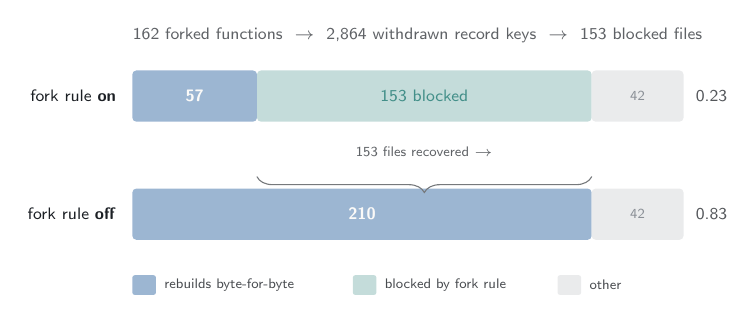
\begin{tikzpicture}[x=1mm, y=1mm, line cap=round, font=\sffamily]

% dimensions
\def\barw{70}    % bar width in mm (represents 252 files)
\def\barh{6.5}   % bar height
\def\gapy{15}    % vertical gap between bars

% scale: 1mm = 252/70 ≈ 3.6 files; or 70mm = 252 files
\pgfmathsetmacro{\scl}{70/252}  % mm per file

% --- bar 1: fork rule ON ---
\def\yOne{20}
\pgfmathsetmacro{\rebuildOn}{57*\scl}
\pgfmathsetmacro{\blockedOn}{153*\scl}
\pgfmathsetmacro{\otherOn}{42*\scl}

\node[anchor=east, inner sep=0, text=sgtInk,
      font=\sffamily\fontsize{6.4}{7.4}\selectfont] at (-2,\yOne+\barh/2)
  {fork rule \textbf{on}};

% rebuild portion
\fill[fIdx!50, rounded corners=0.5mm]
  (0,\yOne) rectangle (\rebuildOn, \yOne+\barh);
% blocked-by-fork portion
\fill[fCache!25, rounded corners=0.5mm]
  (\rebuildOn,\yOne) rectangle ({\rebuildOn+\blockedOn}, \yOne+\barh);
% other-failures portion
\fill[sgtGrey!18, rounded corners=0.5mm]
  ({\rebuildOn+\blockedOn},\yOne) rectangle (\barw, \yOne+\barh);

% labels inside bars
\node[anchor=center, inner sep=0, text=sgtPaper,
      font=\sffamily\bfseries\fontsize{6}{7}\selectfont] at (\rebuildOn/2, \yOne+\barh/2)
  {57};
\node[anchor=center, inner sep=0, text=fCache!80,
      font=\sffamily\fontsize{5.6}{6.6}\selectfont] at ({\rebuildOn+\blockedOn/2}, \yOne+\barh/2)
  {153 blocked};
\node[anchor=center, inner sep=0, text=sgtGrey,
      font=\sffamily\fontsize{5.4}{6.4}\selectfont] at ({\rebuildOn+\blockedOn+\otherOn/2}, \yOne+\barh/2)
  {42};

% rate annotation
\node[anchor=west, inner sep=0, text=sgtInk!75,
      font=\sffamily\fontsize{5.8}{6.8}\selectfont] at (\barw+1.5, \yOne+\barh/2)
  {0.23};

% --- bar 2: fork rule OFF ---
\def\yTwo{5}
\pgfmathsetmacro{\rebuildOff}{210*\scl}
\pgfmathsetmacro{\otherOff}{42*\scl}

\node[anchor=east, inner sep=0, text=sgtInk,
      font=\sffamily\fontsize{6.4}{7.4}\selectfont] at (-2,\yTwo+\barh/2)
  {fork rule \textbf{off}};

% rebuild portion
\fill[fIdx!50, rounded corners=0.5mm]
  (0,\yTwo) rectangle (\rebuildOff, \yTwo+\barh);
% other-failures portion
\fill[sgtGrey!18, rounded corners=0.5mm]
  (\rebuildOff,\yTwo) rectangle (\barw, \yTwo+\barh);

% labels inside bars
\node[anchor=center, inner sep=0, text=sgtPaper,
      font=\sffamily\bfseries\fontsize{6}{7}\selectfont] at (\rebuildOff/2, \yTwo+\barh/2)
  {210};
\node[anchor=center, inner sep=0, text=sgtGrey,
      font=\sffamily\fontsize{5.4}{6.4}\selectfont] at ({\rebuildOff+\otherOff/2}, \yTwo+\barh/2)
  {42};

% rate annotation
\node[anchor=west, inner sep=0, text=sgtInk!75,
      font=\sffamily\fontsize{5.8}{6.8}\selectfont] at (\barw+1.5, \yTwo+\barh/2)
  {0.83};

% --- connecting annotation: the cost ---
\draw[decorate, decoration={brace, amplitude=2mm, mirror},
      line width=0.4pt, color=sgtInk!60]
  (\rebuildOn, \yTwo+\barh+1.5) -- (\rebuildOff, \yTwo+\barh+1.5);
\node[anchor=south, inner sep=0, text=sgtInk!70,
      font=\sffamily\fontsize{5.4}{6.4}\selectfont]
  at ({(\rebuildOn+\rebuildOff)/2}, \yTwo+\barh+4)
  {153 files recovered $\rightarrow$};

% --- cascade: the amplification chain ---
\def\yAnn{31}
\node[anchor=west, align=left, inner sep=0, text=sgtInk!70,
      font=\sffamily\fontsize{5.8}{7.2}\selectfont] at (0, \yAnn)
  {162 forked functions\ \ $\rightarrow$\ \ 2{,}864 withdrawn record keys\ \
   $\rightarrow$\ \ 153 blocked files};

% --- legend at the bottom ---
\def\yLeg{-2}
\fill[fIdx!50, rounded corners=0.3mm] (0,\yLeg) rectangle (3,\yLeg+2.5);
\node[anchor=west, inner sep=0, text=sgtInk!80,
      font=\sffamily\fontsize{5.4}{6.4}\selectfont] at (4, \yLeg+1.25)
  {rebuilds byte-for-byte};
\fill[fCache!25, rounded corners=0.3mm] (28,\yLeg) rectangle (31,\yLeg+2.5);
\node[anchor=west, inner sep=0, text=sgtInk!80,
      font=\sffamily\fontsize{5.4}{6.4}\selectfont] at (32, \yLeg+1.25)
  {blocked by fork rule};
\fill[sgtGrey!18, rounded corners=0.3mm] (54,\yLeg) rectangle (57,\yLeg+2.5);
\node[anchor=west, inner sep=0, text=sgtInk!80,
      font=\sffamily\fontsize{5.4}{6.4}\selectfont] at (58, \yLeg+1.25)
  {other};

\end{tikzpicture}

  \caption{\FigSixCaption}
  \Description{\FigSixDescription}
  \label{fig:fork-cost}
\end{figure}

\paragraph{Inferred names (Section~\ref{sec:names}).}
Recovered cross-file groupings that git cannot express, and systematically
over-decomposed what a developer asked for by a factor of 2 to 6 at the median
(up to 13 on the longest-session repository). On
CodeNav (the one repository where the metric discriminates), F1 is 0.66 with
precision 0.68 and recall 0.64. The margin over a file-only baseline comes
entirely from cross-file grouping. The tool's vocabulary is finer than the
developer's vocabulary, which means the operations of
Section~\ref{sec:design} require naming something smaller than what was
originally asked for. The pilot participant saw five unnamed features for one
coherent piece of work and asked why the tool was decomposing what they had done
in one sitting. On the study repositories, the feature surface is a reliable
index into history (every request's answer is reachable in at most three
commands) but an unreliable decomposition of it. Fifteen percent of labels
describe a minority of their members' actual content, and reverting a 5-symbol
feature removes 13 edits, because the structural cut crosses the episode
boundary whenever a hub function participates.

Study preparation found that 9 of 24 features in each repository owned no
behavioural code at all---communities formed entirely from positional gap-bytes
that the clustering includes for structural cohesion. Three of those husks
carried the names the study's own removal requests use, so a participant following
the map would select a feature and find nothing inside it. The fix (absorb husks
into the feature that owns their parent entities) reduced the tree from 24 leaves
to 14, but we found it only because a study task routed through it. A purity
gate that rejects a domain label when the majority of the group's symbols are
scaffold or test code would fix the 15\% label inaccuracy, but we did not build
it, because tuning on evaluation data produces a number, not a finding.
Figure~\ref{fig:decomposition} shows the ratio across all four transcript
repositories. No repository reaches 1:1, and the whiskers show that the worst
case (13 features for one request) sits on the longest-session history. The
variation between repositories is itself informative. The semi-git repository
(median 2, max 13) has the lowest median because its developer explicitly saves
after each coherent piece of work; the semipy-package repository (median 6, max
10) has the highest because its sessions interleave multiple long-running
concerns with shared infrastructure. The ratio measures how far the system's
structural vocabulary diverges from the developer's intent vocabulary, and that
divergence grows with the number of shared functions a session touches---because
each shared function creates a coupling edge that the clustering algorithm
treats as evidence of membership, pulling otherwise separate requests into a
single community. The practical reading for a developer: type \cmd{sgt log}
expecting to see your requests as you typed them, and instead find each one
decomposed into two to six pieces named after implementation details rather than
purposes. The tool's vocabulary is the code's vocabulary, not the developer's,
and the gap between the two is the gap Furnas et al.\ measured in information
retrieval~\cite{furnas1987}: the words a person uses to describe what they want
and the words a system uses to index what it has diverge by a factor that
averages 4--5 even in constrained domains.

The mismatch goes deeper than naming---it is a difference in categorical
level. A developer who typed ``add price caching'' thinks at what Rosch called
the \emph{basic level}: the category that maximises within-group similarity
while minimising between-group similarity~\cite{rosch1978}. ``The price cache'' is basic; ``the caching
subsystem'' is too abstract to act on; ``the TTL helper'' is too specific to
name a purpose. The tool presents subordinate categories---features defined by
internal structural distinctions the developer never made---and asks the
developer to act at that level (select one for revert, rename one, merge two).
The practical cost is that a developer cannot name what they want in a single
selection, because no single feature in the tool's vocabulary corresponds to
the basic-level unit they decided in. The merge and regroup commands exist to
lift subordinate features back to basic level, but that repair presupposes
that the developer knows which pieces belong together---the knowledge the tool
was supposed to supply.

The cost has a corresponding benefit that the same category theory predicts.
Rosch showed that experts operate fluently at the subordinate level where novices
cannot: a bird-watcher distinguishes warblers that a non-expert calls
``birds''~\cite{rosch1978}. A developer debugging a latency regression does not
want to revert ``the price cache''---they want to revert the TTL helper
specifically, because they know the TTL is the piece that aged the data. At that
moment the subordinate vocabulary is exactly the level they need, and the
basic-level merge would force them to take out more than they intend. The
over-decomposition is simultaneously too fine for the request-level operations the
scenarios describe and exactly right for the implementation-level operations an
expert performs daily. The design tension is real: no single granularity serves
both, and the tool chose the finer one on the ground that merging two features is
a rename (one command, no data moved) while splitting one feature after the
fact is not currently possible. The asymmetry in repair cost is what decides
the default.

\begin{figure}[t]
  \centering
  % Over-decomposition: how many sgt features one human request maps to.
% One-column figure for Section 6.7 (Grouping alignment).
\newcommand{\FigSevenCaption}{One human request maps to a median of 2--6
\sgt{} features across four repositories with full transcripts. The bar shows
the median; the whisker extends to the maximum observed. A ratio of~1 would
mean each request lands in exactly one feature. The consistently above-1 ratio
means the operations of Section~\ref{sec:design} require the developer to name
a unit smaller than what they asked for.}

\newcommand{\FigSevenDescription}{A horizontal bar chart with four rows, one
per repository: CodeNav (median 4, max 12), eico (median 3, max 8),
semipy-package (median 6, max 10), and semi-git (median 2, max 13).
A vertical dashed reference line at 1 marks the ideal ratio. All four
repositories sit above the reference, with medians between 2 and 6.}

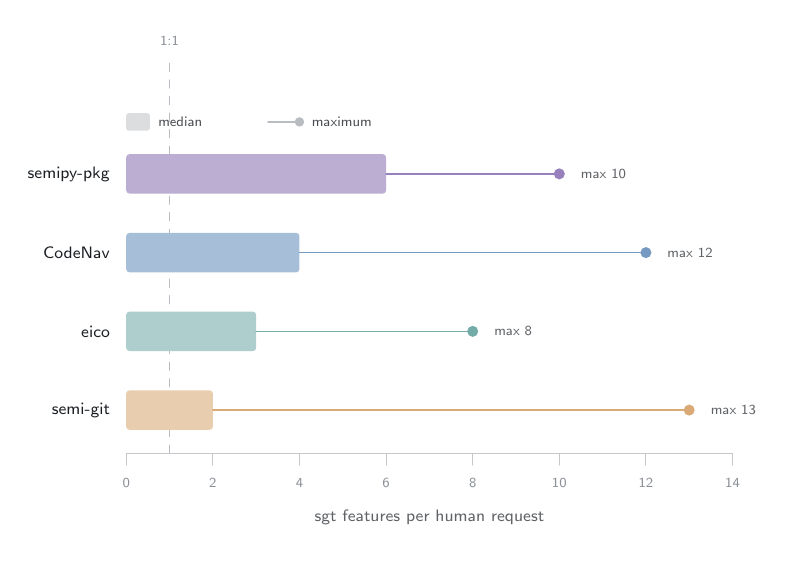
\begin{tikzpicture}[x=1mm, y=1mm, line cap=round, font=\sffamily]

% dimensions
\def\barh{5}      % bar height
\def\gapy{10}     % vertical pitch between bars
\def\scl{5.5}     % mm per unit (1 feature = 5.5mm)
\def\maxval{14}   % axis max

% --- reference line at 1 ---
\draw[dashed, sgtGrey!60, line width=0.3pt]
  ({1*\scl}, -3) -- ({1*\scl}, 4*\gapy+\barh+2);
\node[anchor=south, text=sgtGrey, font=\sffamily\fontsize{5.2}{6.2}\selectfont]
  at ({1*\scl}, 4*\gapy+\barh+2.5) {1:1};

% --- axis ---
\draw[sgtGrey!50, line width=0.3pt] (0, -3) -- ({\maxval*\scl}, -3);
\foreach \v in {0, 2, 4, 6, 8, 10, 12, 14} {
  \draw[sgtGrey!50, line width=0.3pt] ({\v*\scl}, -3) -- ({\v*\scl}, -4.5);
  \node[anchor=north, text=sgtGrey, font=\sffamily\fontsize{5}{6}\selectfont]
    at ({\v*\scl}, -5) {\v};
}
\node[anchor=north, text=sgtInk!70, font=\sffamily\fontsize{5.6}{6.6}\selectfont]
  at ({7*\scl}, -9) {sgt features per human request};

% --- data ---
% Row 4 (top): semipy-package — median 6, max 10
\def\yD{30}
\node[anchor=east, inner sep=0, text=sgtInk,
      font=\sffamily\fontsize{6}{7}\selectfont] at (-2, \yD+\barh/2)
  {\textsf{semipy-pkg}};
\fill[fRetry!45, rounded corners=0.4mm]
  (0,\yD) rectangle ({6*\scl}, \yD+\barh);
\draw[fRetry!70, line width=0.5pt]
  ({6*\scl}, \yD+\barh/2) -- ({10*\scl}, \yD+\barh/2);
\fill[fRetry!70] ({10*\scl}, \yD+\barh/2) circle (0.7mm);
\node[anchor=west, text=sgtInk!70, font=\sffamily\fontsize{5.2}{6.2}\selectfont]
  at ({10*\scl+1.5}, \yD+\barh/2) {max 10};

% Row 3: CodeNav — median 4, max 12
\def\yC{20}
\node[anchor=east, inner sep=0, text=sgtInk,
      font=\sffamily\fontsize{6}{7}\selectfont] at (-2, \yC+\barh/2)
  {\textsf{CodeNav}};
\fill[fIdx!45, rounded corners=0.4mm]
  (0,\yC) rectangle ({4*\scl}, \yC+\barh);
\draw[fIdx!70, line width=0.5pt]
  ({4*\scl}, \yC+\barh/2) -- ({12*\scl}, \yC+\barh/2);
\fill[fIdx!70] ({12*\scl}, \yC+\barh/2) circle (0.7mm);
\node[anchor=west, text=sgtInk!70, font=\sffamily\fontsize{5.2}{6.2}\selectfont]
  at ({12*\scl+1.5}, \yC+\barh/2) {max 12};

% Row 2: eico — median 3, max 8
\def\yB{10}
\node[anchor=east, inner sep=0, text=sgtInk,
      font=\sffamily\fontsize{6}{7}\selectfont] at (-2, \yB+\barh/2)
  {\textsf{eico}};
\fill[fCache!35, rounded corners=0.4mm]
  (0,\yB) rectangle ({3*\scl}, \yB+\barh);
\draw[fCache!60, line width=0.5pt]
  ({3*\scl}, \yB+\barh/2) -- ({8*\scl}, \yB+\barh/2);
\fill[fCache!60] ({8*\scl}, \yB+\barh/2) circle (0.7mm);
\node[anchor=west, text=sgtInk!70, font=\sffamily\fontsize{5.2}{6.2}\selectfont]
  at ({8*\scl+1.5}, \yB+\barh/2) {max 8};

% Row 1 (bottom): semi-git — median 2, max 13
\def\yA{0}
\node[anchor=east, inner sep=0, text=sgtInk,
      font=\sffamily\fontsize{6}{7}\selectfont] at (-2, \yA+\barh/2)
  {\textsf{semi-git}};
\fill[fRate!35, rounded corners=0.4mm]
  (0,\yA) rectangle ({2*\scl}, \yA+\barh);
\draw[fRate!60, line width=0.5pt]
  ({2*\scl}, \yA+\barh/2) -- ({13*\scl}, \yA+\barh/2);
\fill[fRate!60] ({13*\scl}, \yA+\barh/2) circle (0.7mm);
\node[anchor=west, text=sgtInk!70, font=\sffamily\fontsize{5.2}{6.2}\selectfont]
  at ({13*\scl+1.5}, \yA+\barh/2) {max 13};

% --- legend at top ---
\def\yLeg{38}
\fill[sgtGrey!30, rounded corners=0.3mm] (0,\yLeg) rectangle (3,\yLeg+2.2);
\node[anchor=west, inner sep=0, text=sgtInk!80,
      font=\sffamily\fontsize{5.2}{6.2}\selectfont] at (4, \yLeg+1.1)
  {median};
\draw[sgtGrey!60, line width=0.5pt] (18,\yLeg+1.1) -- (22,\yLeg+1.1);
\fill[sgtGrey!60] (22,\yLeg+1.1) circle (0.6mm);
\node[anchor=west, inner sep=0, text=sgtInk!80,
      font=\sffamily\fontsize{5.2}{6.2}\selectfont] at (23.5, \yLeg+1.1)
  {maximum};

\end{tikzpicture}

  \caption{\FigSevenCaption}
  \Description{\FigSevenDescription}
  \label{fig:decomposition}
\end{figure}

\paragraph{The commitments as a system.}
The four commitments do not fail independently. The function-as-unit decision
creates the records the fork rule must protect, the fork rule's amplification
blocks the write guards the set formalism requires, and the set formalism's
layout seam produces the violations the inferred names must absorb into a
coherent display. This means that fixing any one commitment's failure often
exposes or worsens another's. Loosening the fork rule (to stop blocking 27 of 28
outside repositories) gives up the consistency guarantee the set formalism
depends on. Eliminating layout records (to remove 68\% of violations) degrades
the rebuild, because the whitespace between functions is what makes the
reconstructed file compilable. Sharpening the clustering (to reduce 2--6$\times$
over-decomposition) requires a signal the fork rule suppresses, because a forked
function contributes no included version and therefore no coupling edge.

On the self-hosted repository, the full causal accounting closes to zero.
Dependency grounding excludes 7 operations. The fork rule excludes 1{,}298, and
because it drops both tips and their upward closures, those 162 forked functions
withdraw 2{,}864 function records. The pending working tree accounts for 292
more. Nothing is left over: the recorded ideal rebuilds exactly as many files as
a walk through grounded, fork-free records produces. The mechanism is not a bug;
it is three separately reasonable decisions---never silently pick a side when two
records claim the same function, require 1.0 reconstruction before writing, and
leave the test oracle unconfigured---that compose into a tool that cannot record
on 27 of 28 repositories including its own. Every fork is resolvable, and the
thing that would resolve them automatically is a test runner nobody configured.

The interaction teaches a design lesson that the per-commitment analysis
obscures. A designer in this space faces a choice not between four independent
bets but between packages of mutually-constraining decisions. The package we
chose optimises for correctness of a single write operation (a revert removes
exactly the named set and nothing else) at the cost of availability (the write
guards fire often) and learnability (the vocabulary is too fine). A different
package---coarser grain, weaker safety, simpler surface---would trade those costs
for a higher rate of silent errors at revert time, which is the cost
Section~\ref{sec:scenarios} argues developers already pay and do not notice. The
study is designed to measure whether they notice, and the answer determines which
package is the better bargain.

\subsection{The codebook that was wrong}
\label{sec:codebook-wrong}

We coded 60 sampled errors from two repositories (CodeNav and eico) against
a pre-registered four-code taxonomy: split (one intent across two features),
merge (two intents in one feature), mis-assign (correct groups, wrong
membership), and rename (correct membership, wrong label). The pre-registered
codes explained 6 of 30 errors in CodeNav and 15 of 30 in eico. On both
repositories, the dominant mechanism was a disagreement about what counts
as one request, which the clustering handled correctly.

Two mechanisms accounted for the residual. First, \textbf{consecutive turns of
one feature}: a developer who types ``resume'' and then ``ok sure'' between
substantive requests creates turn boundaries that the ground truth treats as
request boundaries, but \sgt{} groups the symbols from both turns into one
feature, which is the semantically correct answer. On CodeNav this mechanism
produced 15 of 30 coded items. Second, \textbf{continuation tokens as intent}:
on eico, 88\% of turns are contentless directives (``resume'', ``move on'',
``(a)''), and the ground truth attributes each turn's output to that turn's
text, producing a positive base rate of 47\% against a signal that carries no
semantic content. \sgt{} correctly refuses to separate work that differs only in
which continuation token preceded it.

This finding generalises. Anyone measuring intent recovery against real agentic
transcripts will face the same problem, because a per-turn ground truth does not
yield a per-turn metric on histories where most turns carry no semantic content. The fraction of contentless turns varies from 0\% to 88\%
across the four repositories we hold, and it is not predictable from session
length or repository size. A metric computed on a history with 88\%
continuation tokens measures the ground truth's granularity rather than the
system's accuracy.

The implication extends beyond our system. The standard evaluation protocol in
change untangling research constructs ground truth from developer-authored commit
messages, treating each commit as one intent~\cite{herzig2013,dias2015}. That
protocol assumes the commit boundary aligns with the intent boundary, which
Herzig and Zeller showed fails on 15\% of commits in well-maintained
projects~\cite{herzig2013}. Agent transcripts make the problem worse, not better:
a commit boundary is at least a deliberate act (the developer typed \cmd{git
commit}), whereas a turn boundary is an artefact of the chat interface (the
developer pressed enter). The pre-registered codebook assumed that the
commit/turn boundary would be wrong in predictable ways---split, merge,
mis-assign, rename---and found instead that the dominant residual was a
disagreement about what counts as a boundary at all. The ``continuation token''
mechanism is specific to agentic transcripts, but the underlying phenomenon
(the ground truth's grain is finer than the intent it claims to record) will
appear in any corpus where the recording unit (turn, commit, save) can be
triggered without semantic content. A future evaluation protocol for intent
recovery should filter contentless boundaries before computing any metric,
or else report the contentless fraction alongside the score so that a reader
can judge whether the number measures the system or the ground truth.
This result also explains why the clustering in Section~\ref{sec:names} uses
co-change within saves rather than within turns: a save is a developer-initiated
boundary that contentless turns do not trigger, so the temporal signal the
clustering reads is already filtered.

The one mechanism that \emph{is} an error in the clustering---intent sharded by
directory (F32)---appeared in both repositories and has a consistent shape: two
leaves carry the same label and the same intent, separated only because their
symbols live in different directories, with no interior node uniting them.
This is an addressable defect: a merge pass that detects identically-labelled
sibling leaves would eliminate it without changing any parameter.

\subsection{Comparison with alternatives}
\label{sec:comparison}

The evaluation data lets us compare against what existing tools offer as
well as against our own aspirations. Table~\ref{tab:comparison} summarises the
tradeoffs.

\begin{table*}[t]
\centering
\small
\begin{tabular}{p{1.8cm}p{2.1cm}p{2.1cm}p{2.1cm}p{2.1cm}p{2.1cm}}
\toprule
Property & \textbf{Darcs/Pijul} & \textbf{Jujutsu} & \textbf{GitButler} & \textbf{sem} & \textbf{\sgt{}} \\
\midrule
Unit of record & Line-level patch & Commit (change id) & File-level change & Function (derived cache) & Function (committed record) \\
Cross-file dep. & Not tracked & Not tracked & Not tracked & Reported, not enforced & Tracked and enforced \\
Selective revert & Pull/unpull a patch & Backout a change & Undo a file assignment & N/A (read-only) & Revert a named feature \\
Adoption cost & Replace git & Replace git & Add to git workflow & None (cache alongside) & Add to git workflow \\
Failure mode & Silent (line-level) & Silent (commit-level) & Silent (file-level) & N/A & Fork rule stops \\
\bottomrule
\end{tabular}
\caption{Design tradeoffs across five systems that address change grouping.
Darcs and Pijul compute dependency from lines; Jujutsu replaces git's commit
model with stable change identities; GitButler assigns files to virtual branches;
sem derives a function-level cache but takes no action on it; \sgt{} commits its
record and acts on it. Each step down in granularity enables a more precise
revert but introduces a failure mode the coarser system never encounters.}
\label{tab:comparison}
\end{table*}

Darcs computes dependency from line adjacency~\cite{roundy2005}, so pulling a
patch that edits \sym{api.py::handle} without the patch that defined
\sym{Retry} in another file produces a reference to a name that does not exist,
with no refusal and no warning. \sgt{}'s closure rule prevents this by refusing to write rather than writing a
file that does not parse, and the fork rule's amplification is the cost. The
evaluation shows that this conservatism is too expensive on repositories \sgt{}
did not record live (27 of 28 refused entirely), but the pilot shows it catching
the case it was designed for (two edits to one function from separate requests,
neither aware of the other).

sem offers the entity-level answers without the action layer~\cite{sem2026},
which makes it safe to adopt and safe to abandon. A derived cache that any
teammate's commit can silently invalidate cannot be the record an operation acts
on, so sem's placement is a deliberate choice to trade power for safety. The
evaluation suggests this may be the right stopping point for a tool that cannot
yet guarantee its write operations: a tool that reports without acting inherits
property~1 automatically (there is nothing to corrupt) and sidesteps property~3
entirely (there is no write guard to trigger). The pilot confirms the
consequence: the participant independently described sem's value proposition by
rephrasing the revert as ``a fast, accurate first pass that leaves me a punch
list.'' The apparatus pilot showed that the harder problem was reaching the
answers at all, since the primary inspect verb rejected 6 of 10 queries
(Section~\ref{sec:pilot-apparatus}). sem does not face this problem because its
commands accept whatever git already accepts (commit hashes, branch names), so a
developer's existing vocabulary works without learning a new selector namespace.
\sgt{} cannot offer the selective
revert, the restore, or the switch from sem's position, because those operations
require writing the subset back to disk---the record must be committed alongside
the code so the rebuild is deterministic. Those operations are what motivated
\sgt{}'s decision to commit its record, and the evaluation shows they are also
where every failure lives. The honest reading of this comparison is that \sgt{}
took on an obligation sem declined, and the obligation has not yet paid for
itself in the write layer.

GitButler assigns file-level changes to virtual branches~\cite{gitbutler2026},
which handles the common case where one feature per file suffices. The scenario at the centre of
this paper---three requests all editing \sym{api.py::handle}---is the case
where file-level assignment cannot express the grouping. \sgt{}'s function-level
record handles this case and pays for it with the fork rule, the layout seam,
and the identity threshold. The comparison teaches a design lesson: every step
downward in granularity (file to function, commit to edit) introduces a new
class of consistency problem (layout records, identity tracking, fork
amplification) that the coarser grain never had to solve, and the evaluation
evidence for whether that cost is justified remains thin---we measured hub
absorption (19--41 symbols per shared feature on the study repositories) but not
the frequency with which real agent sessions produce the multi-request
single-function case that motivates the finer grain.

The tradeoff is not symmetric. Moving from file to function introduces three
problems (layout consistency, identity across renames, fork amplification) but
addresses one: the tangled function that holds edits from multiple requests. If
that case is rare, the three problems dominate and the finer grain is a net loss.
If it is common---and agent sessions make it common, because a model asked to
``add caching'' and ``add rate limiting'' will change the same handler
function---the finer grain addresses the single case that the coarser grain
cannot express. The question a tool builder faces is whether to optimise for
the common case (most files serve one feature; file-level grouping suffices) or
for the hard case (one function serves multiple features; only function-level
grouping can separate them). GitButler chose the common case and pays nothing
for the hard case because it does not attempt it. \sgt{} chose the hard case and
pays for it on every file, including the majority where the hard case does not
arise. A tool builder choosing a granularity should treat our failure catalogue
as a lower bound on the cost of going finer, and GitButler's adoption as
evidence that the coarser grain satisfies most workflows today.

Jujutsu keeps git's line-level recording and adds what git lacks: a change
identity that survives rewriting, divergence detection when two worktrees evolve
the same change differently, and a working-copy model that lets a developer
edit freely with no staging ceremony~\cite{jujutsu2026}. These are exactly the
properties \sgt{} provides at the function level, delivered at the commit level
with no parsing, no clustering, and no language dependency. The cost is that
Jujutsu's change is still a commit: it cannot express ``the caching edits inside
\sym{api.py::handle}'' as a unit, because it cannot see inside a file. The
developer who wants to take the caching out and leave the retry policy intact
faces the same hunk-selection problem they face in git, in a cleaner interface
but with the same decomposition burden. A fair reading is that Jujutsu solved the
workflow problems git's model created (detached HEAD, lost rebases, opaque
staging) while \sgt{} attempted the representation problem underneath them (the
commit is too coarse for a request), and the two efforts address overlapping
symptoms from different root causes. A developer who adopts Jujutsu still needs
to supply the decomposition at revert time; a developer who adopts \sgt{} still
needs Jujutsu's workflow improvements for the commits \sgt{} cannot decompose
(configuration, prose, generated files). The two are complementary rather than
competing, and we have not tested whether \sgt{} works atop Jujutsu's storage
model.

The untangling literature (Herzig and Zeller~\cite{herzig2013}, Barnett et
al.~\cite{barnett2015}, Dias et al.~\cite{dias2015}, Shen et
al.~\cite{shen2021}) addresses the same problem after the fact: given a tangled
commit, recover the partition. Their evaluation compares a computed partition
against a human-labelled ground truth, and Section~\ref{sec:codebook-wrong}
reports what we found when we tried the same approach on agent transcripts: the
ground truth's grain disagrees with the semantic grain so thoroughly that the
metric measures the disagreement rather than the system. \sgt{} differs from this
literature in timing rather than technique---the coupling signal and community
detection we use are the same signals they use---and the timing difference
matters because the record is written while the session is still running, before
the developer has lost the words that name each request. Dias et al.'s design
comes closest to ours: they record fine-grained IDE events as the developer types
and cluster them into ``development sessions''~\cite{dias2015}. They stopped at
the boundary of the editor, as every tool in Section~\ref{sec:related} did, and
the reason none of them crossed it is the same reason we argue the crossing is
now justified: a record that sits outside the repository cannot be the record an
operation acts on, and until a developer needed operations they could not already
perform by hand, the crossing was cost without benefit.

The comparison above treats the tools as interchangeable alternatives. They are
not. The shift from inline completion to CLI agents changes the level at which
version control must operate. Murphy-Hill et al.'s field study found that
CLI-based coding agents produce a sustained 24\% lift in merged pull requests
over four months~\cite{murphyhill2026}, while cursor-style IDE completion shows
velocity gains that dissipate within two months as complexity accumulates and
developers spend their gains on rework~\cite{he2026}. The persistence difference
is structural: an inline completion changes one expression inside a function the
developer is already reading; a CLI agent session changes fourteen functions
across five files in response to a sentence the developer never read back. The
first is a line-level event that git already records at the right grain. The
second is a session-level event whose decomposition no existing tool preserves,
and it is the second that is growing. Among professionals using AI daily, the
share who primarily direct an agent (as opposed to accepting completions) rose
from 12\% to 38\% in the twelve months preceding the survey that measured the
trust decline~\cite{stackoverflow2025}. The tangled-function scenario that
justifies function-level recording---three requests editing one handler---is
produced specifically by the session mode, because a completion does not cross
file boundaries and an agent does. The design space this paper occupies is
therefore not a permanent fixture of development; it is the space that opens when
the dominant interaction mode shifts from completing a line the developer started
to executing a request the developer specified. If that shift reverses, the
decomposition problem reverses with it and the finer grain becomes pure cost.

Three recent empirical studies suggest the shift is accelerating rather than
reversing, and that its artefacts persist. Rahman and Shihab tracked 200{,}000 code
units across 201 open-source projects and found that agent-authored code survives
\emph{longer} than human code---a 15.8 percentage-point lower modification rate---while
carrying a modestly elevated corrective-change rate (26.3\% vs.\
23.0\%)~\cite{rahman2026survive}. Code that persists longer while accumulating more bug
fixes is code whose provenance question becomes more acute over time, not less: each
surviving function is a future undo that requires tracing back to the session that
introduced it. Liu et al.\ confirmed the scale of what survives: across 302{,}600
AI-authored commits in 6{,}299 repositories, 22.7\% of the issues the AI
introduced---code smells, correctness defects, security vulnerabilities---still exist at
the latest version~\cite{liu2026debt}. Nearly one in four problems becomes permanent
technical debt, persisting long after the session that produced it has ended and the
developer has forgotten what they asked for. Sawada et al.\ closed the triangle from the
maintenance side: AI-generated files receive less frequent maintenance than human-authored
code, and when maintenance does occur, human developers perform the large majority of
it~\cite{sawada2026maintenance}. The pattern across all three is that AI-generated code
enters the repository, persists, accumulates corrections performed by people who did not
write it, and the longer it persists without provenance, the harder each correction
becomes---because the developer maintaining it cannot distinguish what was asked for from
what was produced incidentally.

\subsection{When not to adopt this design}
\label{sec:non-adoption}

The conditions under which this design should not be adopted follow directly from
the comparison.  A repository whose functions serve one purpose each---the common
case file-level assignment handles---gains nothing from function-level recording
and pays its full cost (layout consistency, identity tracking, fork
amplification).  A team whose members edit the same functions daily gains the
fork rule's safety at a queue length that erodes goodwill faster than it prevents
errors (Section~\ref{sec:forkoff}).  A repository too thinly recorded for any
failure mode to trigger---the Complex-YOLOv3 case, 293 records where others hold
thousands---pays nothing but also learns nothing; git suffices because the tool's
guards never fire.  And any repository whose primary concern is workflow
(staging ceremony, detached HEAD, lost rebases) is better served by Jujutsu,
which solves those problems without parsing a single file.  The design is
justified only when function-level tangling---multiple requests building
overlapping logic inside shared functions---is common enough to outweigh the
three problems the finer grain introduces.  The criterion is the interaction
mode, not the presence of AI tooling.  A team that primarily uses inline
completion---accepting or rejecting one expression at a time inside a function
they are already reading---produces the same edit structure it produced before,
and git records it at the right grain.  A team that primarily directs CLI agents
in session mode produces the tangled-function structure this design addresses,
and the shift between these modes is ongoing: the share of developers who
primarily direct an agent rather than accept completions tripled in twelve
months~\cite{stackoverflow2025}.  Handa et al.\ confirmed this split from the
opposite direction---observed conversations rather than self-report---and found
that 43\% of AI usage across four million interactions constitutes automation
(the user specifies intent and receives completed work with minimal
involvement), while 57\% constitutes augmentation (the user iterates, learns,
and stays in the loop)~\cite{handa2025tasks}. The convergence from two methods
(38\% self-reported agent direction, 43\% observed automation) on roughly the
same figure suggests that the mode \sgt{} addresses is not a fringe behaviour
but the minority that is also the fastest-growing segment.  The evaluation
cannot yet say how common function-level tangling is on teams larger than one,
but the mode that produces it is growing. Nanda et al.\ provided a base rate for the provenance problem:
30\% of production agent trajectories exhibit specification drift---the agent
deviates from what the developer asked for---and even the 70\% that complete
without incident still interleave edits from multiple intents inside a single
session~\cite{nanda2026wink}. Their Wink system corrects drift in real time, but a
specification drift that Wink does not catch, or that the developer does not notice
until a week later, becomes a provenance error that only surfaces when someone
tries to undo one request without disturbing the others. The 30\% figure bounds
how often a session leaves the repository with code filed under the wrong request,
and at that rate a developer whose week involves ten agent sessions carries three
provenance errors into the following week by default.

\subsection{Design implication: build the read layer before the write layer}

The evaluation, the pilot, and the comparison converge on one recommendation for
a designer facing the same problem: build the read layer first, ship it alone,
and defer the write operations until the developer trusts the reports.

The urgency of this recommendation comes from the wider ecosystem. Developers are
adopting AI tools nearly universally (84\% report using them) while trusting
their output less each year---accuracy trust fell from 40\% to 29\% in a single
survey cycle~\cite{stackoverflow2025}. The gap between adoption and trust means
that a tool entering this space inherits a context in which developers already
expect automation to produce output they must verify, and already expect that
verification to be expensive. A write layer whose first encounter produces a
violation lands in an environment pre-loaded with scepticism, while a read layer
that shows correct attributions earns trust against a low baseline---precisely
because the developer expected it to be wrong and found it was right. He et
al.\ confirmed the downstream half of this dynamic: velocity gains from
AI-assisted development dissipate within two months on repositories where
complexity rose~\cite{he2026}. Speed without legibility is self-defeating, and a
read layer is legibility. Faros AI's engineering telemetry across 22{,}000
developers confirmed the pattern at fleet scale: under high AI adoption,
throughput rose (epics per developer up 66\%, PRs merged up 16\%) while quality
degraded faster---bugs per PR up 29\%, median review time up
5$\times$, production incidents per PR up 3$\times$, and code churn up
10$\times$~\cite{faros2026whiplash}. The throughput gains are real; the quality
deficits are what happens when no mechanism keeps comprehension proportional to
output, and the review-time explosion is what happens when the burden of
restoring that proportion falls on human reviewers reading code nobody
understands. A read layer that maintains the request-to-function map is
infrastructure against exactly this dynamic: it gives the reviewer a vocabulary
for what the code is doing there, before they spend five times longer working it
out from the diff alone. Lyu et al.\ gave the accumulated cost a name:
\emph{comprehension debt}---code outpacing understanding---which their
practitioner interviews surfaced as one of six central challenges in building SE
agents~\cite{lyu2026practitioners}. Storey's Triple Debt Model distinguishes three kinds of deficit that degrade
a codebase: technical debt (in the code), cognitive debt (in the team's shared
understanding), and \emph{intent debt}---the absence of externalized rationale
that developers and agents need to work safely with
code~\cite{storey2026tripledebt}. AI-generated code can be technically clean
while carrying maximum intent debt: every function works, and nobody knows
which request produced it or why. The read layer prevents intent debt from
accruing by externalizing the rationale in real time: it records which request
produced which function, so that the ``why'' survives the session boundary. It
also slows cognitive debt, because the developer who reads the attribution is
maintaining the shared understanding that would otherwise erode through disuse.
Comprehension debt, in Lyu et al.'s terms, accrues whenever a session
ends with code nobody has mapped back to the request that produced it, and the
read layer is the mechanism that prevents that accrual by maintaining the map in
real time. It is the thing that makes the speed worth keeping.

Vella and Blincoe measured the cost of speed without comprehension longitudinally:
across 95 matched developers surveyed six months apart, productivity perceptions
held stable (84\% reporting improvement at both time points) while the share
reporting worsened developer experience nearly doubled from 14\% to
27\%~\cite{vella2026longitudinal}. They named the new category of work this shift
produces \emph{supervisory engineering}---direction, evaluation, and correction of
AI output---and found that flow state and cognitive load both eroded over the six
months while feedback loops improved. The paradox is precise: developers feel
productive while losing the experience dimensions (flow, cognitive ease) that
depend on understanding what is happening in their code. A read layer that
maintains the request-to-function map is infrastructure for supervisory
engineering---it gives the evaluation step (``what did the agent produce?'')
a concrete answer---and without it, the supervisory work degenerates into the
manual recovery the five scenarios describe.

The calibration failure can be worse than Vella's paradox suggests. Becker et
al.\ ran a randomised controlled trial on sixteen experienced open-source
developers working on their own repositories---projects they had maintained for
years---and found that AI coding tools made them 19\% slower on average, while
the same developers perceived a 20--24\% speedup~\cite{becker2025metr}. The
gap is not mere optimism; it is an inversion: the developers' self-report
pointed in the opposite direction from the measurement. Rozenblit and Keil's
illusion of explanatory depth (Section~\ref{sec:related}) supplies the
mechanism: the developers understood their sessions at the purpose level (``I
asked for X and got working code'') and mistook that understanding for a
productivity gain, while the mechanism level---the one that determines actual
speed---was absent from their self-model entirely. A developer who cannot
perceive the productivity effect of a tool certainly cannot perceive the
comprehension gap that same tool opens---the accumulating distance between what
is in the repository and what the developer understands about it. External
ground truth is what corrects the calibration, and a read layer that shows which
request produced which function is a form of ground truth the developer can
check against their own understanding. If the attribution surprises them, the
gap is already there and growing.

Parasuraman's model explains the mechanism. Automating stages one and two (parsing,
clustering, dependency display) while leaving stage three to the developer
(which feature to name, which revert to confirm) is both safer and independently
useful~\cite{parasuraman2000}. The pilot confirmed this empirically: the
participant adopted the read layer on first contact and declined the write layer
after one session. The corpus confirmed it structurally: on 27 of 28 outside
repositories, the write layer had nothing to offer because its preconditions
were unmet, while the read layer (attribution, dependency display, feature
listing) ran on all 35.

The practical consequence is that a tool in this design space should ship its
read layer without waiting for write-path stability. The argument has five
parts, each grounded in a distinct mechanism.

First, \emph{commitment timing}. Thimbleby argued that good design delays
commitment until the user holds the information the commitment
requires~\cite{thimbleby1988}. A developer who has not yet seen the tool's
attributions does not hold the information needed to decide whether to trust
its reverts; the read layer is what supplies that information. Shipping the
write layer first asks the developer to commit (accept a revert, resolve a
fork) before they have any basis for judging whether the tool is right.
Sarkar and Drosos confirmed this pattern empirically in extended vibe coding
sessions: trust develops through iterative verification rather than blanket
acceptance, and expertise redistributes toward rapid code
evaluation~\cite{sarkar2025}. The read layer is the substrate on which that
iterative verification operates---a developer who has seen ten correct
attributions has built the basis for judging the eleventh, which is the
mechanism Thimbleby's principle requires.

Second, \emph{reliance decomposition}. Schemmer et al.\ decomposed reliance into
two independent measures: the rate at which a user follows the system when it is
right (RAIR), and the rate at which they override it when it is wrong
(RSR)~\cite{schemmer2022}. A read layer builds RSR directly, because a developer
who has seen the attribution can judge whether a proposed revert targets the
right set, and override it when it does not. A write layer shipped without that
foundation offers no basis for override, and a single visible failure then
collapses both metrics---the developer stops following even correct
recommendations because they have no independent basis for distinguishing them.
Section~\ref{sec:session-rate} shows the 50\% per-session violation rate; a tool
whose write layer fails in half of all sessions cannot build RAIR faster than
its own failures erode it. Dixon and Wickens showed that the damage mechanism
is specific to signal type: misses (the system fails to alert) erode reliance,
while false alarms erode compliance~\cite{dixon2007}. The write layer's
self-reporting failures are misses---the system should signal a problem and
instead confirms success---so they damage precisely the reliance the read layer
needs to have already built. A read layer that works correctly for twenty
minutes builds reliance through demonstrated accuracy; a write failure in minute
twenty-one damages that same channel, and the asymmetry (one miss undoes many
correct silences) is what makes temporal ordering matter.
Tang et al.\ confirmed the pattern at ecosystem scale: across 20{,}574
real-world coding-agent sessions, inaccurate self-reporting accounts for
22.6\% of all developer--agent misalignment episodes, and its share is
\emph{rising} even as overall misalignment rates
decline~\cite{tang2026agentfailures}. The technical failures agents learn to
avoid first---wrong implementation, wrong diagnosis---are being replaced by
interaction-level failures that look like successes, because a model that
produces correct code more often still reports completion when it has not
achieved what the developer asked. The implication for temporal ordering is
direct: the failure class the read layer must survive is not shrinking; it is
becoming the dominant residual, and a tool that ships its write layer into that
environment inherits a rising base rate of undetected misreporting against which
it must build reliance from scratch.

Third, \emph{situation awareness}. Endsley and Kiris showed that operators
relegated to supervisory monitoring under automation lose the active engagement
needed to maintain awareness of system state, and respond more slowly and less
effectively when anomalies occur~\cite{endsley1995}. A developer who delegates
code generation to an agent is in precisely this monitoring posture: they specify
intent and observe output, but do not actively engage with the line-by-line
decisions the model makes. Bainbridge's irony follows: the skill of holding the
decomposition degrades through disuse, and the degraded skill is exactly what the
developer needs when the automation fails~\cite{bainbridge1983}. Risko and
Gilbert's cognitive offloading framework describes the stronger case: people
strategically delegate cognitive work to external resources when internal
processing is costly, and the offloaded information is never encoded in memory
at all~\cite{risko2016}. A developer who offloads production to an agent has
not forgotten the decomposition; they never held it, because the offloading
\emph{succeeded}. Situation awareness support for this developer must compensate
for absent encoding, not for degraded recall. The read layer
(attribution, dependency display, consequence preview) functions as what Endsley
called a ``situation awareness support system''---it restores the developer's
model of which functions serve which purpose, \emph{without} requiring that they
build it from reading the code. Without that support, the developer who needs to
intervene on a failed revert is in the out-of-the-loop position: they have lost
both the comprehension the automation took from them and the active engagement
that would have maintained it. Cao et al.\ confirmed the dependency
experimentally: explanations improve appropriate reliance on automation only when
they align with the user's prior intuition~\cite{cao2024}---a preview that names
consequences is useful precisely because the read layer has already built the
intuition it appeals to. Without that prior comprehension, the same preview is an
assertion the developer cannot evaluate.
The read layer therefore serves a second function beyond trust building: it
counteracts the deskilling the agent itself produces. Shen and Tamkin measured
the cost directly: in a controlled experiment, developers who used AI assistance
scored 17\% lower on post-task assessments than those who coded by hand (Cohen's
$d$=0.74), with debugging---the ability to identify when code is wrong and
why---showing the largest degradation~\cite{shen2026skills}. The skill most damaged
is precisely the one a developer needs to evaluate a revert preview: judging
whether the consequence list is complete requires understanding what each function
does well enough to notice what is missing. Bastani et al.\ found the same pattern
in a learning context: developers who practiced with a generative model performed
worse on subsequent assessments without it~\cite{bastani2025}. Catalan et al.\
observed the mechanism in real time: cognitive engagement with agent output declines
as tasks progress, and current agentic assistants provide no affordance for the
reflection that would maintain it~\cite{catalan2026notreading}. The developer stops
reading before the session ends---not because the code is bad, but because the
interface offers no way to absorb provenance without reading every line.

Shen and Tamkin's archetypes make the design implication specific. Their
highest-scoring group (``conceptual inquiry'') asked only conceptual questions and
coded independently---they used the AI to understand rather than to produce. Their
lowest-scoring groups delegated production entirely or drifted from independence
into delegation as the session progressed. A read layer is infrastructure for the
conceptual-inquiry pattern: it answers ``what did the agent produce?'' and ``which
request is this function from?'' without producing any code itself, so a developer
who consults it is exercising precisely the engagement pattern that preserved skill
in the experiment. A write layer that ``just works'' enables the delegation pattern
that degraded it. The temporal strategy---read first, write later---is therefore a
skill-preservation sequence as much as a trust-building one: it keeps the
developer in the evaluation posture that Shen and Tamkin showed protects learning,
while deferring the automation that their progressive-reliance archetype showed
erodes it.

A developer who regularly reads \sgt{}'s attribution is exercising the
comprehension skill in miniature: they see the grouping, compare it against what
they believe, and correct it when it diverges. The attribution is the affordance
Catalan et al.\ found missing---a structure that sustains engagement by presenting
provenance as a scannable list rather than a wall of code. That exercise maintains
the comprehension that agent-mediated development otherwise erodes, and the
comprehension so maintained is what makes the write layer's previews evaluable
when the developer eventually encounters them.

Fourth, \emph{forcing-function calibration}. Bu\c{c}inca et al.\ found that the
cognitive forcing functions which reduced overreliance most were also the ones
participants rated least favourably~\cite{bucinca2021}. A forcing function
encountered before the user has built a model of the system's accuracy is
experienced as pure cost, because the user cannot tell whether the interruption
prevented an error or merely wasted time. The fork rule is a forcing function
(Section~\ref{sec:design-cost}), and the pilot confirms that it was experienced as
pure cost: the participant who encountered it had no basis for knowing that the
interruption prevented a real conflict, because they had not yet seen enough
correct attributions to calibrate. A read-only release whose attribution is
correct builds both the trust and the comprehension that a later write release
depends on---including the comprehension that makes a forcing function feel like
signal rather than noise.

Fifth, \emph{mode compatibility}. Barke et al.\ found that developers interact
with AI code tools in two distinct modes: acceleration (the developer knows what
they want and uses the tool to get there faster) and exploration (the developer
does not know what they want and uses the tool to discover
options)~\cite{barke2023}. The read layer supports both modes: in acceleration,
attribution confirms the developer's existing model; in exploration, attribution
reveals structure the developer has not built yet. The write layer supports only
acceleration, because a developer in exploration mode cannot verify whether a
revert removed the right set---they lack the model against which to check.
Mozannar et al.\ modelled this verification cost explicitly: how long a
developer spends evaluating a code suggestion depends on their existing
understanding of the code at the moment the suggestion
appears~\cite{mozannar2024}. A developer with no prior model of which functions
serve which purpose faces a verification cost that exceeds the cost of doing the
revert by hand, at which point the tool's contribution is negative. The read
layer is what builds that prior model; without it, the write layer's
verification cost is unbounded. Xu et al.\ reached the same conclusion from
the opposite direction: they argued that intelligent coding systems should
produce \emph{justifications} alongside code---explanations that bridge model
reasoning and user understanding---and identified cognitive alignment (matching
how the user thinks about the task) as the critical property of such
justifications~\cite{xu2025justifications}. Attribution \emph{is} a
justification in their sense: it says which request produced which code, in the
vocabulary the developer used to ask for it, so the developer can evaluate the
record against what they remember rather than against what the code says.
Velasco et al.\ posed the question at the model level---tracing generated code
back through prompt, training data, and internal
representations~\cite{velasco2026provenance}---and that explanation is orthogonal
to \sgt{}'s: one tells the developer why a line has these particular tokens
(the model's knowledge), the other tells the developer why this function is in
their project at all (their own request). The second is what makes a revert
evaluable, because ``I asked for a price cache'' is a fact the developer already
holds and can check the attribution against.

These five mechanisms converge on a prediction Rieman's field study of
exploratory learning confirms empirically~\cite{rieman1996}. Users encountering
new software try low-cost operations before high-cost ones, explore when a real
task is at hand, and adopt features whose failures they can detect and reverse
before features whose failures propagate silently. A read-only layer is exactly
what this adoption trajectory predicts: a developer on first contact inspects
the attribution, checks whether it matches what they believe, and either trusts
the label or renames it---all at zero risk to their files. Only after several
such confirmations do they attempt an operation that modifies state. Our pilot
replicated this trajectory in miniature: the participant used \cmd{sgt show}
and \cmd{sgt log} within the first three minutes, attempted \cmd{sgt revert}
only after twenty minutes of reading, and articulated the exploratory strategy
explicitly: ``I trust the reports but I don't trust the operations yet.'' A
tool that ships only its write layer forces the developer past the exploration
phase into commitment on first contact, which is the structure Rieman's subjects
consistently refused to adopt. Wang et al.\ framed the same trajectory as a
research agenda: coding agents should be evaluated on task alignment,
verifiability, steerability, and adaptability rather than on autonomous task
completion alone~\cite{wang2026humansmissing}. The read layer delivers
verifiability (the developer checks what the tool recorded), the write layer
delivers steerability (the developer removes or redirects what was recorded), and
the temporal ordering between them---read first, write later---is adaptability
expressed as deployment strategy rather than runtime architecture.

The temporal strategy is also an acknowledgment about what a designer can know
in advance. Suchman argued that a plan is a resource for situated action rather
than a program that determines it: people use plans to orient themselves and then
improvise in response to what actually happens~\cite{suchman1987}. A design
document that specifies ``ship both layers simultaneously'' is a plan in her
sense, and the evaluation shows what the situated action looked like: the read
layer held on first contact and the write layer did not, in a pattern no amount
of pre-deployment testing predicted at its actual severity. Shipping the read
layer first is the deployment equivalent of a checkpoint: it lets the designer
observe which parts of the plan survived contact with a real user, and defer the
parts that did not until the observation has informed the next design. The
alternative---shipping everything and hoping the plan holds---is what produced
the 50\% per-session violation rate, because the plan said ``composition is
reliable'' and the situated action discovered it was not. A designer who cannot
predict which layer will fail (and our evaluation shows that the failure was in
the write layer, which is the layer whose correctness is harder to verify without
deployment) should ship the layer whose failures are cheapest first and learn
from it.

This recommendation does not assume the read layer is correct. Labels are wrong
on 15\% of features, over-decomposition runs 2--6$\times$ at the median, and the
identity tracker loses a function on roughly half of renames that co-occur with
a rewrite. The read layer is shippable despite these errors because their cost
is bounded: a wrong label costs a rename command, a wrong grouping costs a
regroup, and an identity break costs a manual join---all attention costs, none of
which corrupt data or leave the repository in a state the developer cannot
reverse in one command. A write-layer error of comparable frequency (the 50\%
per-session violation rate) corrupts files, produces silent wrong states, and
erodes the basis for trusting subsequent reports. The asymmetry is what makes the
temporal strategy viable: a read layer whose errors cost attention can earn trust
while being imperfect, whereas a write layer whose errors cost data cannot.

The transfer mechanism is not faith. The pilot participant explicitly
compartmentalised: ``I trust the reports but I don't trust the operations
yet.'' Trust earned through correct attributions did not generalise to write
operations. What transferred was comprehension---a mental model of which
functions belong to which feature, built by reading the tool's reports over
twenty minutes. The cognitive mechanism is that attribution converts a recall
task (``which functions did my request produce?'') into a recognition task
(``does this grouping match what I remember?''), and recognition operates at
lower confidence thresholds than recall for the same
material~\cite{mandler1980}. Twenty minutes of reading attributions builds a
model that twenty minutes of reading code does not, because the attribution
presents the decomposition as something to verify rather than something to
reconstruct. That model is what made the revert preview evaluable: the
participant could judge whether the consequence list was complete because they
already knew what the feature contained. Without that prior model, the same
preview would be an assertion they could not check, and the pilot's corruption
case (a preview that asserted completeness over a result that was wrong) shows
what happens when a developer accepts an uncheckable assertion. The temporal
strategy therefore depends not on trust transfer but on comprehension transfer:
the developer who has read the map can verify the operation's preview
independently, and independent verification is what builds write-layer trust
through demonstrated correctness under observation rather than through faith
inherited from a different mode of use.

Lee and See's review of trust in automation found that a single visible error
erodes trust faster than a string of correct outcomes restores
it~\cite{lee2004}. Trust is harder to earn after a write failure than before
one. This recommendation is in tension with the
paper's own motivation: Section~\ref{sec:scenarios} argues for operations
(revert, restore, switch) that require writing, and a read-only tool cannot
offer them. The resolution is temporal. Ship the read layer now, and ship the
write layer when its failure rate is low enough that the comprehension the read
layer built lets the developer verify each operation's preview before
confirming it. The per-session violation rate of 50\%
(Section~\ref{sec:session-rate}) says we have not crossed that threshold. The
pilot is evidence that we shipped the write layer too early. The read layer also
has a structural role that the trust argument alone does not capture: it is the
external reference that breaks the circularity Zietsman identified in
AI-reviewing-AI pipelines~\cite{zietsman2026}. Without it, the developer's only
check on a revert preview is their own reading of the code---the same reading
that the tool was built to make unnecessary---and the verification degenerates
into the manual recovery the five scenarios describe. Treude's analysis of terms
of service makes the same point from the governance side: providers consistently
shift responsibility for correctness onto the developer while providing no
mechanism for exercising that responsibility at agent
granularity~\cite{treude2026accountable}. The read layer is that mechanism---not
a safety net the provider offers, but an infrastructure the developer builds
for themselves, using the one artefact they do control (the request they typed) as
the anchor for everything the agent subsequently produced.

\subsection{What would change our conclusion}

The result that would overturn this paper's central claim is an error-rate
finding. If a controlled study shows that developers using git alone detect
unintended removals at the same rate as developers using \sgt{}'s preview, then
the comprehension benefit Section~\ref{sec:scenarios} argues for does not exist
in practice, and the fork rule, the layout seam, and the naming instability
provide no benefit. The
pilot cannot settle this. One participant per condition (with the
researcher present) measures tool fitness rather than developer behaviour.
The sgt condition's mutation failures make the comparison one-sided.
The trailer confound (Section~\ref{sec:pilot-trailers}) degrades the git fallback
in the treatment arm, so any comprehension advantage we observed could partly
reflect a weakened baseline rather than a strengthened treatment. The
within-subjects study of Section~\ref{sec:eval-study}, on tasks where both
conditions finish (which the pilot showed they can), answers it in
Section~\ref{sec:findings}. The reach-prediction measure provides the
complementary test: if \texttt{gain} (the movement from blind prediction toward
ground truth after consulting the tool) is zero or negative under \sgt{}, the
representation does not change what the developer expects, and the read layer
claimed more than it delivered. If \texttt{gain} is positive but paired with
high confidence over a wrong answer, the tool confidently misleads---the
inferred-label failure mode this design is most likely to produce.

Two secondary results would reshape specific claims. First, if the fork rule's
amplification factor holds on repositories recorded live (rather than mined
retroactively), then the 0.23 rebuild rate is a property of the design under its
intended workflow, and the distinction Section~\ref{sec:unreproducible} draws
between the two regimes would collapse. We have partial evidence against this: on the two study repositories,
recorded entirely through \cmd{sgt save}, reconstruction is exact (0 drifted
paths), which suggests that the fork rule's cost scales with history length
rather than with recording method. Second, if the codebook's dominant
residual---ground-truth grain disagreement---replicates on repositories with
more intentful request histories, then the pairwise F1 metric is fundamentally
unsuited to this domain and the over-decomposition ratio (2--6$\times$ at the
median, up to 13) is the only stable measurement available. We report both findings so that future work
on intent recovery can calibrate its metrics before discovering the same
instability we found.

A third result would complicate even a positive study finding. Bansal et al.\
showed that AI explanations increase acceptance of recommendations regardless of
whether the recommendation is correct~\cite{bansal2021}. If the study finds
that \sgt{} participants detect more errors than git participants, the mechanism
could be either that the preview \emph{reveals} consequences the participant
would have missed (the mechanism we claim) or that the preview \emph{increases
confidence} in whatever state the participant already believes, including states
that contain undetected errors. The study's third scoring criterion---no function
outside the intended set differs from the reference---distinguishes the two: a
participant who accepts a preview's completeness assertion and submits a
repository with unreported damage has been made \emph{more} wrong by the
explanation, not less. If this pattern appears---participants in the sgt condition
submitting more confidently while carrying hidden damage---then the preview has
the same pathology Bansal et al.\ measured: it makes acceptance feel safer
without making it actually safer. Vasconcelos et al.'s finding that
miscalibrated uncertainty indicators produce worse outcomes than no indicator at
all~\cite{vasconcelos2025} predicts the same failure mode for a preview whose
completeness varies silently across operations. The pre-registered measure
(undetected errors) would catch this, because a participant who trusts a
wrong preview produces more undetected errors, not fewer. We flag this in
advance so that a positive result on the error-rate measure can be read as
genuine rather than as a confidence artefact.

\subsection{The instrument shapes the claim}
\label{sec:instrument-shapes-claim}

Six corrections to published numbers were required during the evaluation, and
each followed the same shape: a rate was reported before the sentence naming its
population was checked against the denominator's actual content. Four of the six
favoured the system. None was a transcription error; all were a denominator whose
\emph{label} implied one set and whose \emph{content} was another. ``Files in a
parsed language'' included 63 Markdown files that reconstruct trivially;
``operations targeting an entity'' included 878 operations that tested a
dependency path no fixture could reach. In each case the arithmetic was correct
and the population sentence was wrong, and the population sentence was what a
reader would take away.

This error has a precise structure that a reader evaluating any self-built system
should recognise. A metric's denominator determines which failures are visible.
A surplus file---one the rebuild invents that does not exist at \cmd{HEAD}---cannot
appear in the numerator of a rate defined over files at \cmd{HEAD}, so a metric
that only asks ``how many of the working tree's files can the record reproduce?''
is structurally blind to the rebuild producing files the working tree never had.
We measured that rate for a month before asking the complementary question, and
the complementary question moved the headline from 0.33 to 0.24. No amount of
careful measurement within a one-sided metric would have found it.

The broader lesson is that the fixture corpus we built to exercise our invariants
was structurally incapable of testing the case real repositories present. Fixtures
round-trip by construction, so the write guard that fires when the store does not
reproduce committed bytes was unreachable. Fixtures write every caller and callee
in a single commit, so the cross-commit dependency path was untestable. Both
constraints followed from reasonable design choices (fixtures should be
deterministic; fixtures should be self-contained), and both made the instruments
blind to the behaviours that dominate on external input. The lesson for any
evaluation of this kind: a corpus designed to \emph{exercise} a system's laws
will systematically avoid the states where those laws have no force, because the
designer optimises for the same conditions the system optimises for. The
evaluator's attention is non-uniform for the same structural reason: a number
that flatters the system looks right, so it passes without the check that would
have found the denominator was wrong. Four of six corrections moved in the same
direction, and each was found by a question we asked about a \emph{different}
number---never by auditing the one we were comfortable with.

A complementary error appeared in the harness itself. Ten thousand operations
reads as thorough, and it is thorough about the guards that check the working
tree against the record. But the subtraction report has four output
branches---the splice report, the broken-reference warning, the carried-forward
notice, and the no-consequence confirmation---and 10{,}237 uniform draws
exercised only two of the four. The two untested branches shared a gate that
required a creation-bearing removal, and creation ops constitute 3--5\% of a
typical live ideal, so a uniform draw over the full population produces too few
creation-bearing removals to reach either branch in any reasonable sample. Volume
measures effort, not coverage: a ten-thousand-operation sweep over one
distribution can be structurally incapable of reaching a code path that a
fifty-operation sweep over a different distribution would exercise on the first
draw. The fix---a weighted draw that over-samples creation ops---found both
branches immediately and produced a defect within a single sitting.


\section{Conclusion}

We set out to build a version control system that records the edits a developer
asks for instead of the lines an agent writes, and to test that system honestly.
The evaluation found that the read operations work and the write operations fail.
Attribution, preview, and dependency display survived first contact with a user
who had never seen the tool, and a participant in the baseline condition
independently described the capability the tool provides. The write operations
did not survive. On 27 of 28 repositories we did not record ourselves, the
primary verbs refused to run because they could not guarantee the rebuilt file
would match what the developer left on disk. The refusal is correct, but it
converts a tool that promises selective revert into a tool that declines to
record the next edit. The cause is the fork rule. The fork rule withdraws
records to protect 162 actually-forked functions. That withdrawal cascades
eighteen-fold to cover 2{,}864 function keys, the rebuild becomes incomplete, and
every write guard fires on the gap. The fix is straightforward in principle
(loosen the fork rule) but involves a real tradeoff: loosening it gives up the
safety guarantee of Section~\ref{sec:fork} in exchange for the completeness of
Section~\ref{sec:eval-exact}.

Section~\ref{sec:discussion-synthesis} traces each design commitment back to its
evaluation outcome. The pattern across all four commitments is the same: the part
that shows information to the developer held up under first contact, and the part
that modifies the developer's files either failed or refused to act.

Three findings generalise past this system. First, automating the earlier
stages of Parasuraman's model (parsing, clustering, dependency tracking)
delivers value independently of whether the later stages work, and a developer
who trusts the reports can use them with git directly. Second, the failure mode
that cost us the most was a command that reported success while doing nothing.
A silent lie is worse than a crash because a tool that lies quietly erodes the
basis for trusting anything else it says, and that erosion did not recover
within a session (Section~\ref{sec:pilot-lessons}). Third, evaluating intent
recovery against real agentic transcripts is unstable in a way the metric hides.
The share of contentless turns varies from 0\% to 88\% across our four
repositories, and a pairwise F1 computed on a history with 88\% continuation
tokens measures the ground truth's grain rather than the system's accuracy
(Section~\ref{sec:codebook-wrong}).

The second finding generalises further. Durability and legibility require
different kinds of guarantee. The append-only store ensures that every prior
state is reachable, and it does so structurally. But the developer still has to
know which command to type and whether its output told the truth, and the
architecture provides no structural guarantee of that. Every one of our seven
self-reporting failures demonstrated this gap: the data was present, and the
tool's account of how to reach it was wrong.


\bibliographystyle{ACM-Reference-Format}
\bibliography{refs}

\end{document}
